\chapter{Subsystem Design}
I began by working out the very simple block diagram of my voltmeter. \newline
Initially, I broke the voltmeter down into 3 systems: an ADC to convert the analogue voltage from the input to a digital signal; a memory lookup table using an EEPROM to reference the voltage and convert from binary to BCD; and a display to show the readout of the voltmeter.
\begin{figure} [H]
    \centering
    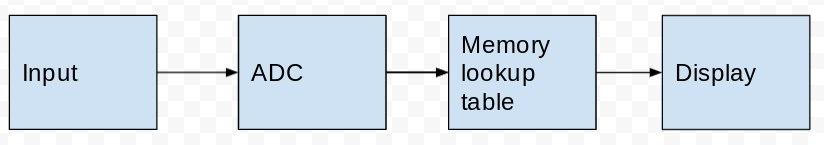
\includegraphics[width=10cm]{images/simpleBlockDiagram.png}
    \caption{The overall simple block diagram of my voltmeter}
    \label{fig:simpleBlockDiagram}
\end{figure}
\noindent I then worked out what components I would need to use for each subsystem and how they would be connected together.
\begin{figure} [H]
    \centering
    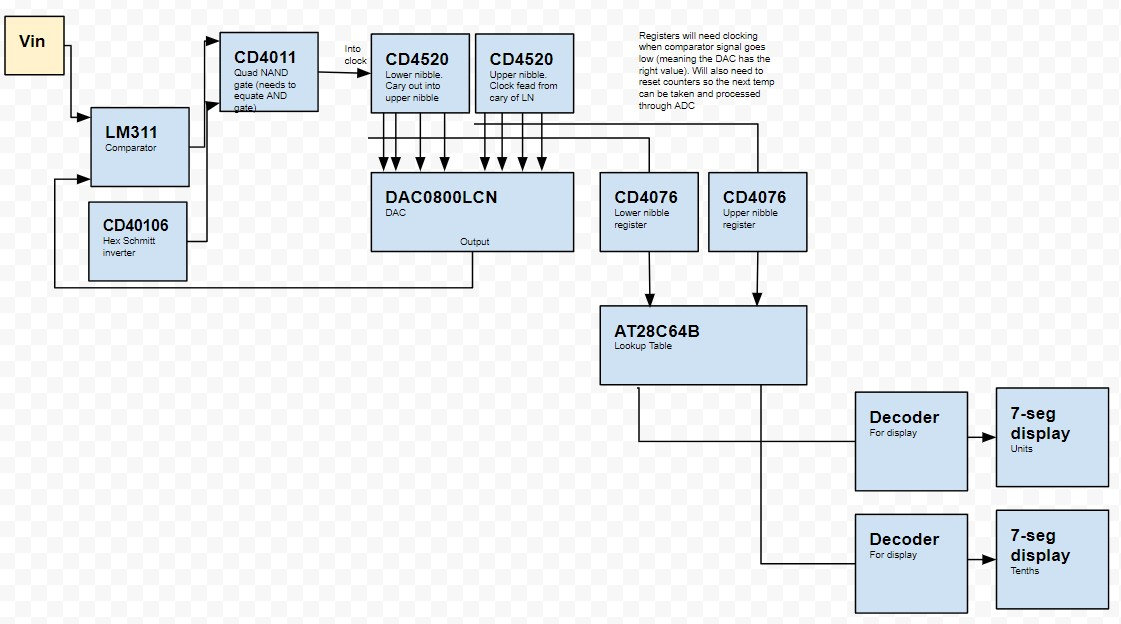
\includegraphics[width=0.9\textwidth]{images/blockDiagram3Updated.jpg}
    \caption{Diagram showing how chips interact}
    \label{fig:blockDiagramSubsystems}
\end{figure}
\noindent\textit{NB: Some wires have been omitted from the diagram above for clarity.}\\
\noindent Also at this stage, I decided on the colours of wires that I would be using. These can be found in the appendix.


%---------------------------CLOCK----------------
\section{Clock Subsystem}
The clock is a fundamental component of the voltmeter as it is used to trigger the counter within the ADC to count, ramping the voltage. This means that the frequency of the clock has to be very fast, around 1KHz; however if it isn't this fast, the clock will still be within acceptable parameters ($\pm400\mathrm{Hz}$). I decided that I would use a Schmitt Inverter Astable.
\subsubsection{Design}
\begin{figure} [H]
    \centering
    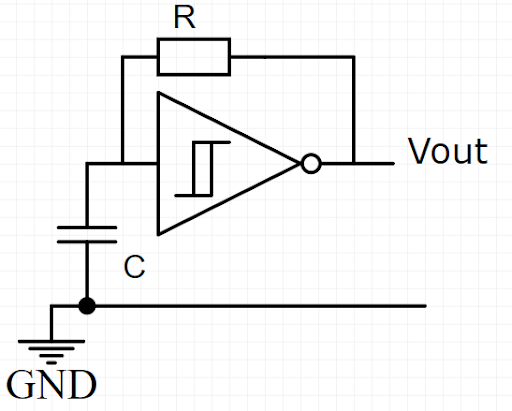
\includegraphics[width=7.5cm]{images/clockCircuitDiagram.png}
    \caption{Circuit diagram of clock subsystem}
    \label{fig:clockCircuitDiagram}
\end{figure}
I then calculated the required component values using the equation  $\displaystyle f = \frac{1}{RC} $ \newline
I knew we had capacitors with capacitance $1\mu F$, so I substituted that along with my desired frequency of 1KHz into the equation then rearranged to calculate the value of the resistor.
\vspace{3mm} \newline
$\displaystyle 1\times10^{3} = \frac{1}{R\times(1\times10^{-6})}$\vspace{3mm} \newline
$\displaystyle R = \frac{1}{{1\times10^{3}}\times(1\times10^{-6})}$\vspace{3mm} \newline
$R = 1000$\vspace{1mm} \newline
\noindent The resultant component values are: \newline
\indent $C=1\mu F$\newline
\indent $R=1K\Omega$
\subsubsection{Building \& Testing}
The clock subsystem was the first subsystem that I constructed.
I tested this by connecting the output of the clock to the oscilloscope probe and using its digital readout to tell me the frequency.
During testing, I found out that the clock’s frequency isn’t 1KHz, however it is 1.36KHz which is acceptable as it is less than 1.4KHz which is the upper parameter. This is because as long as the clock is relatively fast the functionality of my voltmeter won’t be damaged.

\begin{figure} [H]
    \centering
    \begin{minipage}[t]{0.45\textwidth}
        \centering
        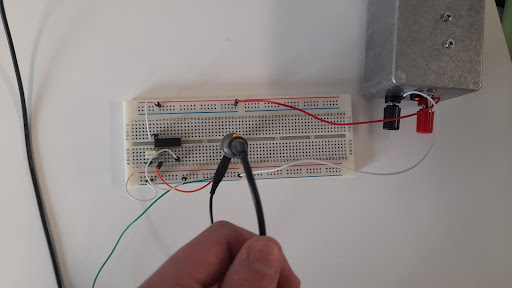
\includegraphics[width=0.9\textwidth]{images/clockTesting1.jpg}
        \caption{Top-down shot of the clock on a breadboard connected to the power supply with an oscilloscope test probe connected to the output of the clock}
        \label{fig:clockTesting1}
    \end{minipage}\hfill
    \begin{minipage}[t]{0.45\textwidth}
        \centering
        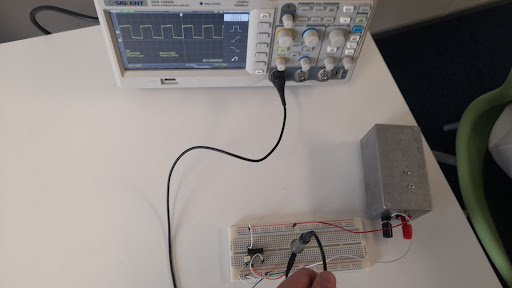
\includegraphics[width=0.9\textwidth]{images/clockTesting2.jpg}
        \caption{View of the oscilloscope and breadboard}
         \label{fig:clockTesting2}
    \end{minipage}
\end{figure}
\begin{figure}[H]
    \centering
    \begin{minipage}[t]{0.45\textwidth}
        \centering
        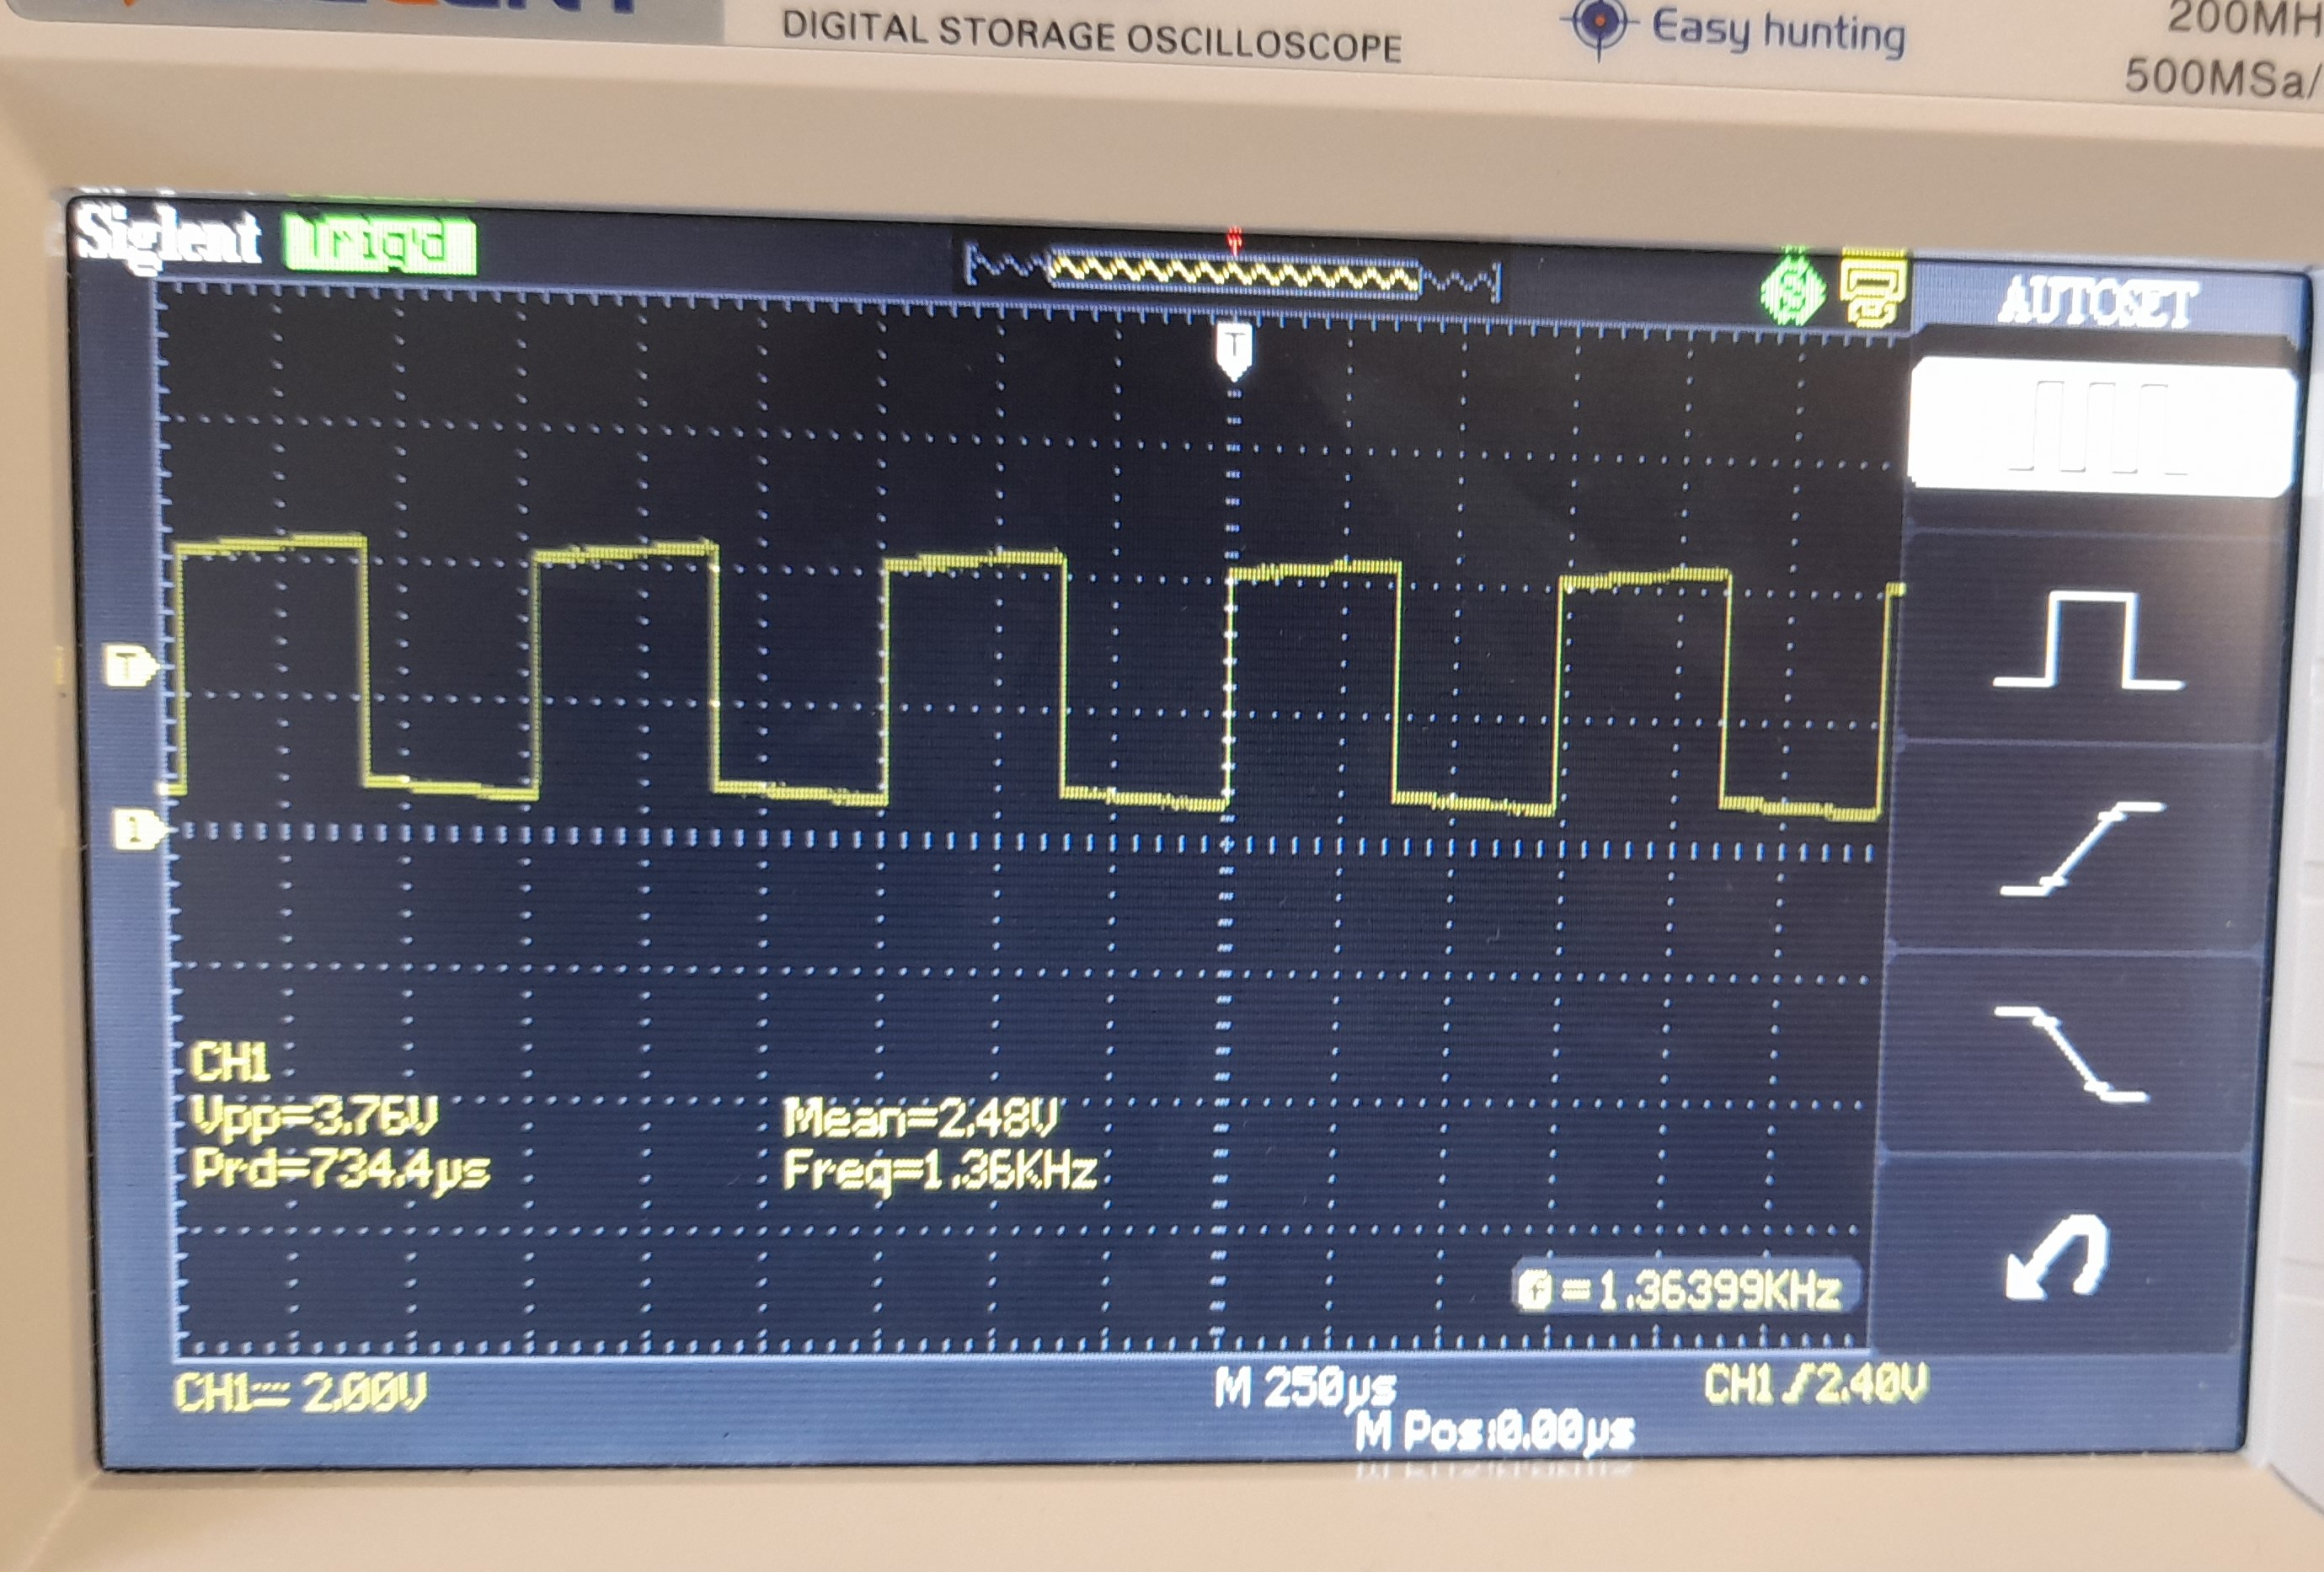
\includegraphics[width=0.9\textwidth]{images/clockOscZoomed.jpg}
        \caption{Output of clock shown on an oscilloscope}
        \label{fig:clockOsc}
    \end{minipage}\hfill
    \begin{minipage}[t]{0.45\textwidth}
        \centering
        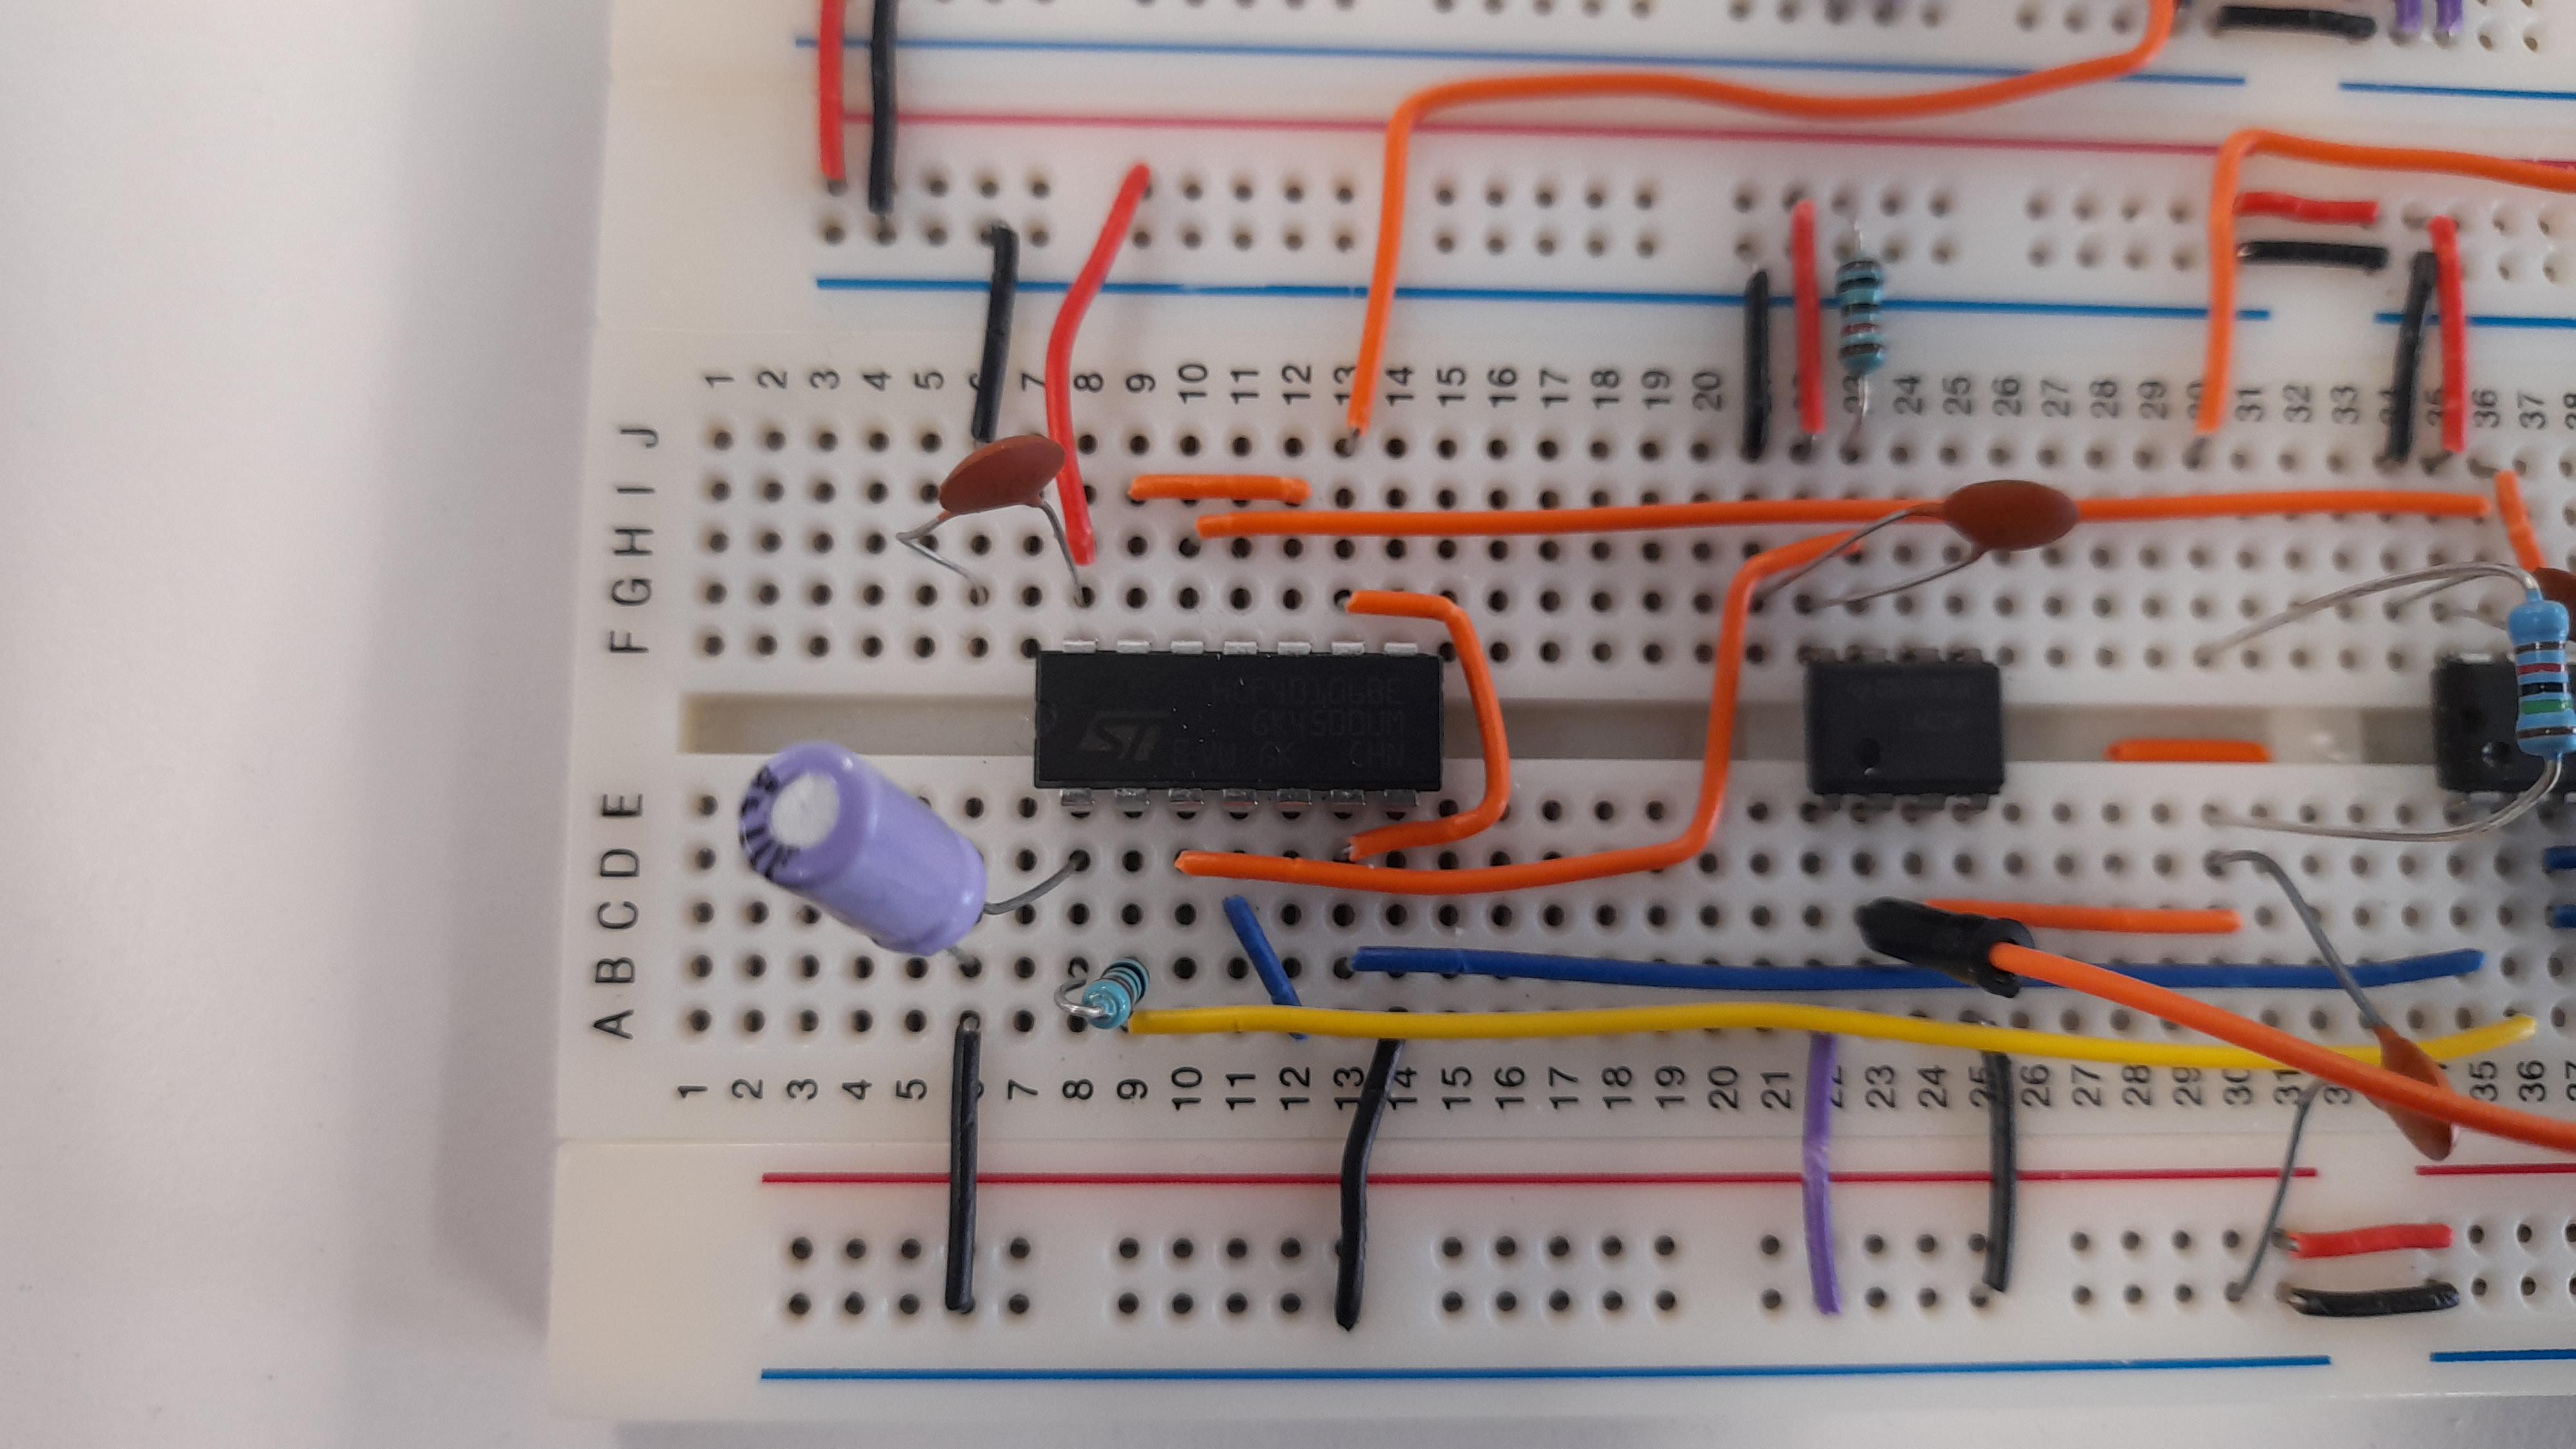
\includegraphics[width=0.9\textwidth]{images/clockNeatened.jpg}
        \caption{Neatened clock subsystem}
         \label{fig:clockNeatWires}
    \end{minipage}
\end{figure}

\noindent After building this, I evaluated some of the different subsystems I could have used instead of the Schmitt astable. I could have used a 555 timer astable, however this would have resulted in me having an extra chip on my breadboards, as I would still need to use Schmitt inverters in a delay line later in the building process. Alternatively, I could have used a Crystal Oscillators. The additional accuracy which this provides would not be necessary. \newline
This subsystem is within the acceptable parameters I set in my design and I am happy with it.

\section{Ramp Analogue to Digital Converter(ADC)}
I decided to use a ramp ADC because my output wouldn’t need an extremely high sample rate and it uses fewer components than the flash ADC. If I was to use a flash ADC in my project where I need 8-bit outputs, I would need 256 comparators \& 256 resistors as well as a priority encoder large enough to handle 256 inputs. Using a ramp ADC means I only need 6 ICs as well as a handful of other components. \newline
The ramp analogue to digital converter is a very complex system with lots of different components and subsystems within it. For this reason, within my report, it will be broken down into the following subsystems (this is also the order in which I constructed them):
\begin{itemize}
    \item Digital to Analogue converter;
    \item Counter;
    \item Comparator;
    \item Delay Line;
    \item Latch;
    \item Low Pass Filter.
\end{itemize}
\subsection{Digital to Analogue Converter}
\subsubsection{Design}
As part of my research, I found out that digital to analogue converters come in DIP packages and opted to use a DAC0800LCN. This DAC requires a +5V, 0V and -5V supply. \newline
I used the datasheet (https://www.ti.com/lit/ds/symlink/dac0800.pdf) of the DAC0800LCN to work out how it is connected.
\begin{figure} [H]
    \centering
    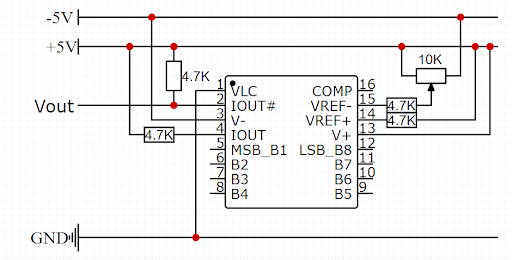
\includegraphics[width=0.6\textwidth]{images/dacCircuitDiagram.png}
    \caption{Circuit diagram of the DAC}
    \label{fig:dacCircuitDiagram}
\end{figure}
\noindent \textit{NB: The inputs (B1 through B8) will be connected as shown in the counter circuit diagram}

\subsubsection{Building \& Testing}
I connected the DAC on its own first to ensure that it worked as expected before I combined it with the rest of the ADC. To test it, I fed a binary sequence into it (using the +5V rail and 0V rail to provide logic 1 and 0 respectively) and measured the output of the DAC using the voltmeter function of a multimeter. \newline
The output of the DAC was extremely noisy. At the time of building the DAC, I disregarded this and assumed that it would be fine. However, as I constructed more of the ADC, I realised that the noisy output was causing lots of problems. Initially to rectify this, I tried adding decoupling capacitors to the +5V input of all chips on my breadboards. This should have reduced the noise from the power rails. This was unsuccessful, so I then added a low lass filter to the output of the DAC (this goes into the inverting input of the comparator). This is because the output of the DAC was at a frequency of 4MHz. As this was so high, I was able to select a break frequency which would filter the noise out and leave the ramp unaffected. I set the break frequency of the LPF to 10KHz and this solved my problems. The filtered output from the DAC was now clean, meaning it was no longer interfering with the Comparator. See \hyperref[sec:LPF]{Low Pass Filter} section for the circuit diagram as well as the notes from testing the filter.

\begin{figure}[H]
    \centering
    \begin{minipage}[t]{0.45\textwidth}
        \centering
        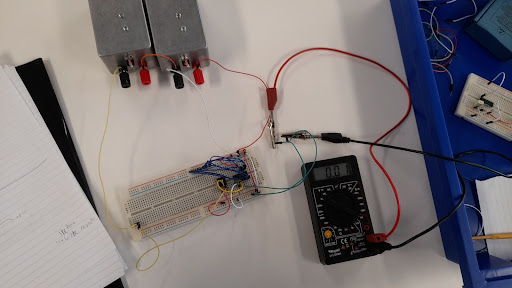
\includegraphics[width=0.9\textwidth]{images/dacTesting1.jpg}
        \caption{The DAC connected to 00000000, giving Vout of 0.01V}
        \label{fig:dacTesting1}
    \end{minipage}\hfill
    \begin{minipage}[t]{0.45\textwidth}
        \centering
        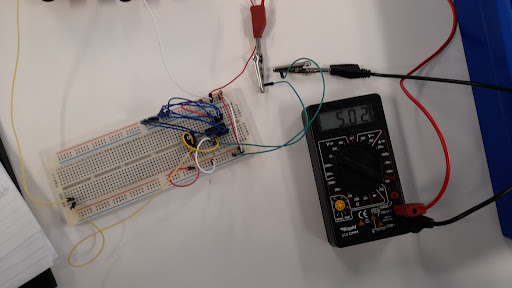
\includegraphics[width=0.9\textwidth]{images/dacTesting2.jpg}
        \caption{The DAC connected to 11111111, giving Vout of 5.02V}
        \label{fig:dacTesting2}
    \end{minipage}
\end{figure}
\noindent The input value 00000000 should have given me exactly 0V and the input value 11111111 should have give me exactly 5V. To obtain these values, I adjusted the potentiometer on pin 15 until the values were correct. The potentiometer is used to provide a reference voltage of 0V to the DAC chip.
\begin{figure}[H]
    \centering
        \begin{minipage}[t]{0.45\textwidth}
        \centering
        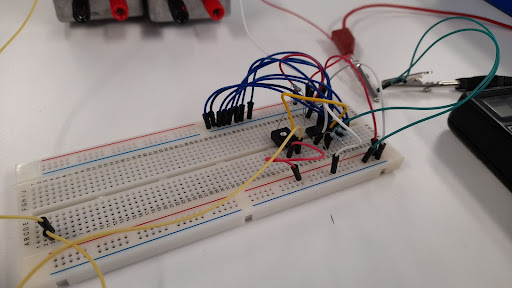
\includegraphics[width=0.9\textwidth]{images/dacTesting3.jpg}
        \caption{The DAC connected with temporary jumper wires on the breadboard}
        \label{fig:dacTesting3}
    \end{minipage} \hfill
    \begin{minipage}[t]{0.45\textwidth}
        \centering
        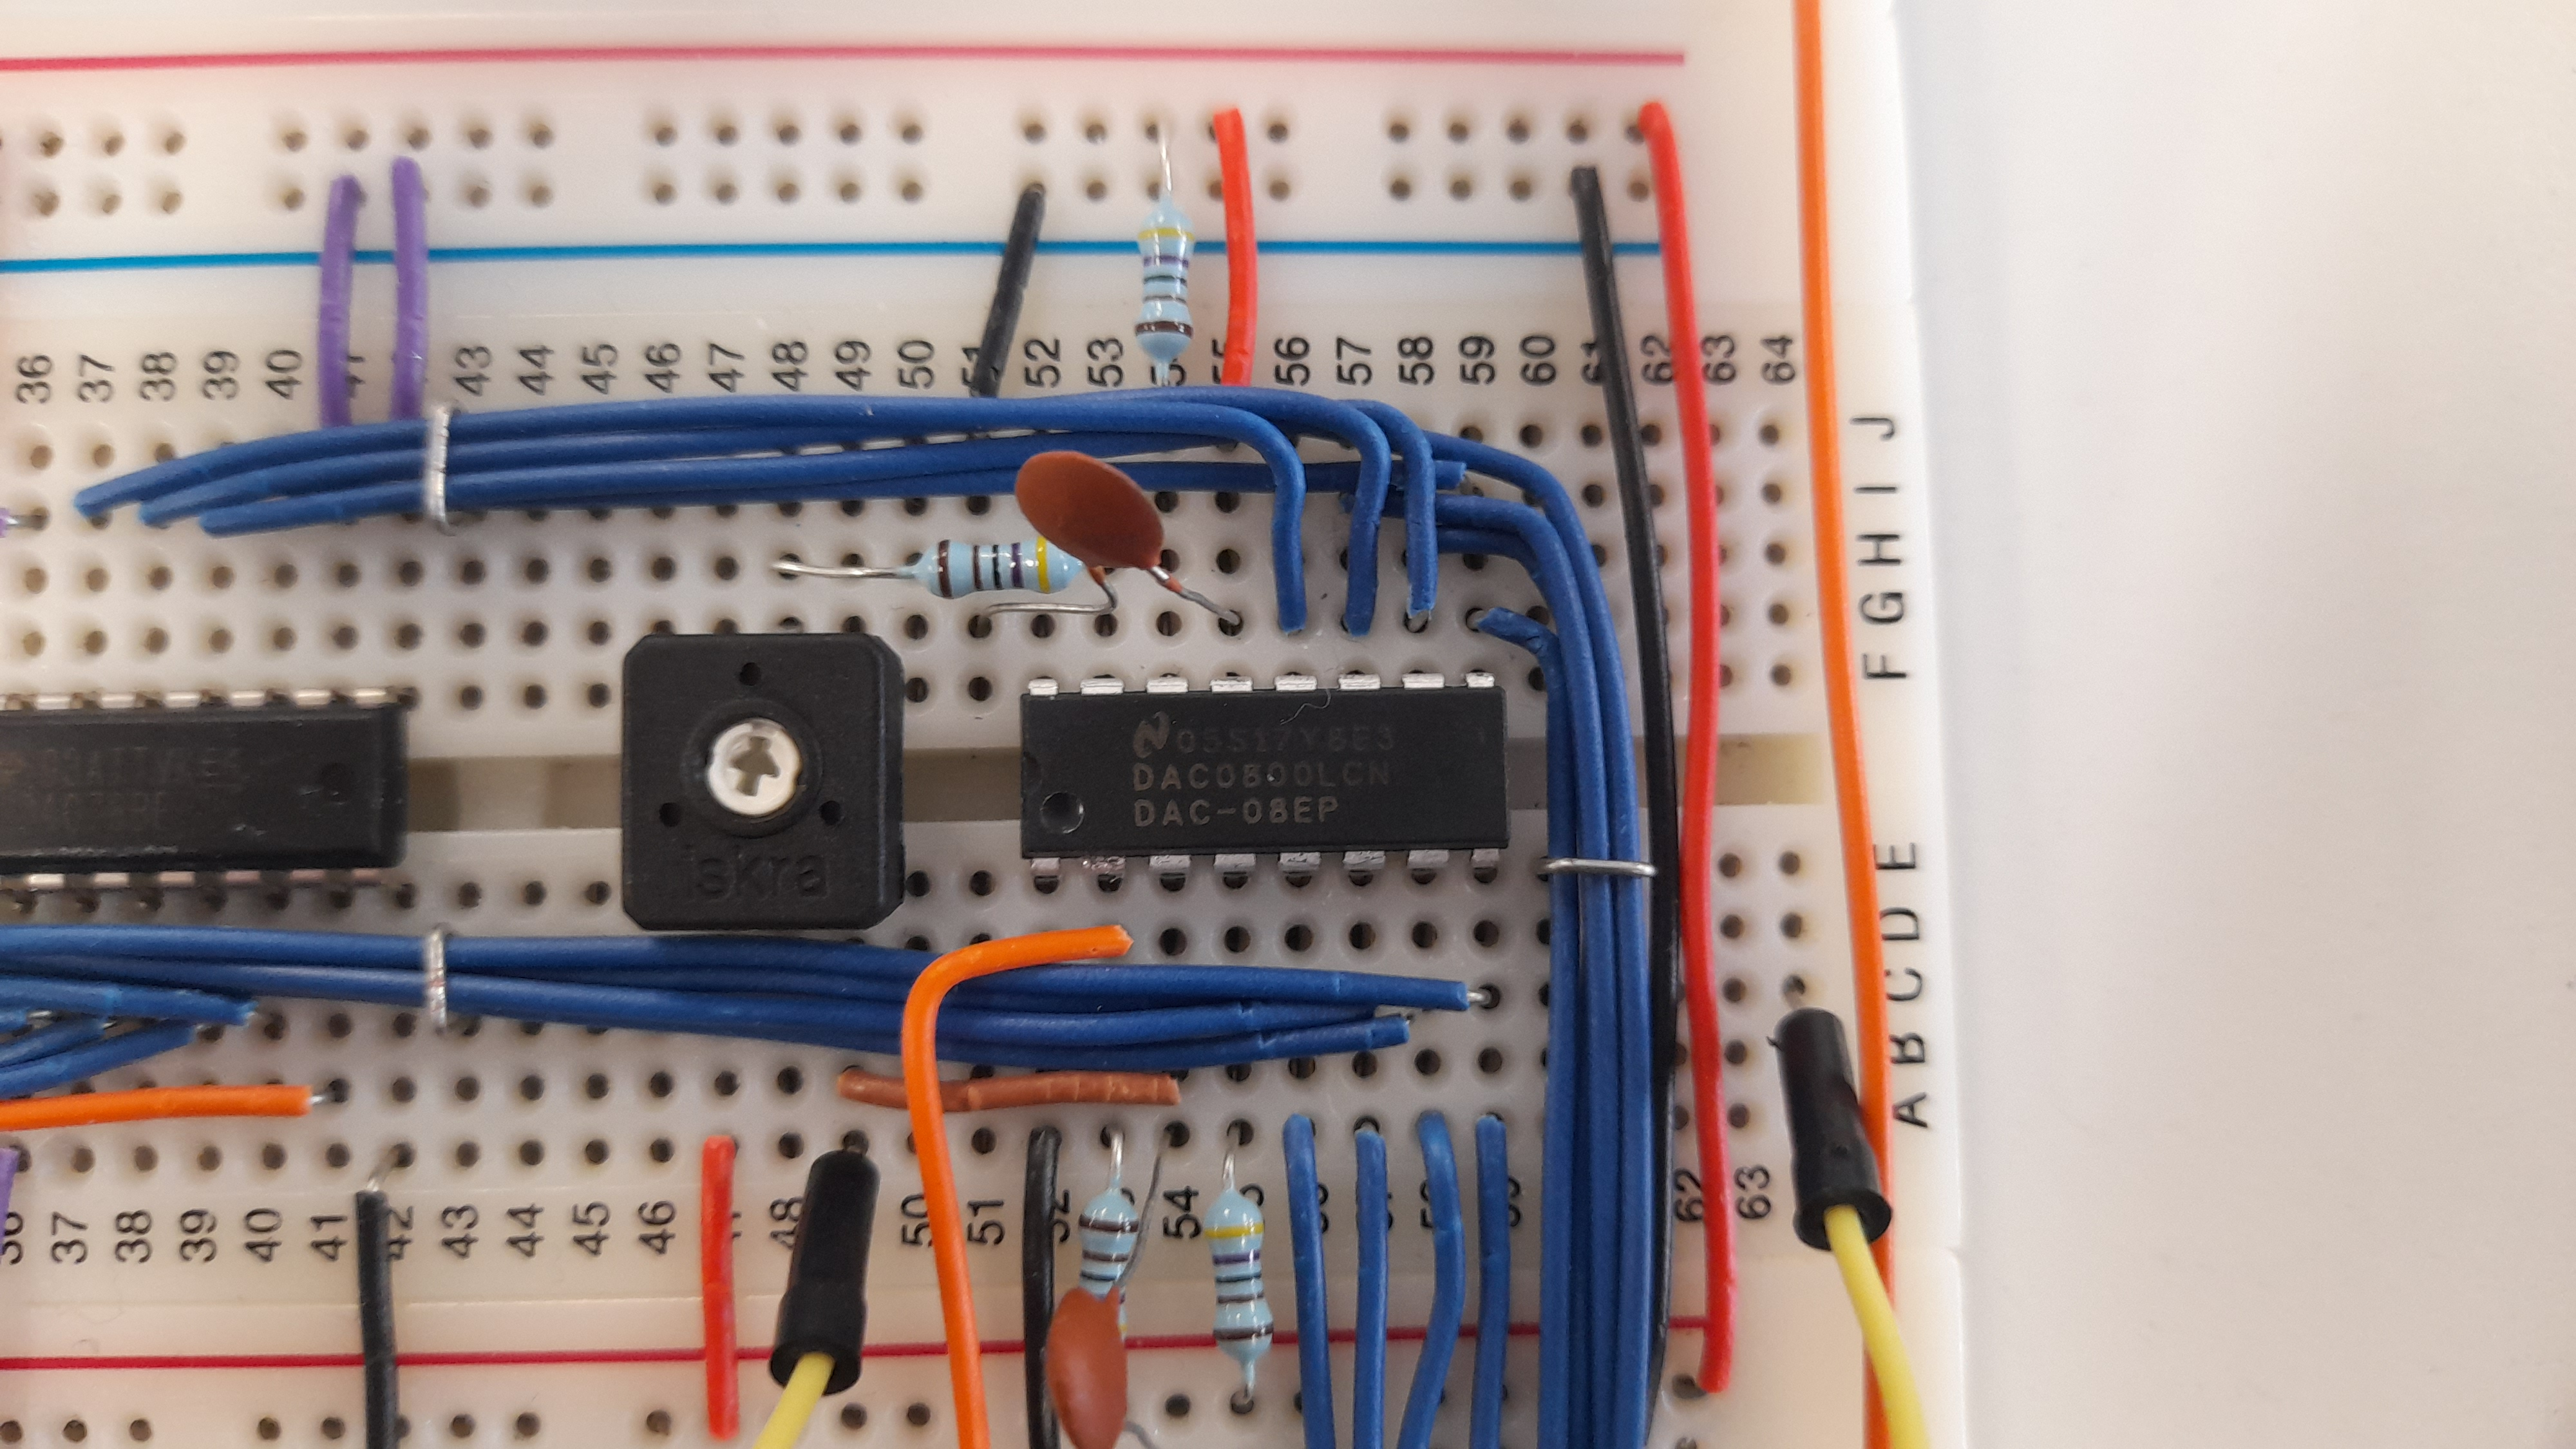
\includegraphics[width=0.9\textwidth]{images/dacNeatened.jpg}
        \caption{Close-up of neatened DAC chip}
        \label{fig:dacNeatenedCloseUp}
    \end{minipage}
\end{figure}
\noindent This subsystem will have to be tested further when I have constructed the counter, as this is what will drive it. \newline
An alternative subsystem I could have used is a resistor ladder DAC or a binary weighted DAC. Overall, the most compact method which I could have used is the fully integrated DAC chip. The binary weighted DAC would have required an additional 12 resistors as well as two more op amps. The resistor ladder DAC would have required more than 16 resistors. 
\subsection{Counter}
The counter will be used to provide the ramping input which goes into the DAC.
\subsubsection{Design}
To begin designing this subsystem, I looked at the datasheet for the CD4520 and understood how to operate the dual counters in cascaded up counter mode. I then designed the circuit diagram.
\begin{figure}[H]
    \centering
    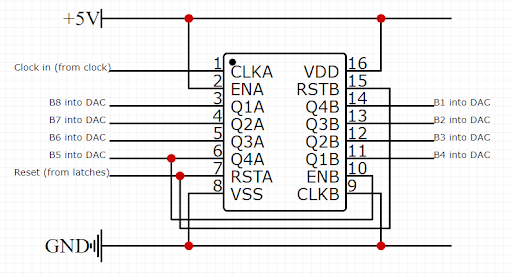
\includegraphics[width=0.6\textwidth]{images/counterCircuitDiagram.png}
    \caption{Circuit diagram of the counter}
    \label{fig:counterCircuitDiagram}
\end{figure}
\subsubsection{Building \& Testing}
I began by connecting the counter together as I specified in my circuit diagram. As I had already built the clock, I connected that to the clock input of counter A, and cascaded into counter B. After constructing the DAC, I was able to test the counters and didn’t get the response I expected.\\ After some troubleshooting, I realised that I hadn’t connected the reset pins to 0V, meaning they were floating, causing the counter to reset randomly, giving me random readings on the output of the DAC. Once I had rectified the mistake, the counter worked as expected.\\
\noindent I then neatened the wires which carried the binary data between the counter and DAC. Before progressing further, I tested this again to ensure it still worked, which it did. The clock wires were still jumper wires as in the final circuit, they wouldn't be connected like this.\\
\noindent I was now able to test the DAC further. By connecting the probe of the oscilloscope to the output of the DAC, I was able to confirm that the counter was correctly outputting a sequentially increasing binary number and that the DAC was correctly converting this to an analogue signal. I could see this by the fact that the output of the DAC was a ramp waveform with amplitude 5V. 
\begin{figure}[H]
    \centering
    \begin{minipage}[t]{0.45\textwidth}
        \centering
        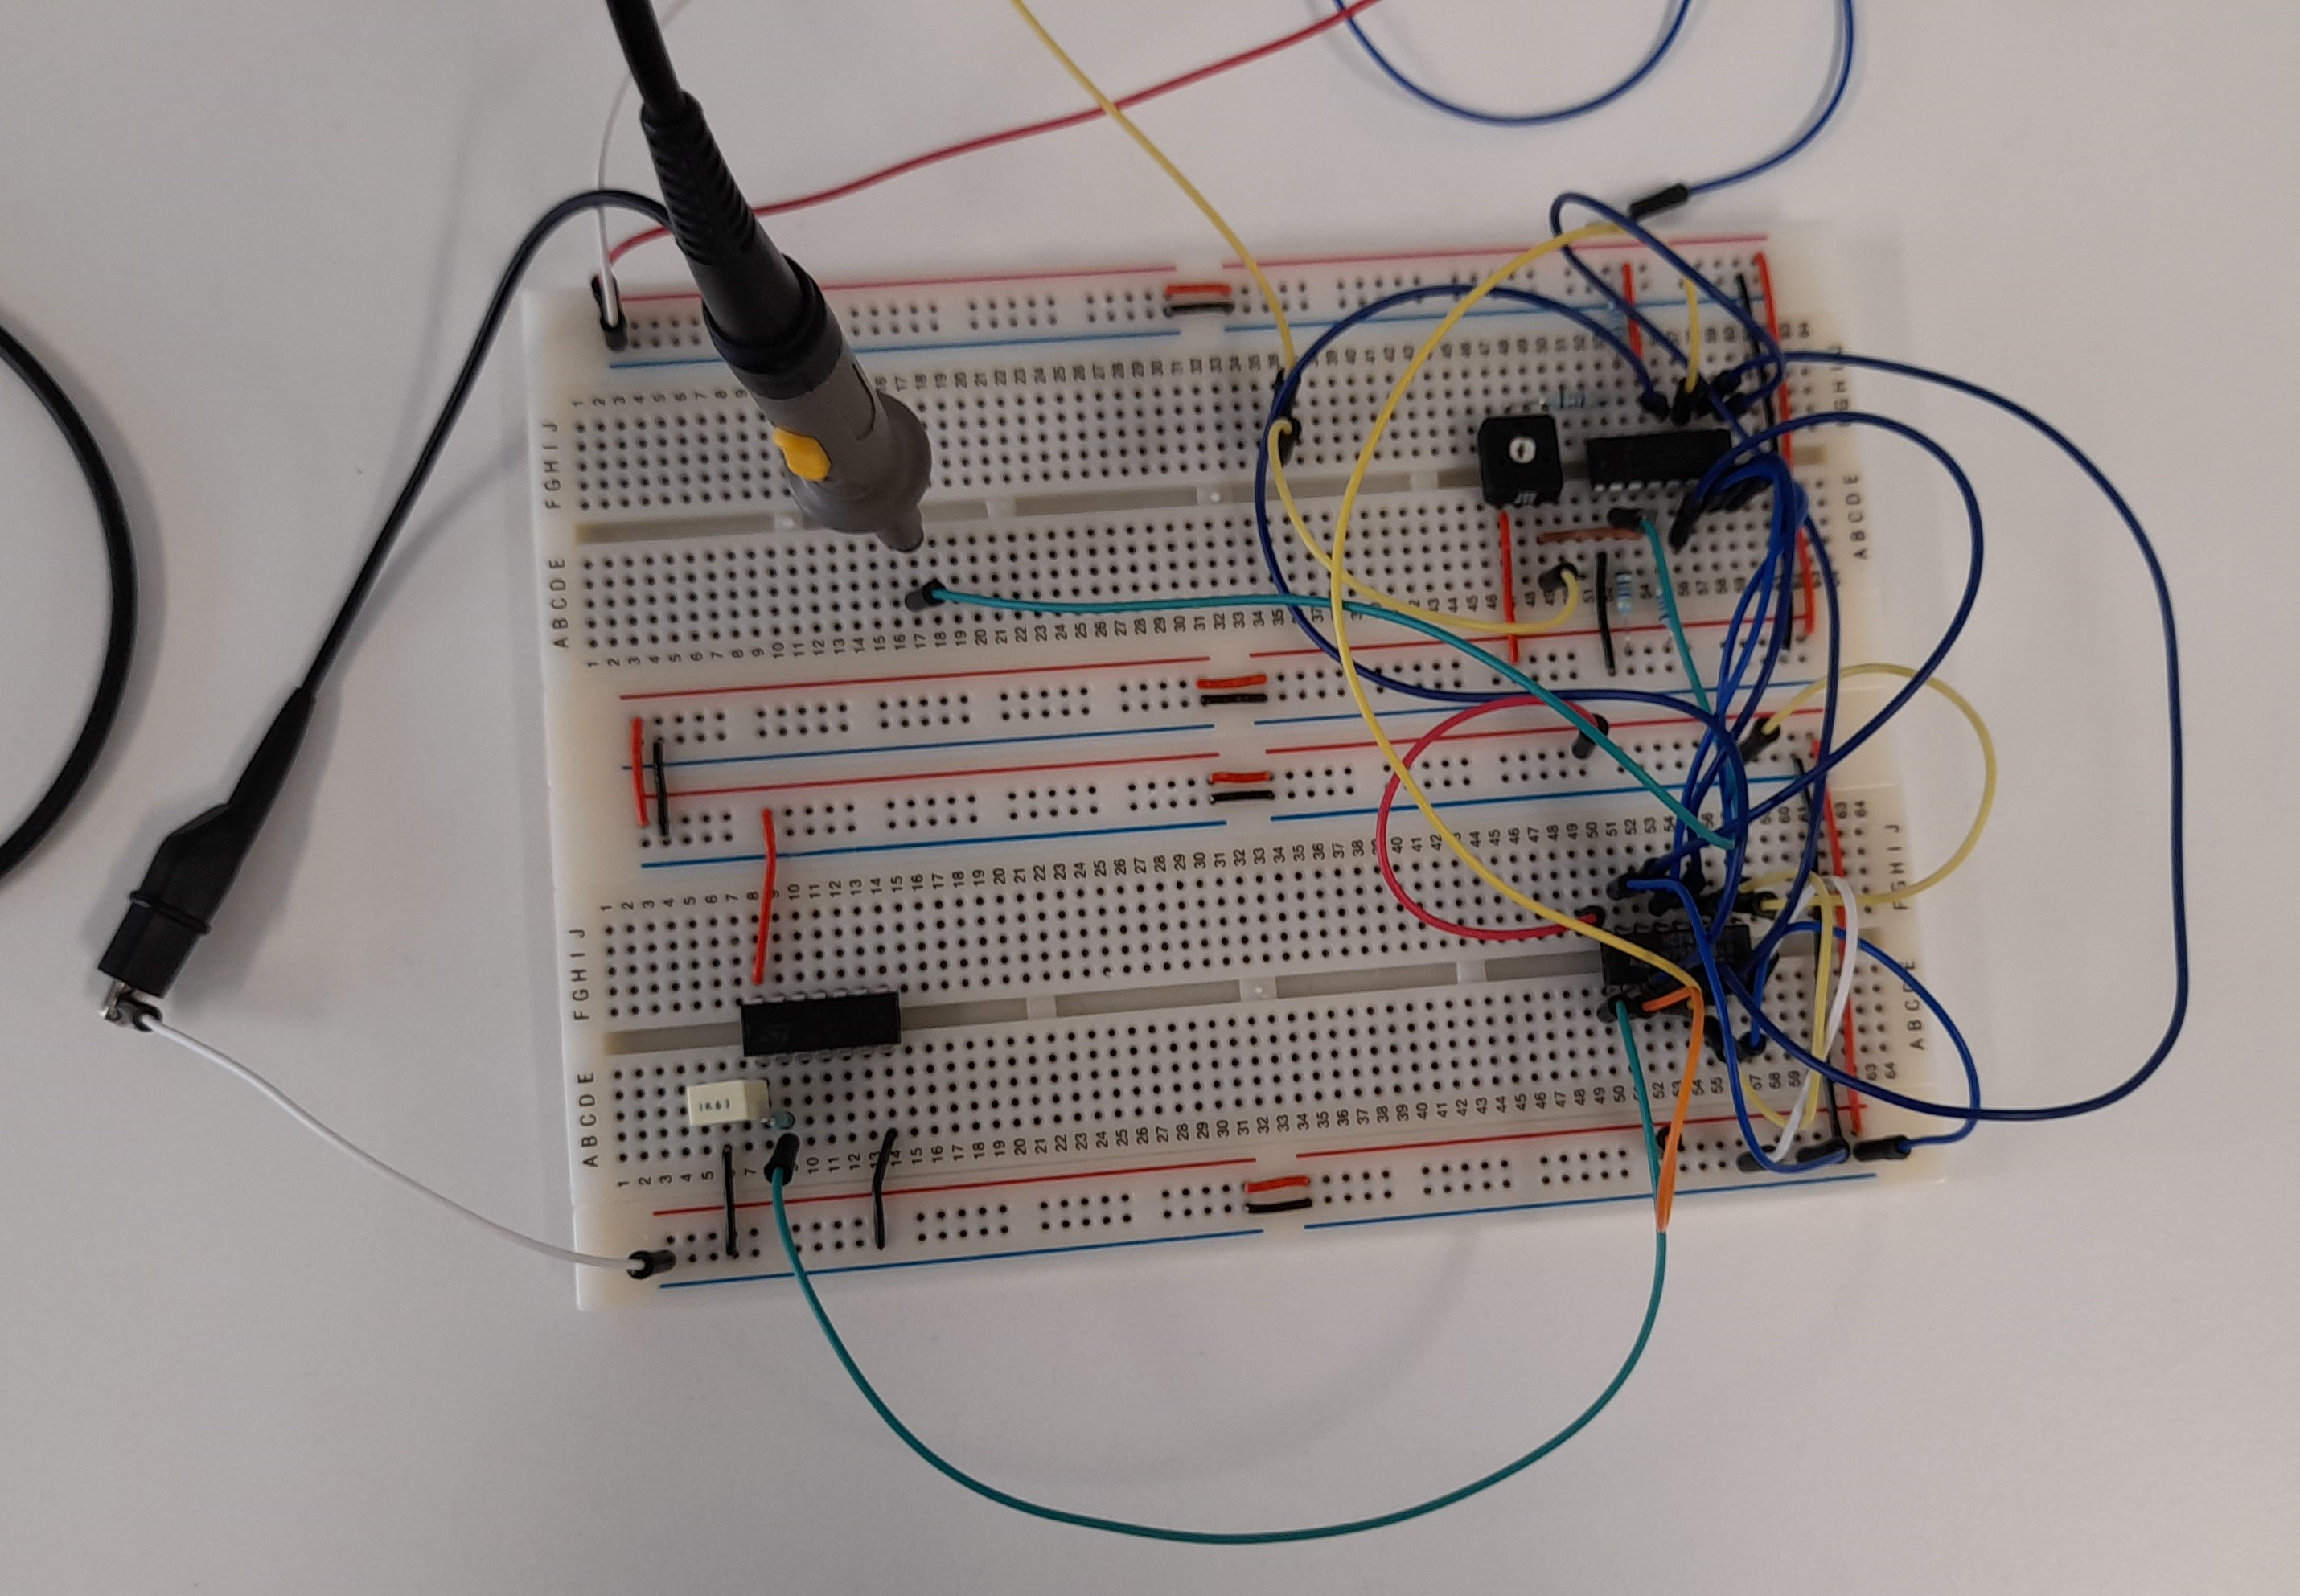
\includegraphics[width=0.9\textwidth]{images/counterJumperTestCropped.jpg}
        \caption{The counter, clock and DAC connected together with temporary jumper wires}
        \label{fig:counterTesting1}
    \end{minipage}\hfill
    \begin{minipage}[t]{0.45\textwidth}
        \centering
        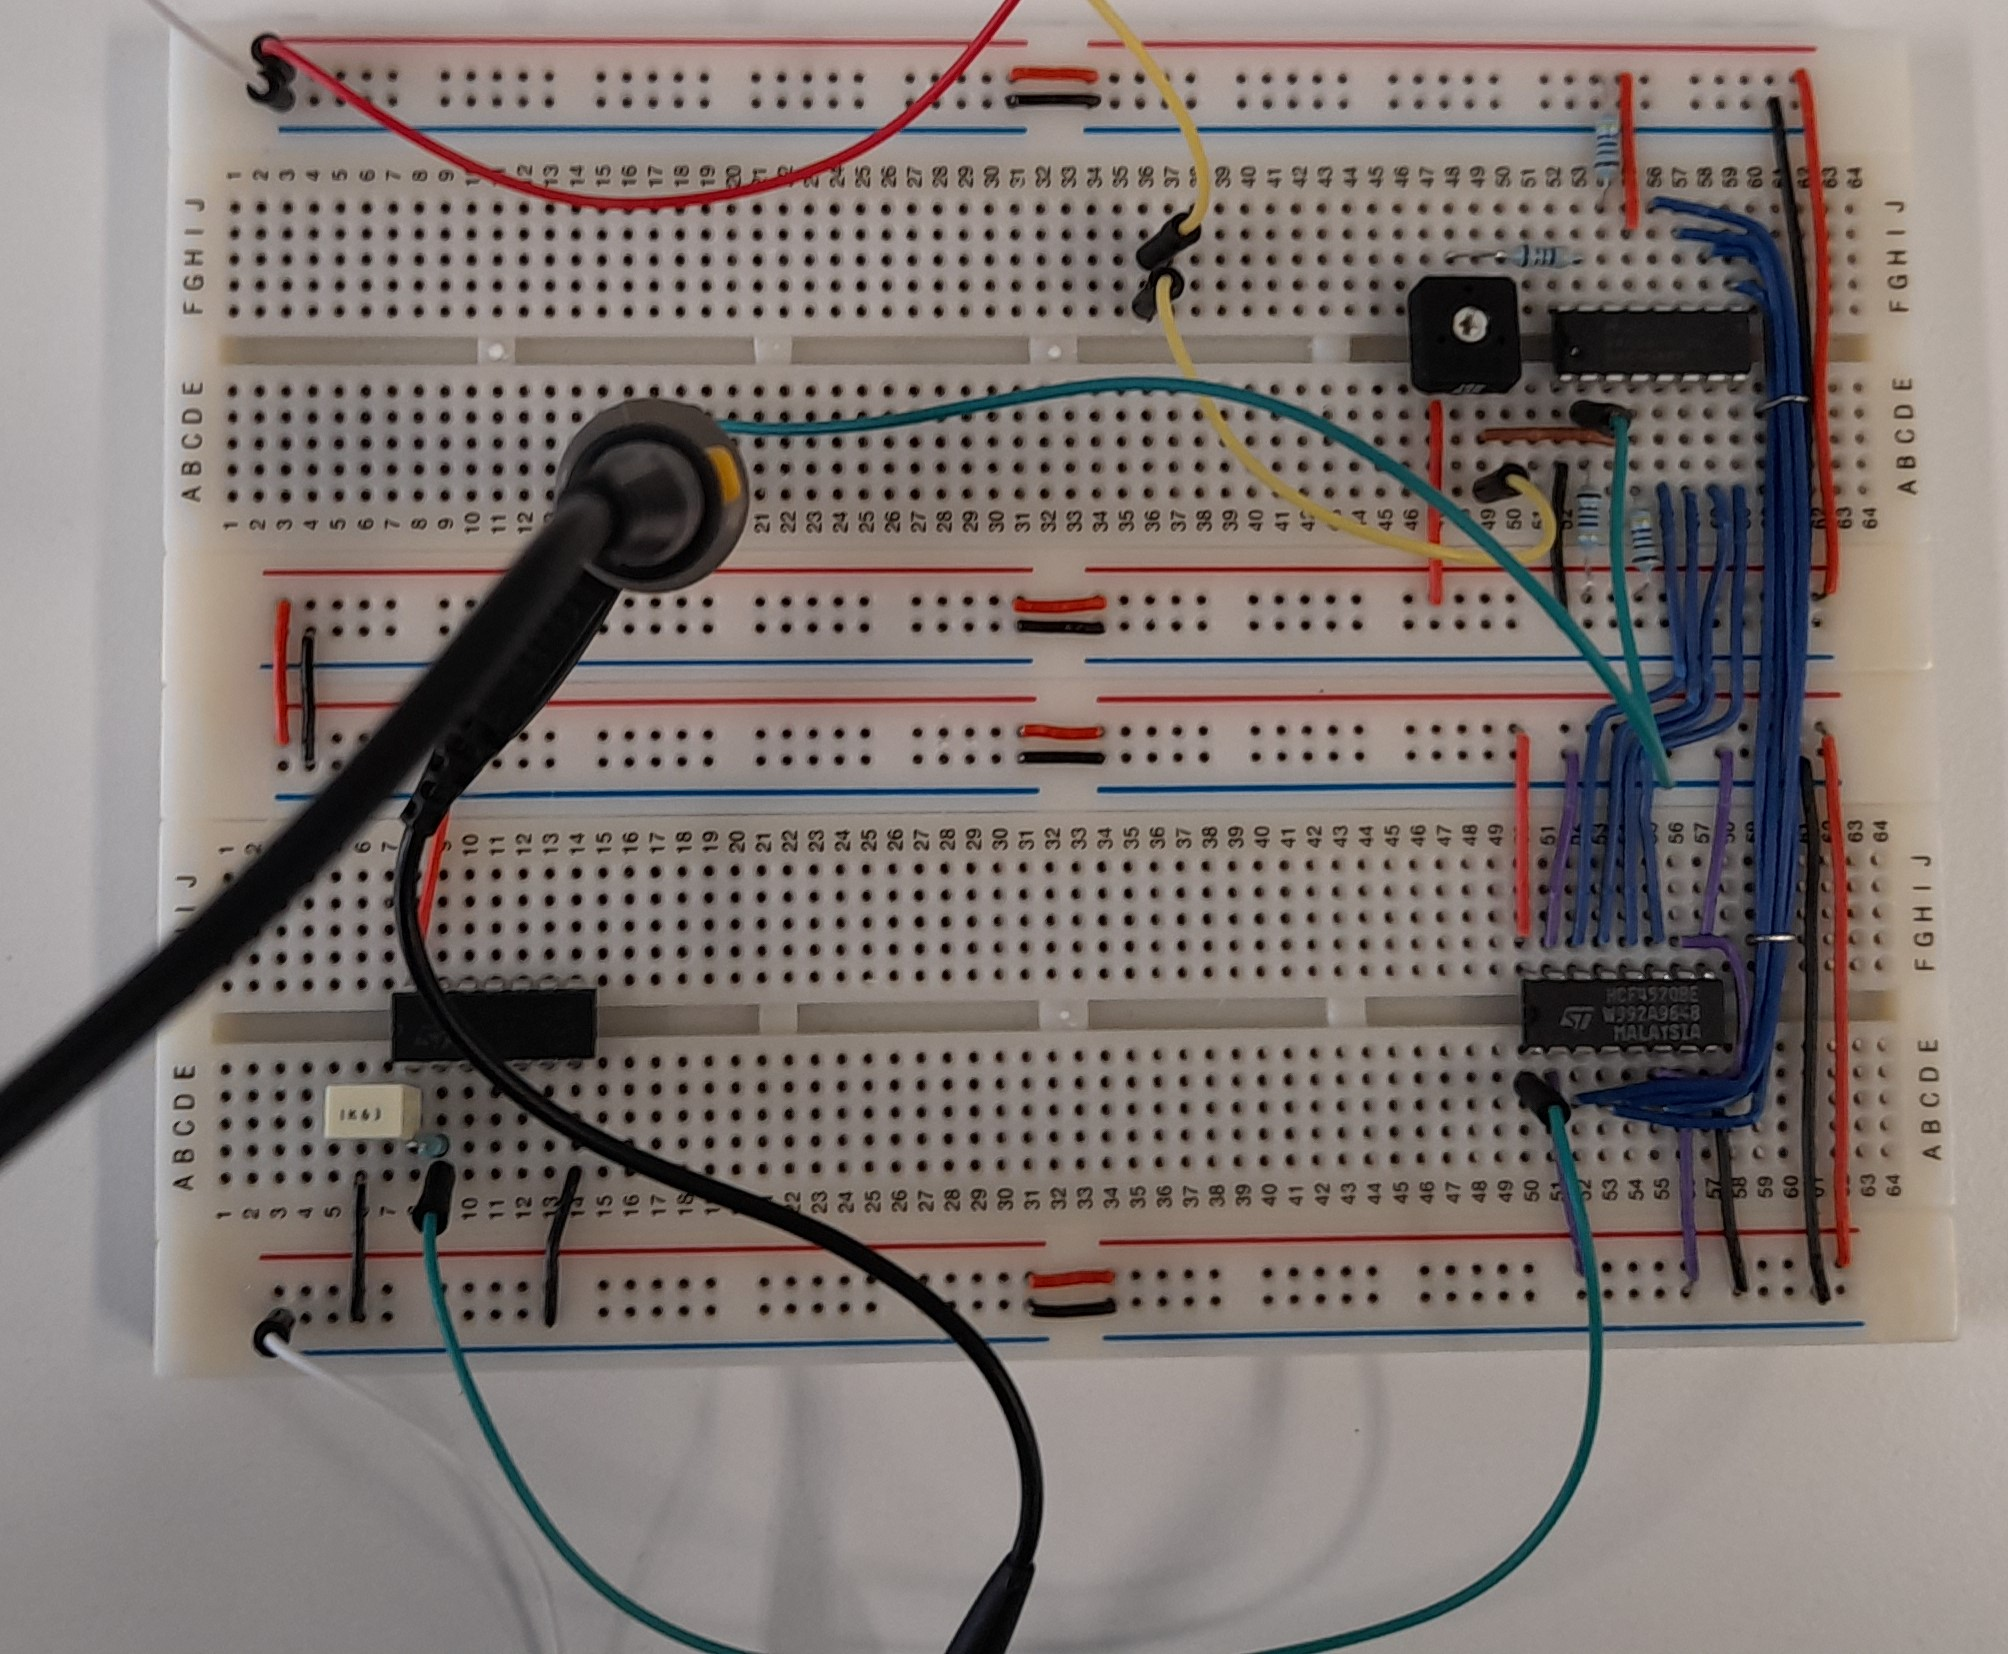
\includegraphics[width=0.9\textwidth]{images/counterNeatenedTestCropped.jpg}
        \caption{Post wire neatening}
        \label{fig:counterTesting2}
    \end{minipage}
\end{figure}
\begin{figure}[H]
    \centering
    \begin{minipage}[t]{0.45\textwidth}
        \centering
        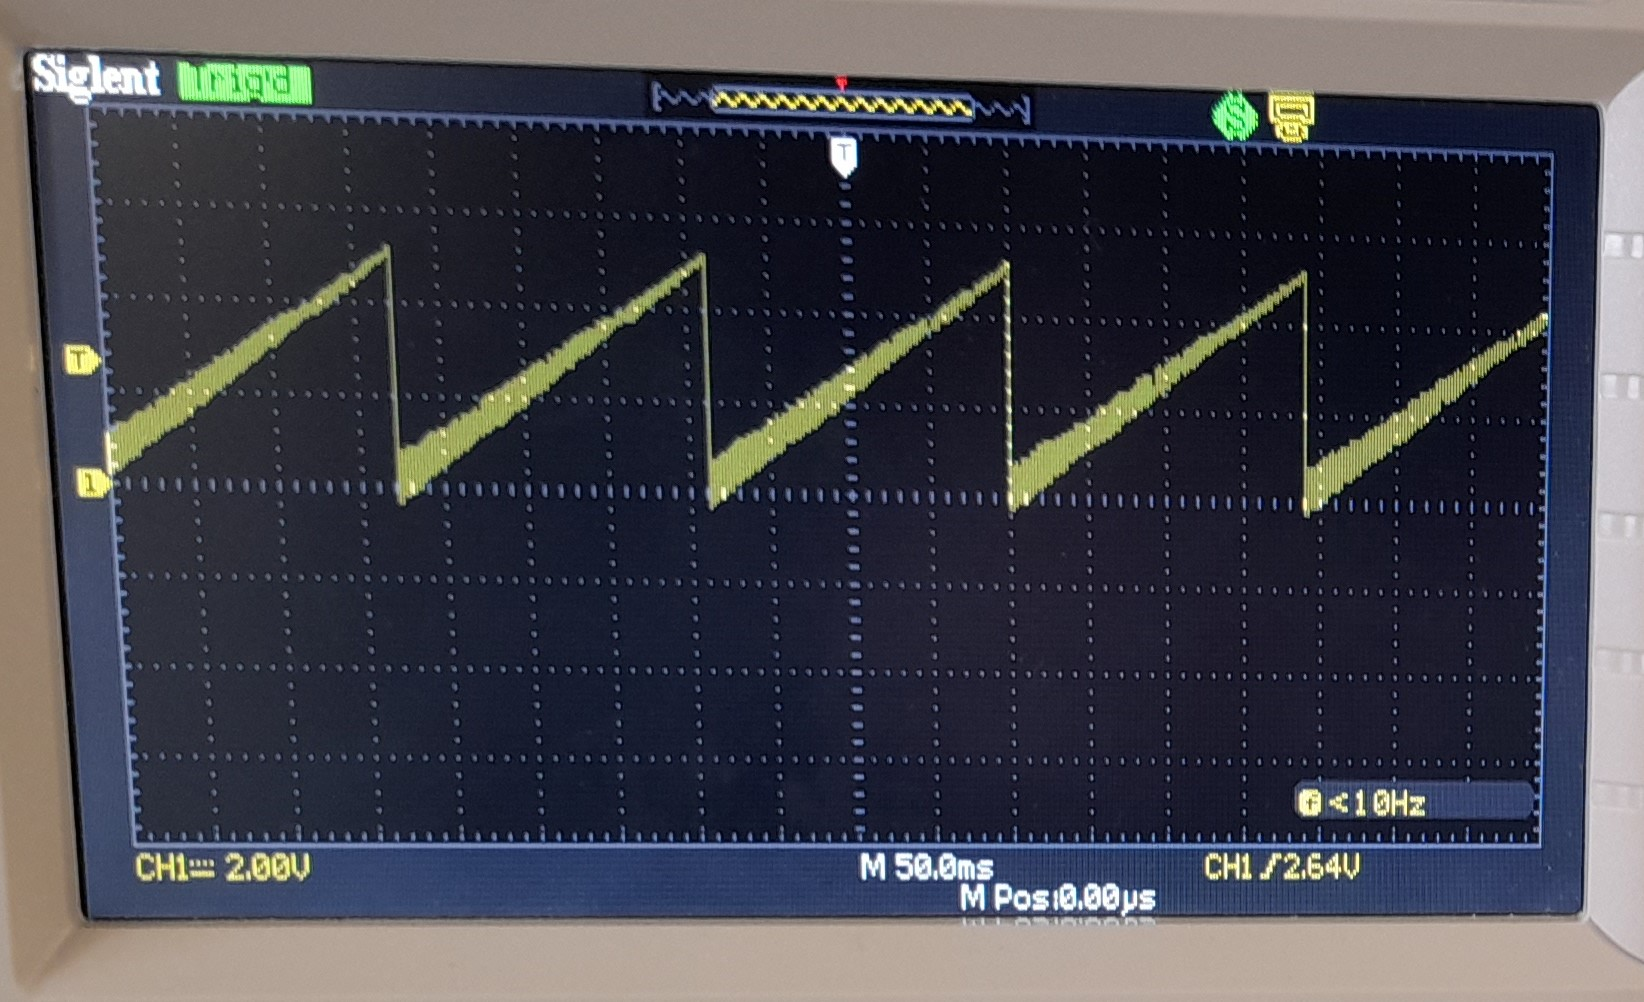
\includegraphics[width=0.9\textwidth]{images/counterOutputZoomed.jpg}
        \caption{Ramp voltage output of the DAC}
        \label{fig:counterOutput}
    \end{minipage}\hfill
    \begin{minipage}[t]{0.45\textwidth}
        \centering
        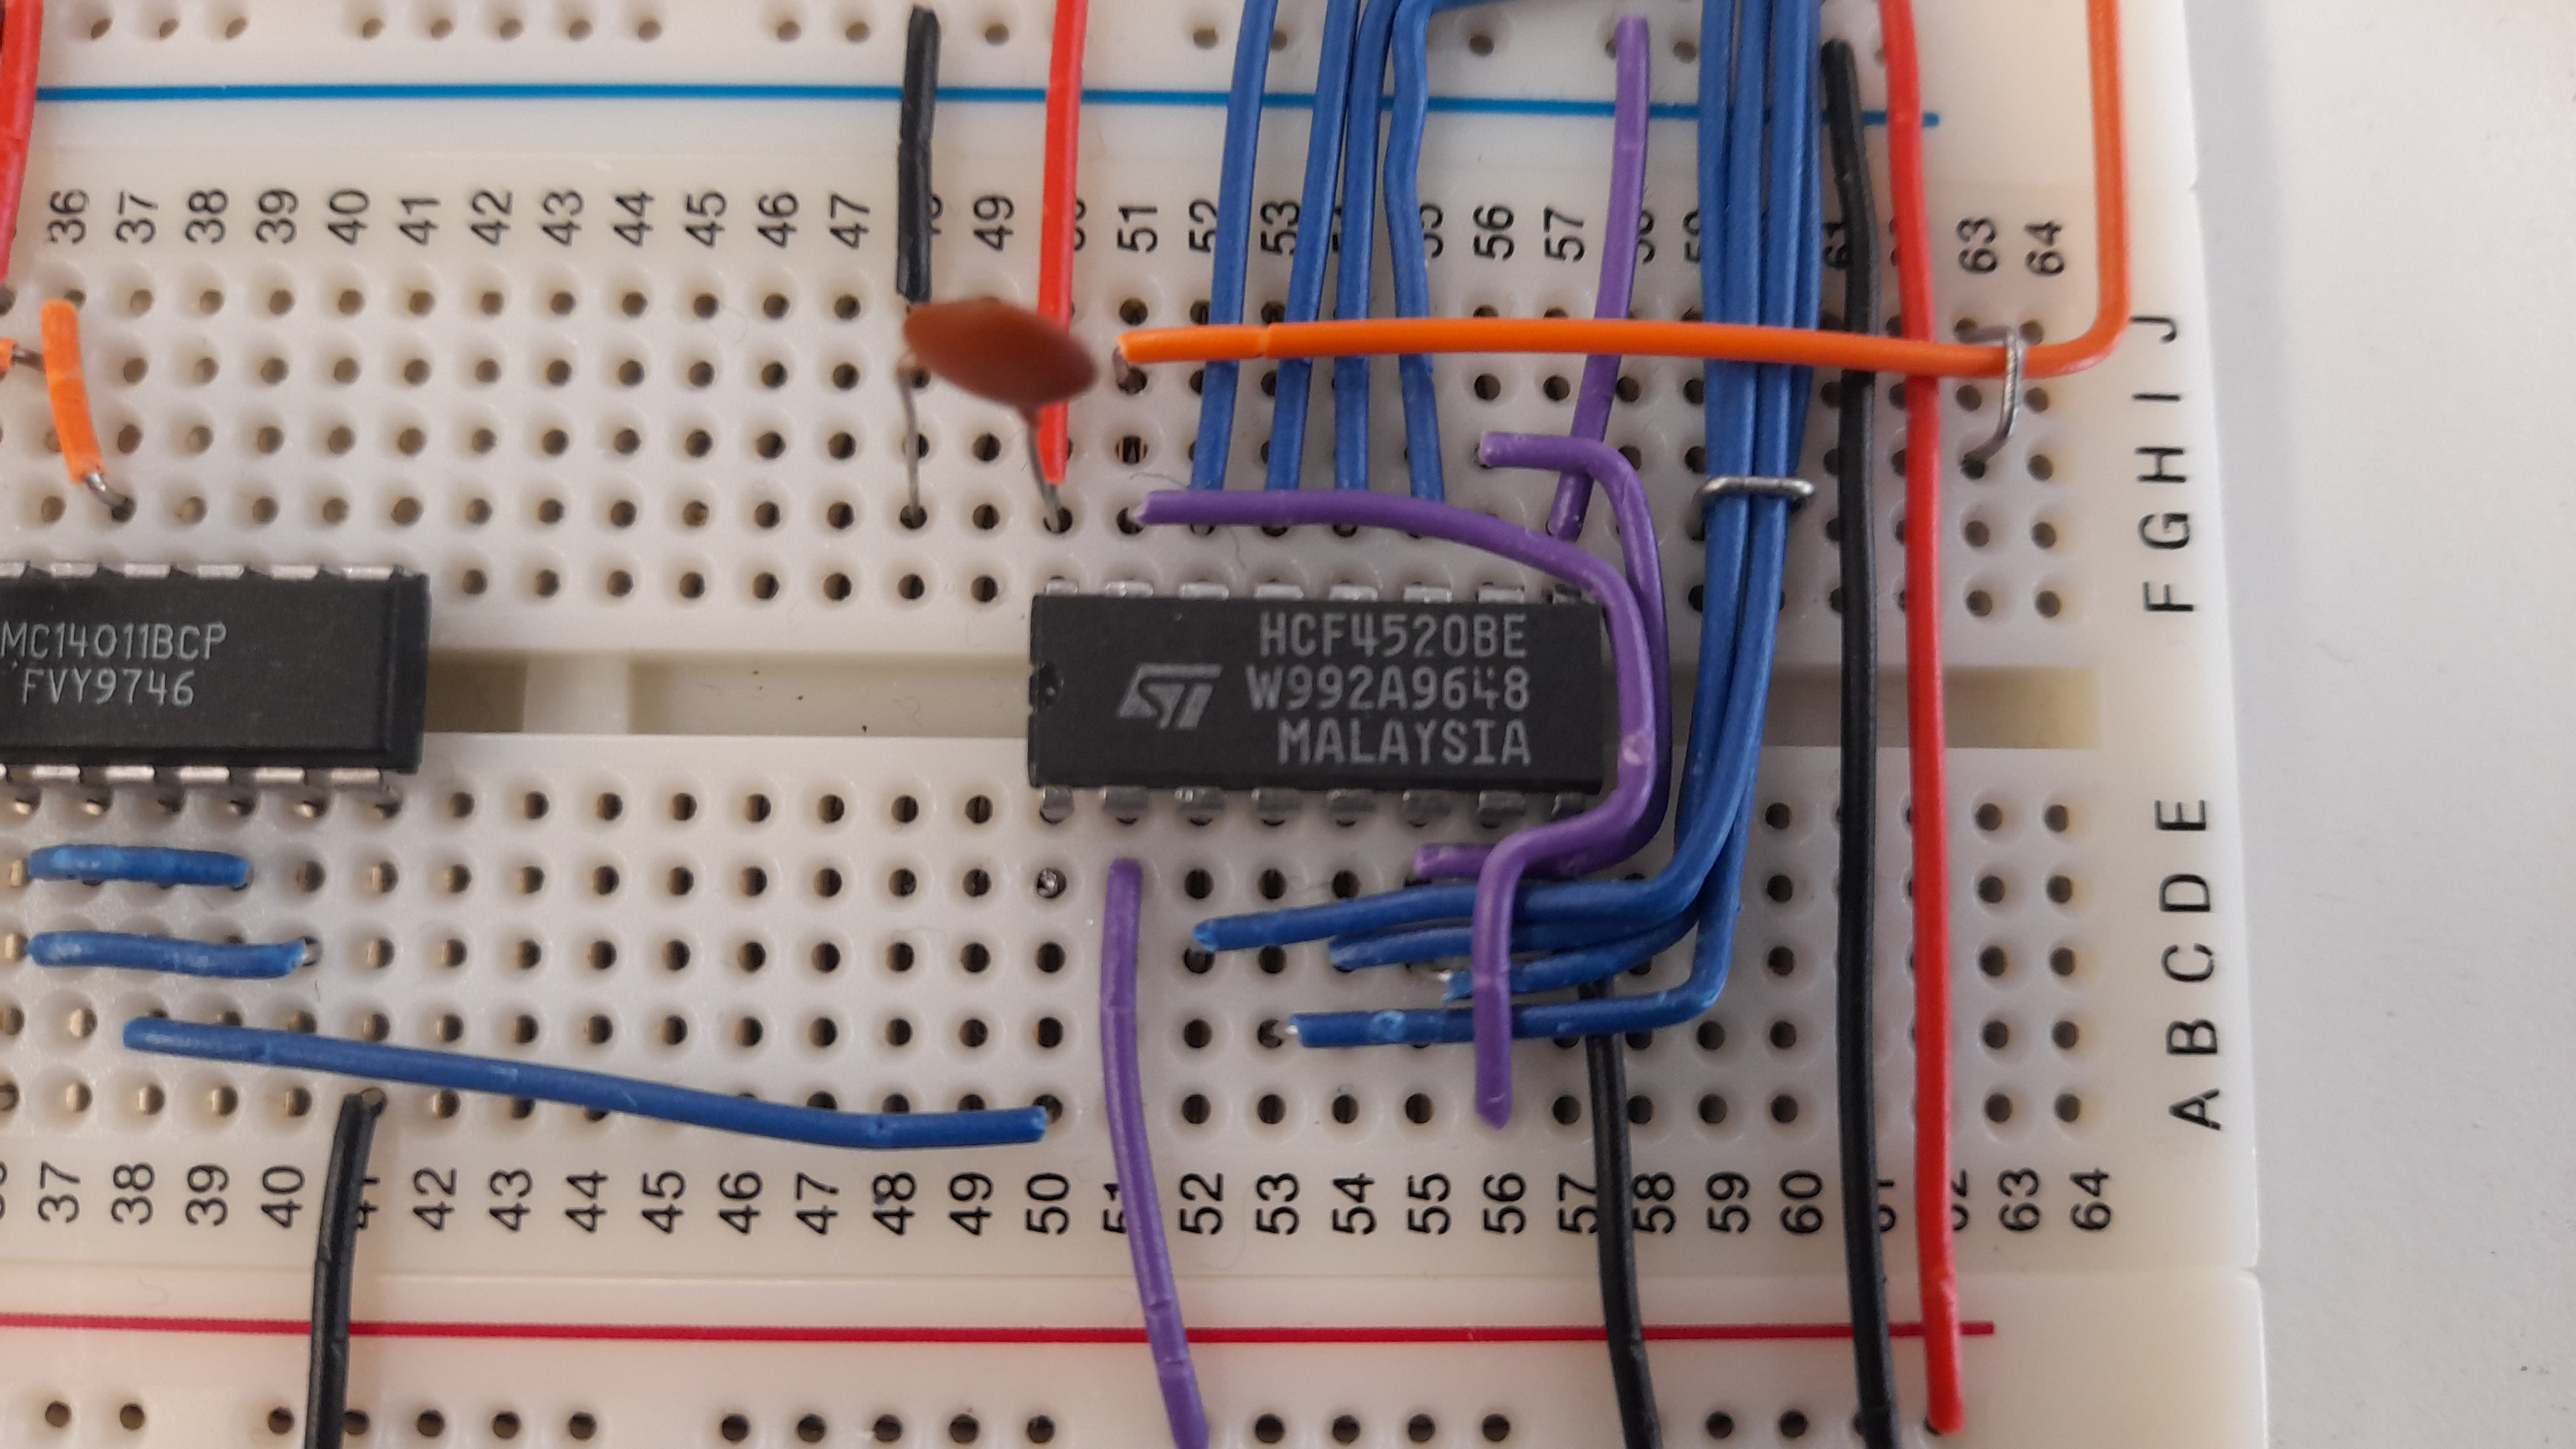
\includegraphics[width=0.9\textwidth]{images/counterNeatenedFinal.jpg}
        \caption{Close-up of neatened counter chip}
        \label{fig:counterCloseUpNeatened}
    \end{minipage}
\end{figure}
\noindent The noisy output from the DAC can be seen in Figure \ref{fig:counterOutput}, especially at the lower part of the ramp. \newline
An alternative subsystem I could have used is to manually construct the counters out of D-Flip-Flops however this would have been an unnecessary level of complexity for no benefit, as well as using lots more components.

\subsection{Comparator}
\subsubsection{Design}
I designed this based on a LM311 comparator and CD4011 IC NAND chip. First I drew out the circuit diagram, using the datasheets of both of the chips.
\begin{figure}[H]
    \centering
    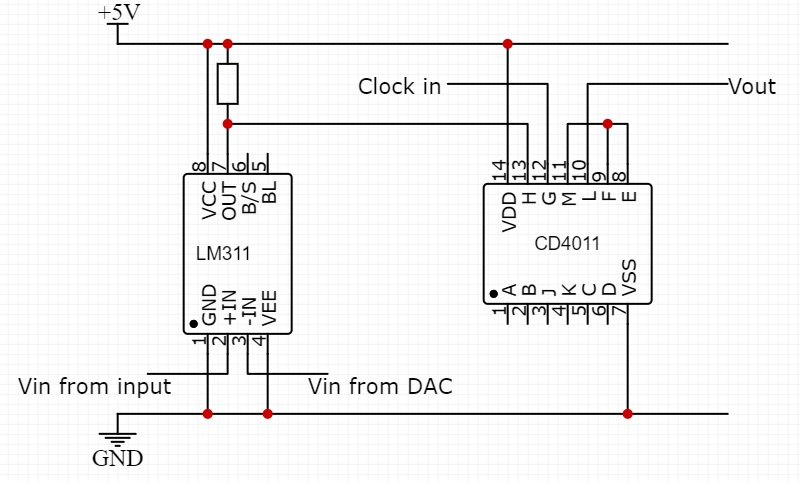
\includegraphics[width=0.6\textwidth]{images/comparatorCircuitDiagram.jpg}
    \caption{The circuit diagram for the Comparator}
    \label{fig:comparatorCircuitDiagram}
\end{figure}
\noindent \textit{NB: There were some additional Schmitt inverters used to regulate the signal outputted from the comparator before it was AND'ed with the clock signal. These have been omitted from this diagram and can be seen in the full schematic in the appendix.} 

\subsubsection{Building \& Testing}
I connected the comparator according to the design.
To test the comparator, I used two rotary potentiometers, each connected as a potential divider to allow me to adjust the voltages, simulating the ramping output of the DAC and the varying voltage output from the input. I used a multimeter to check the input voltages and a logic probe to view if the output logic level was high or low.

\begin{figure} [H]
    \centering
    \begin{minipage}[t]{0.45\textwidth}
        \centering
        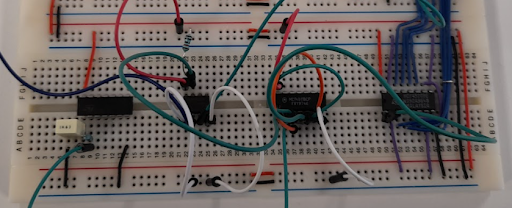
\includegraphics[width=0.9\textwidth]{images/comparatorTesting1.png}
        \caption{The comparator(2nd from left) \& NAND(3rd from left) chip setup before any test equipment attached}
        \label{fig:comparatorTesting1}
    \end{minipage}\hfill
    \begin{minipage}[t]{0.45\textwidth}
        \centering
        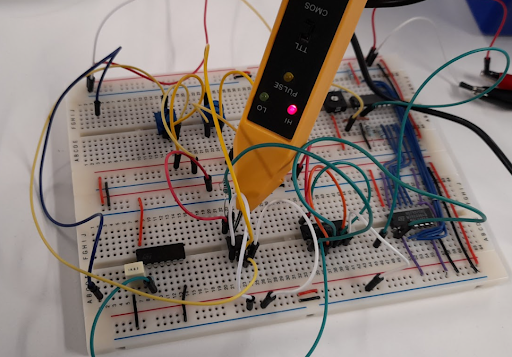
\includegraphics[width=0.9\textwidth]{images/comparatorTesting2.png}
        \caption{The comparator, rotary potentiometers and a logic probe showing a high output}
         \label{fig:comparatorTesting2}
    \end{minipage}
\end{figure}
\begin{figure} [H]
    \centering
    \begin{minipage}[t]{0.45\textwidth}
        \centering
        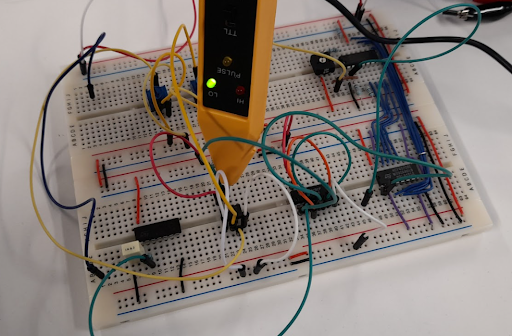
\includegraphics[width=0.9\textwidth]{images/comparatorTesting3.png}
        \caption{The comparator, rotary potentiometers and a logic probe showing a low output}
        \label{fig:comparatorTesting3}
    \end{minipage}\hfill
    \begin{minipage}[t]{0.45\textwidth}
        \centering
        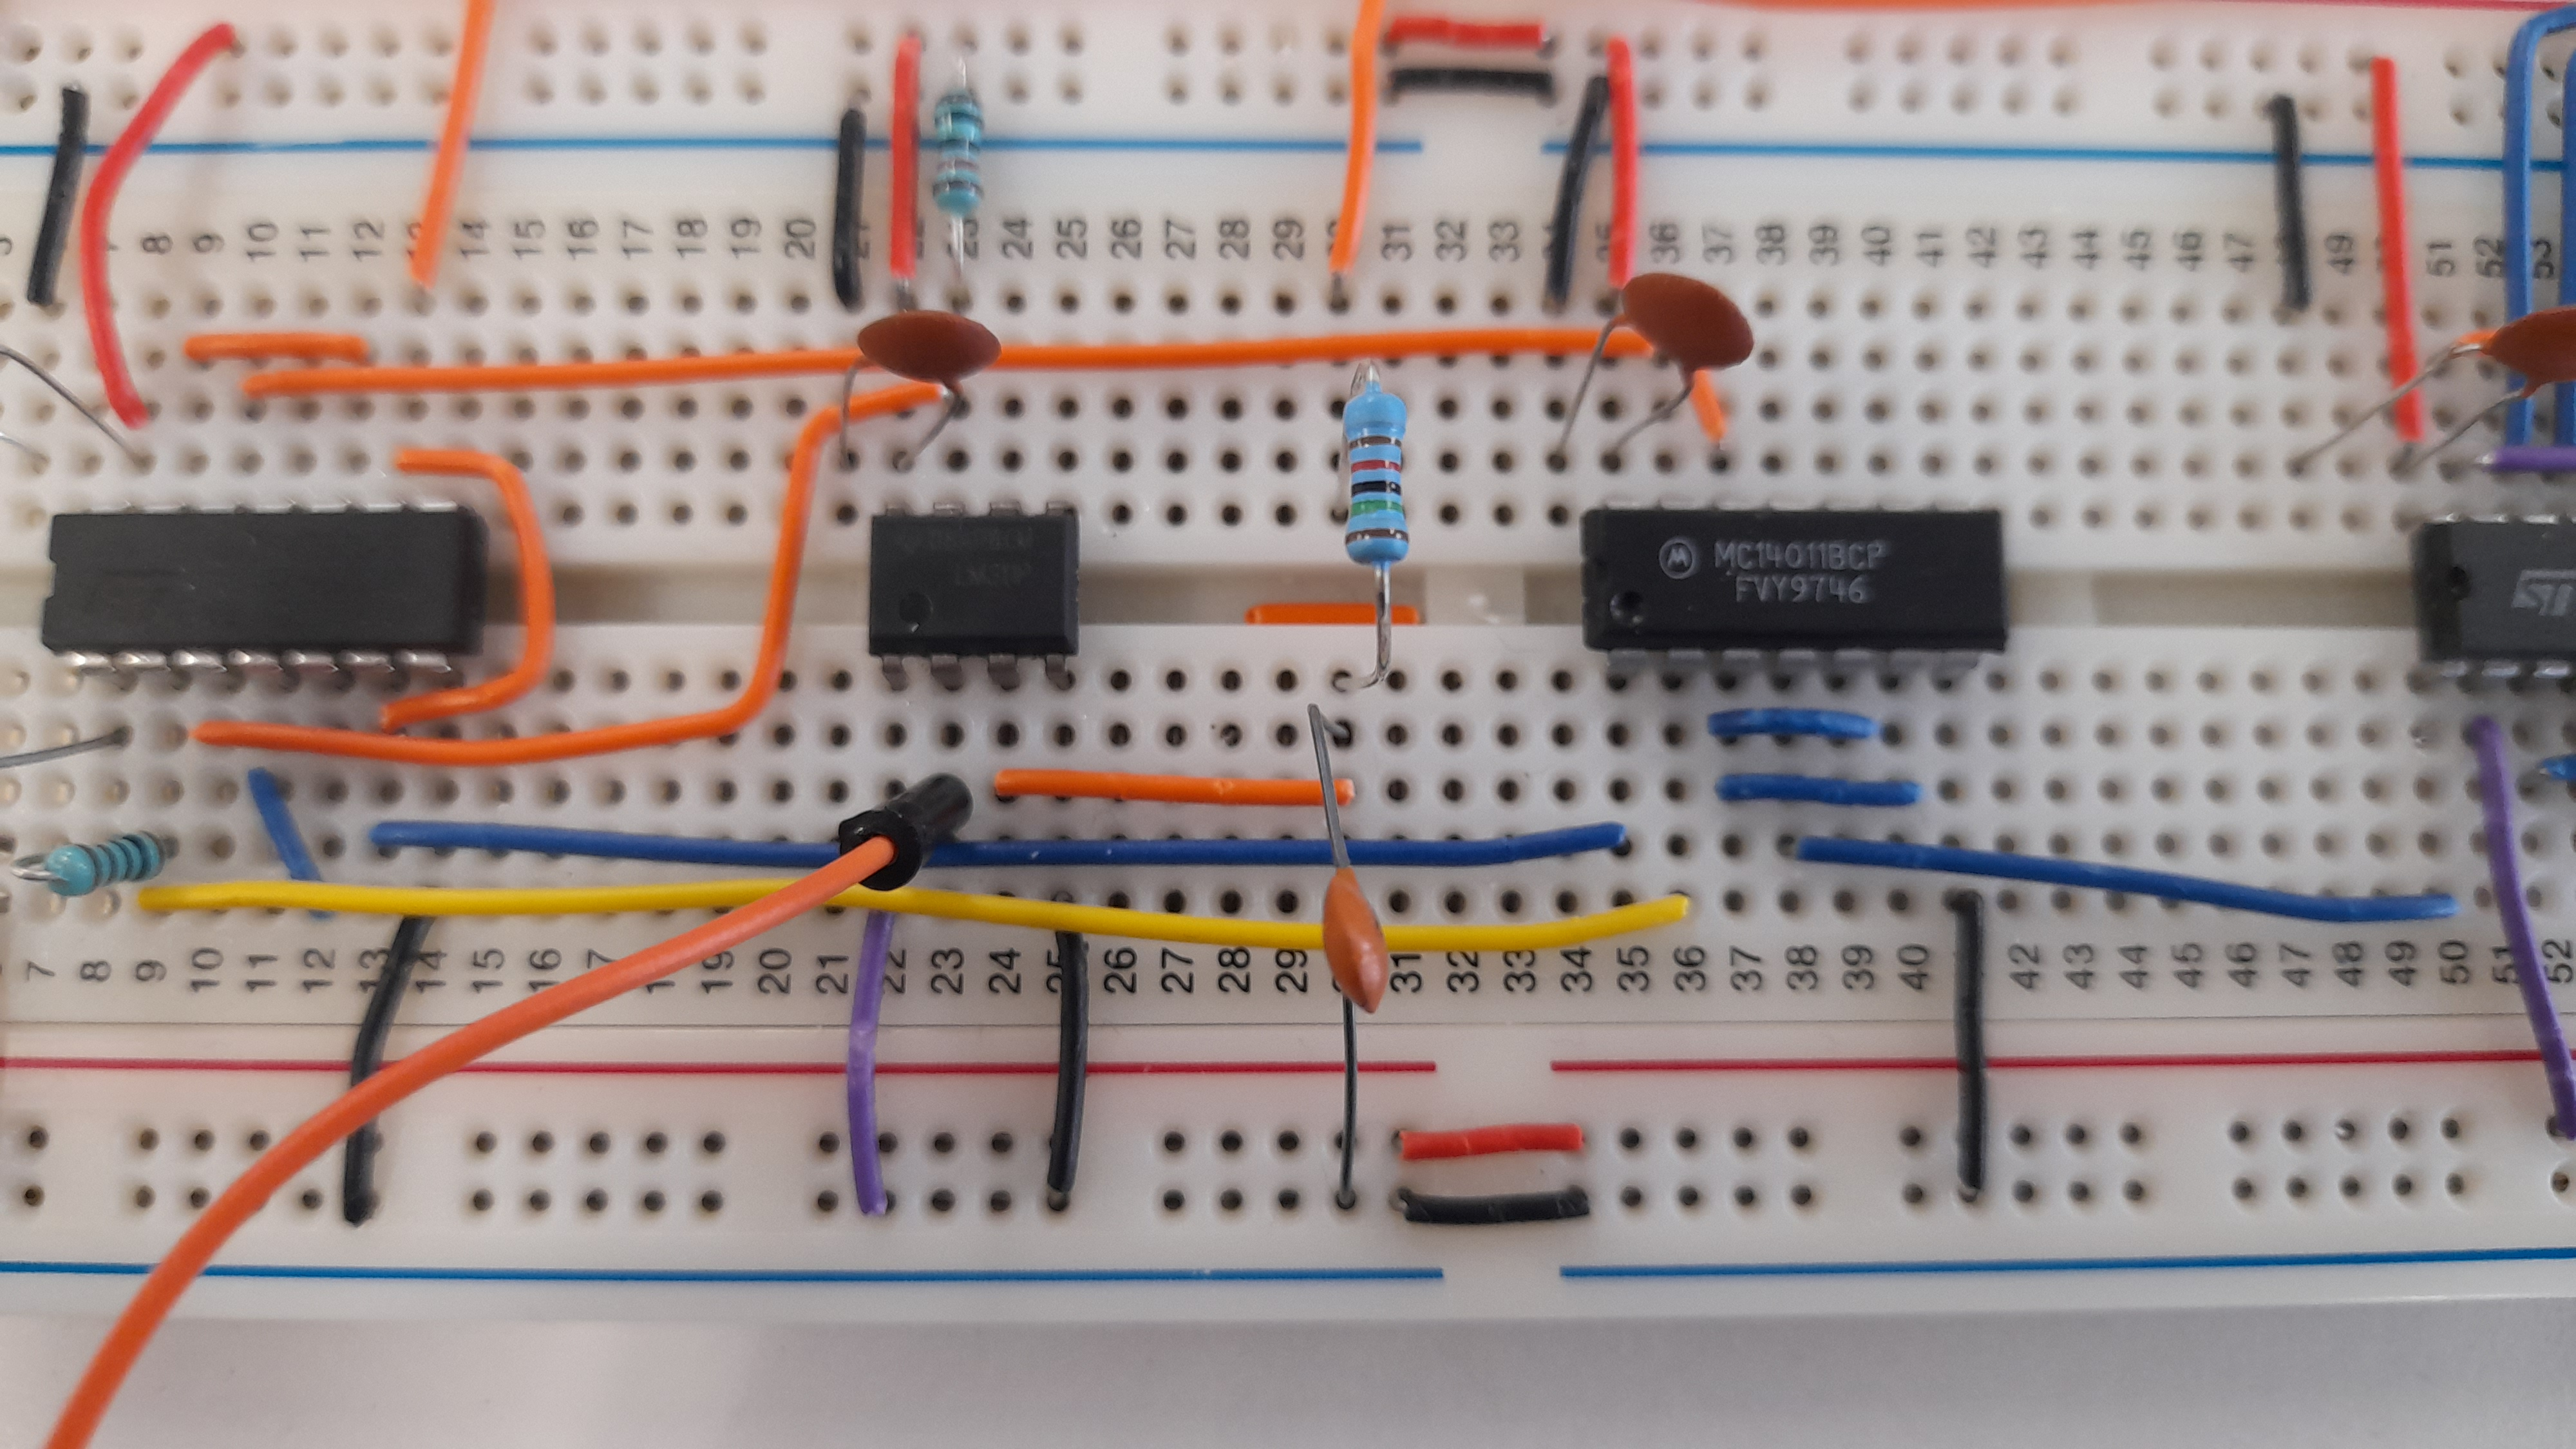
\includegraphics[width=0.9\textwidth]{images/comparatorNeatened.jpg}
        \caption{The neatened comparator subsystem (also shows LPF)}
        \label{fig:comparatorNeatened}
    \end{minipage}
\end{figure}
\noindent The output signal from the comparator wasn’t clean; this lead to false triggering of the reset to the counter. To resolve this, I put the signal through 2 Schmitt inverters to make the signal into more of a perfect logic 0 pulse. This worked and I was happy with the progress so far.

\begin{figure} [H]
    \centering
    \begin{minipage}[t]{0.45\textwidth}
        \centering
        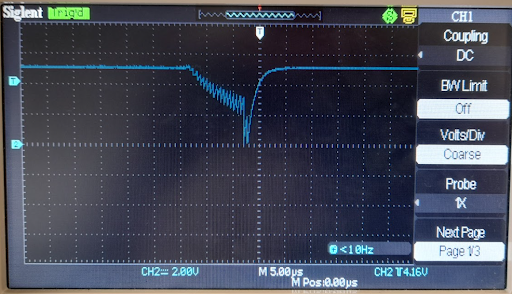
\includegraphics[width=0.9\textwidth]{images/comparatorTesting4.png}
        \caption{The comparator output before filtering with 2 Schmitt inverters}
        \label{fig:comparatorTesting4}
    \end{minipage}\hfill
    \begin{minipage}[t]{0.45\textwidth}
        \centering
        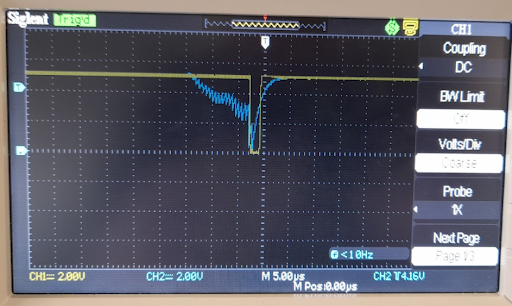
\includegraphics[width=0.9\textwidth]{images/comparatorTesting5.png}
        \caption{The before (blue) and after (yellow) filtering the comparator output with 2 Schmitt inverters}
         \label{fig:comparatorTesting5}
    \end{minipage}
\end{figure}

\subsection{Delay Line}
Delays are needed after the comparator has temporarily sent a low pulse to ensure that the correct things happen in the correct order. First the latches have to latch, then after some delay, the counter has to reset. It is important that these happen in this order so that the latches have latched before their signal is changed. 
\subsubsection{Design}
\begin{figure}[H]
    \centering
    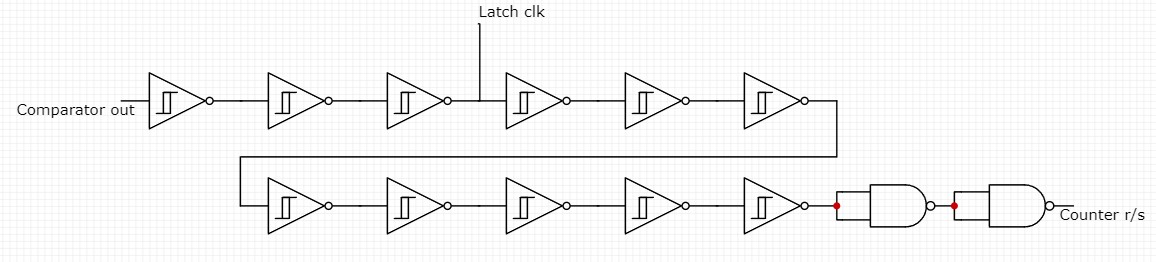
\includegraphics[width=0.9\textwidth]{images/delayCircuitDiagram.jpg}
    \caption{The circuit diagram for the delay line}
    \label{fig:delayCircuitDiagram}
\end{figure}
\subsubsection{Building \& Testing}
This delay line caused a lot of problems during the building and testing phase, especially during the construction of the latches. The final iteration of the design upon which I have settled, is by no means perfect, however it does work and the subsystems interact as I expect them to. It is not perfect as there is a seemingly unnecessary number of Schmitt inverters used, I discuss this and some possible solutions further in the testing and evaluation chapters. 

\subsection{Latch}
This will save the binary signal outputted from the counter when the correct value has been found. This signal will then be sent to the EEPROM.
\subsubsection{Design}
\begin{figure} [H]
    \centering
    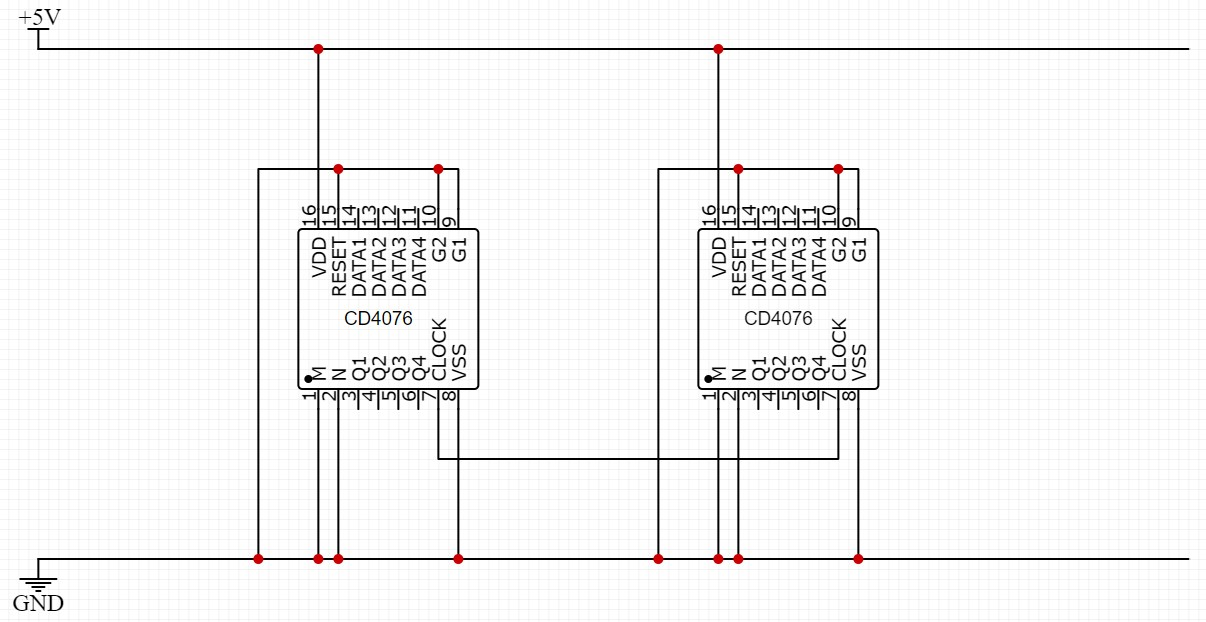
\includegraphics[width=0.6\textwidth]{images/latchCircuitDiagram.jpg}
    \caption{Circuit diagram of the latch}
    \label{fig:latchCircuitDiagram}
\end{figure}
\noindent Pins 3 through 6 inclusive for both chips will be connected to the EEPROM and pins 11 through 14 inclusive will be connected to the counter output lines. These have been omitted from this diagram for simplicity and can be seen in the full schematic.
\subsubsection{Building \& Testing}
I connected the latches as specified in my design. This didn’t work initially, so I troubleshooted and found that the noise on the output of the DAC was causing me problems. I then added the Low Pass Filter to that line which solved my problems. \textit{(See DAC design and testing for more information on this \& circuit diagram)}
\begin{figure} [H]
    \centering
    \begin{minipage}[t]{0.45\textwidth}
        \centering
        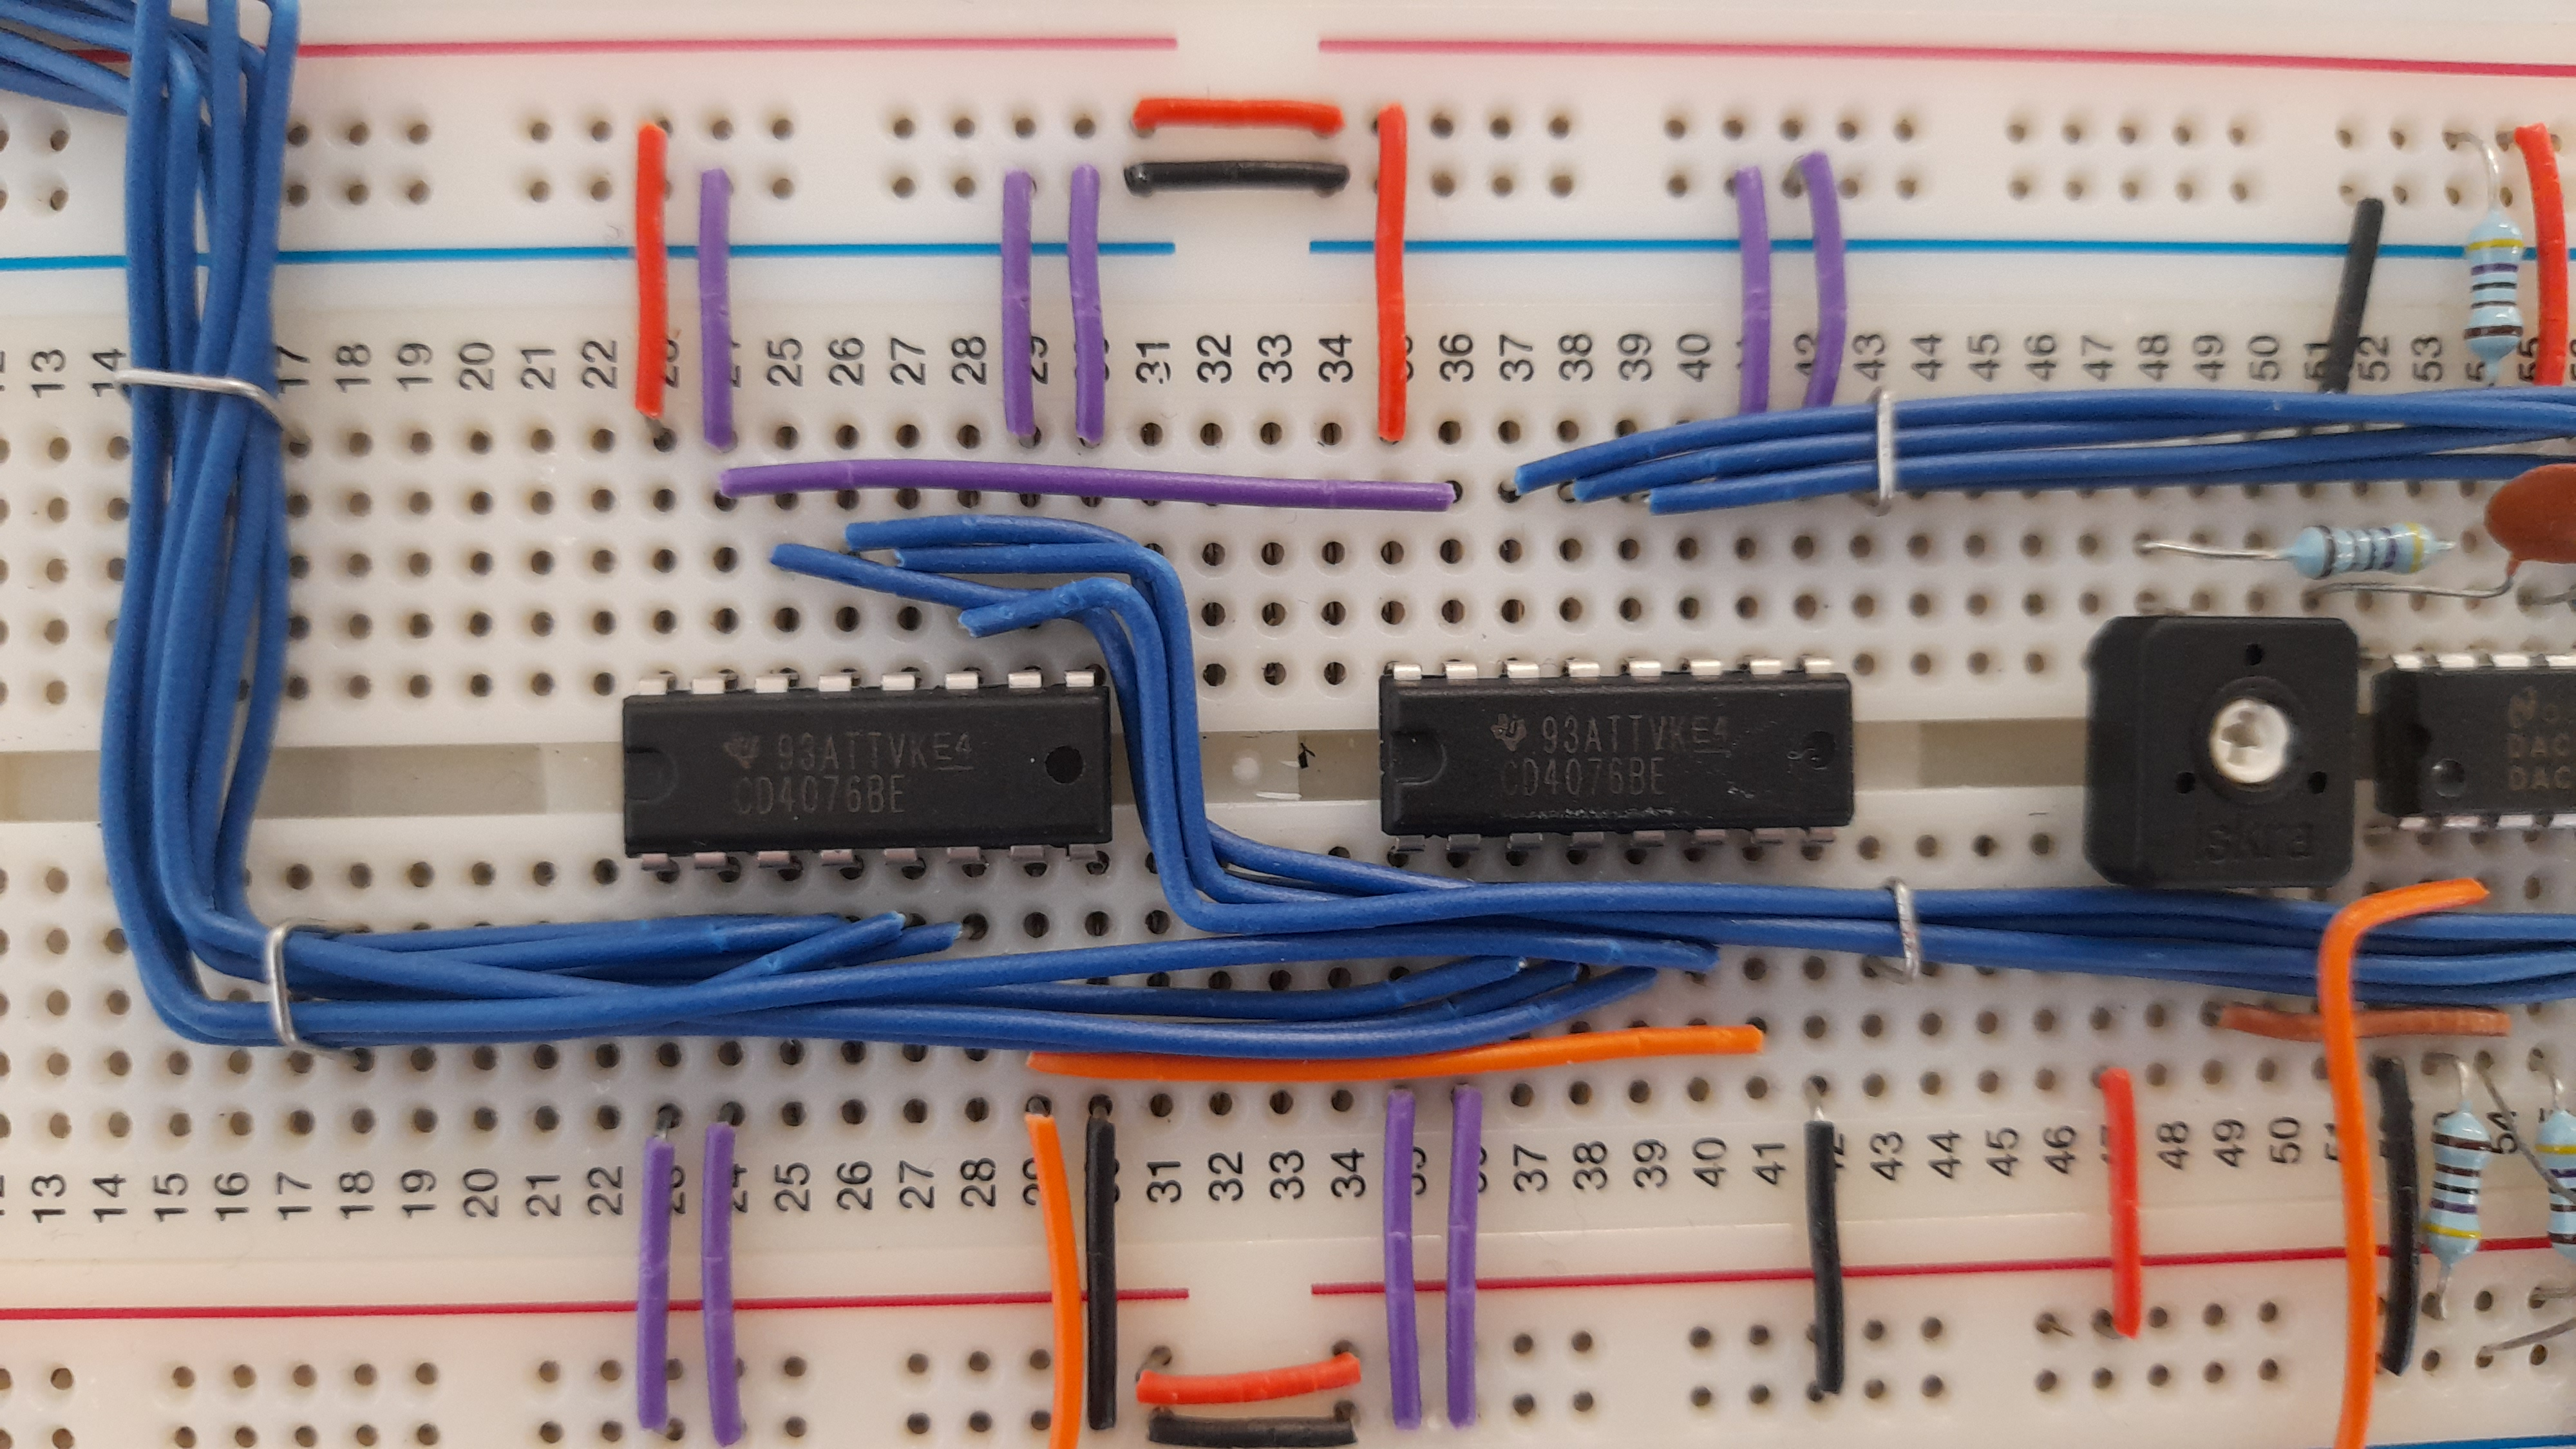
\includegraphics[width=0.9\textwidth]{images/latchNeatened.jpg}
        \caption{Neatened latch system}
        \label{fig:latchNeatened}
    \end{minipage}\hfill
    \begin{minipage}[t]{0.45\textwidth}
        \centering
    \end{minipage}
\end{figure}

\subsection{Low Pass Filter}
\label{sec:LPF}
This subsystem is needed to filter out the noise from the output of the DAC. The DAC's output has a frequency of about 4MHz which is extremely high. The break frequency I will be using is 10KHz, this should be high enough to still allow the ramp waveform through.
\subsubsection{Design}
I first drew the circuit diagram for this circuit.
\begin{figure}[H]
    \centering
    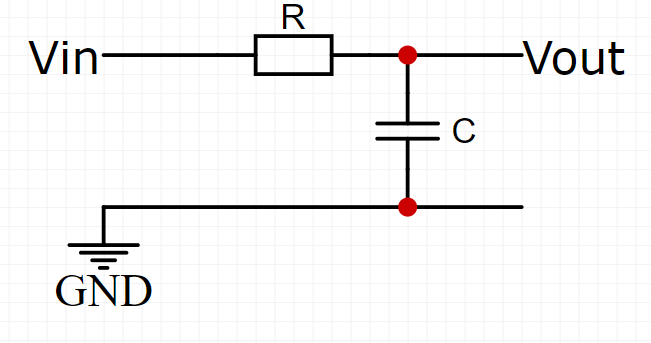
\includegraphics[width=7.5cm]{images/lpfCircuitDiagram.PNG}
    \caption{The circuit Diagram for the low pass filter}
    \label{fig:lpfCircuitDiagram}
\end{figure}
\noindent I then calculated the values for the resistor and capacitor using the break frequency formula with a break frequency of 10KHz.\newline
$\displaystyle f_b = \frac{1}{2 \pi RC}$ \vspace{3mm} \newline
$\displaystyle 10\times 10 ^3 = \frac{1}{2 \pi RC}$ \vspace{3mm} \newline
$\displaystyle R = \frac{1}{2\pi(10\times 10 ^3)C}$ \vspace{3mm} \newline
$\displaystyle R = \frac{1}{2\pi(10\times 10 ^3)(10\times 1 ^{-9})}$ \vspace{3mm} \newline
$R = 15915.49431\Omega$ \vspace{3mm} \newline
$R\approx 1.59K\Omega$ \vspace{3mm} \newline
This means the resultant component values are: \newline
\indent $R = 16K\Omega$ \newline
\indent $C = 1nF$
\subsubsection{Building \& Testing}
I built this as I had specified in my design. This worked extremely well; reducing the amount of noise on the analogue output of the DAC.
\begin{figure} [H]
    \centering
    \begin{minipage}[t]{0.45\textwidth}
        \centering
        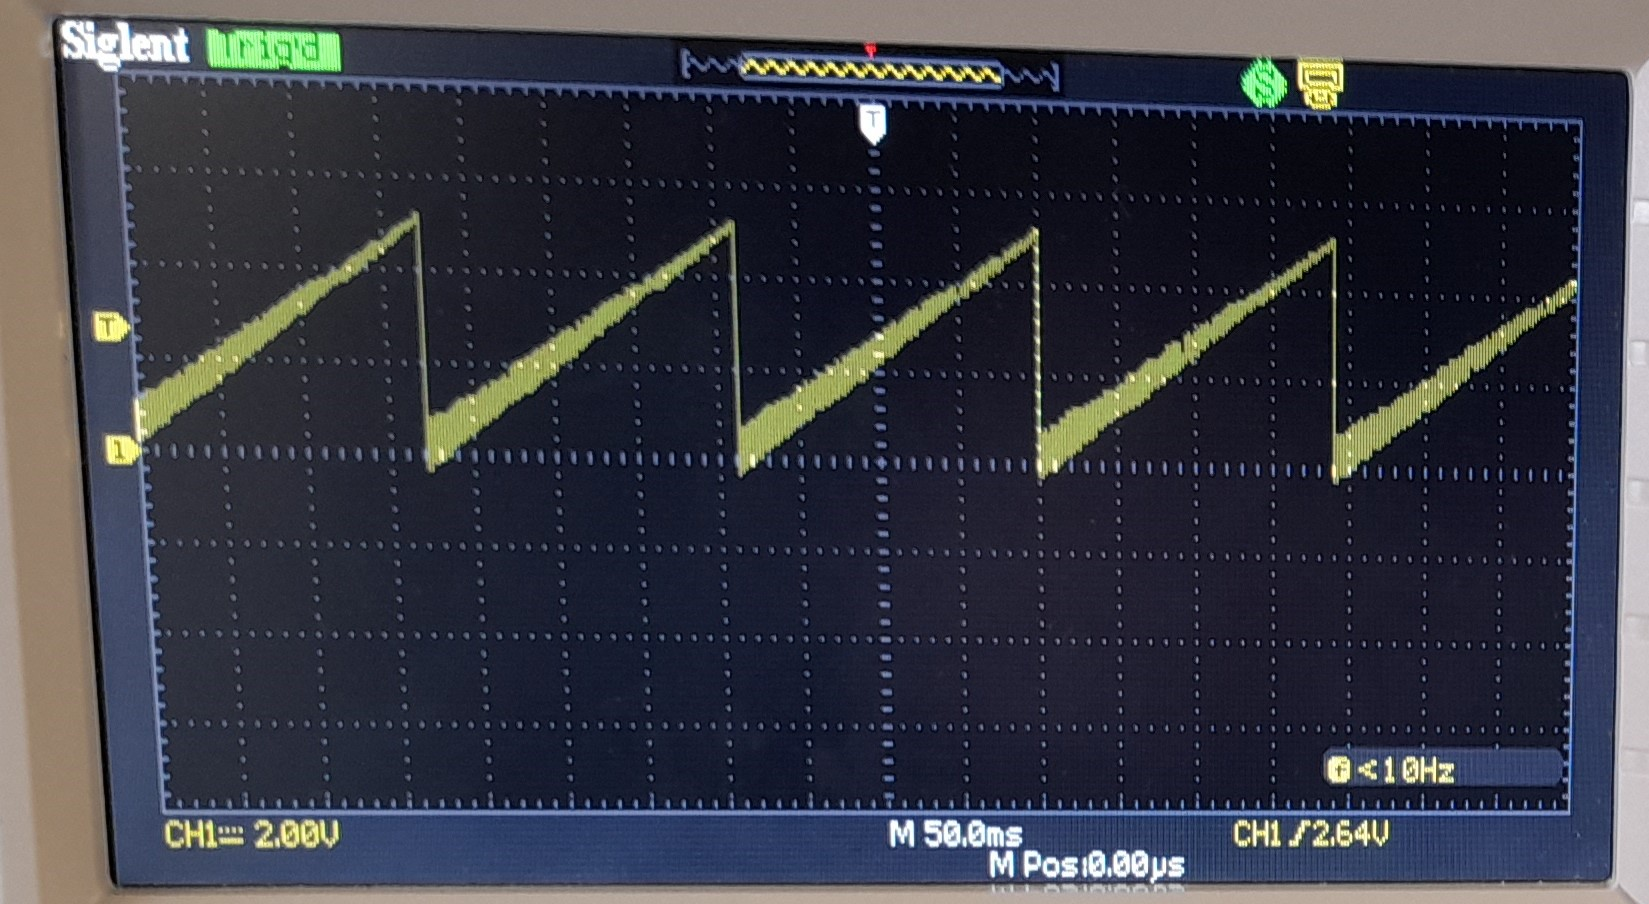
\includegraphics[width=0.9\textwidth]{images/lpfInputZoomed.jpg}
        \caption{The input to the Low Pass Filter}
        \label{fig:lpfInput}
    \end{minipage}\hfill
    \begin{minipage}[t]{0.45\textwidth}
        \centering
        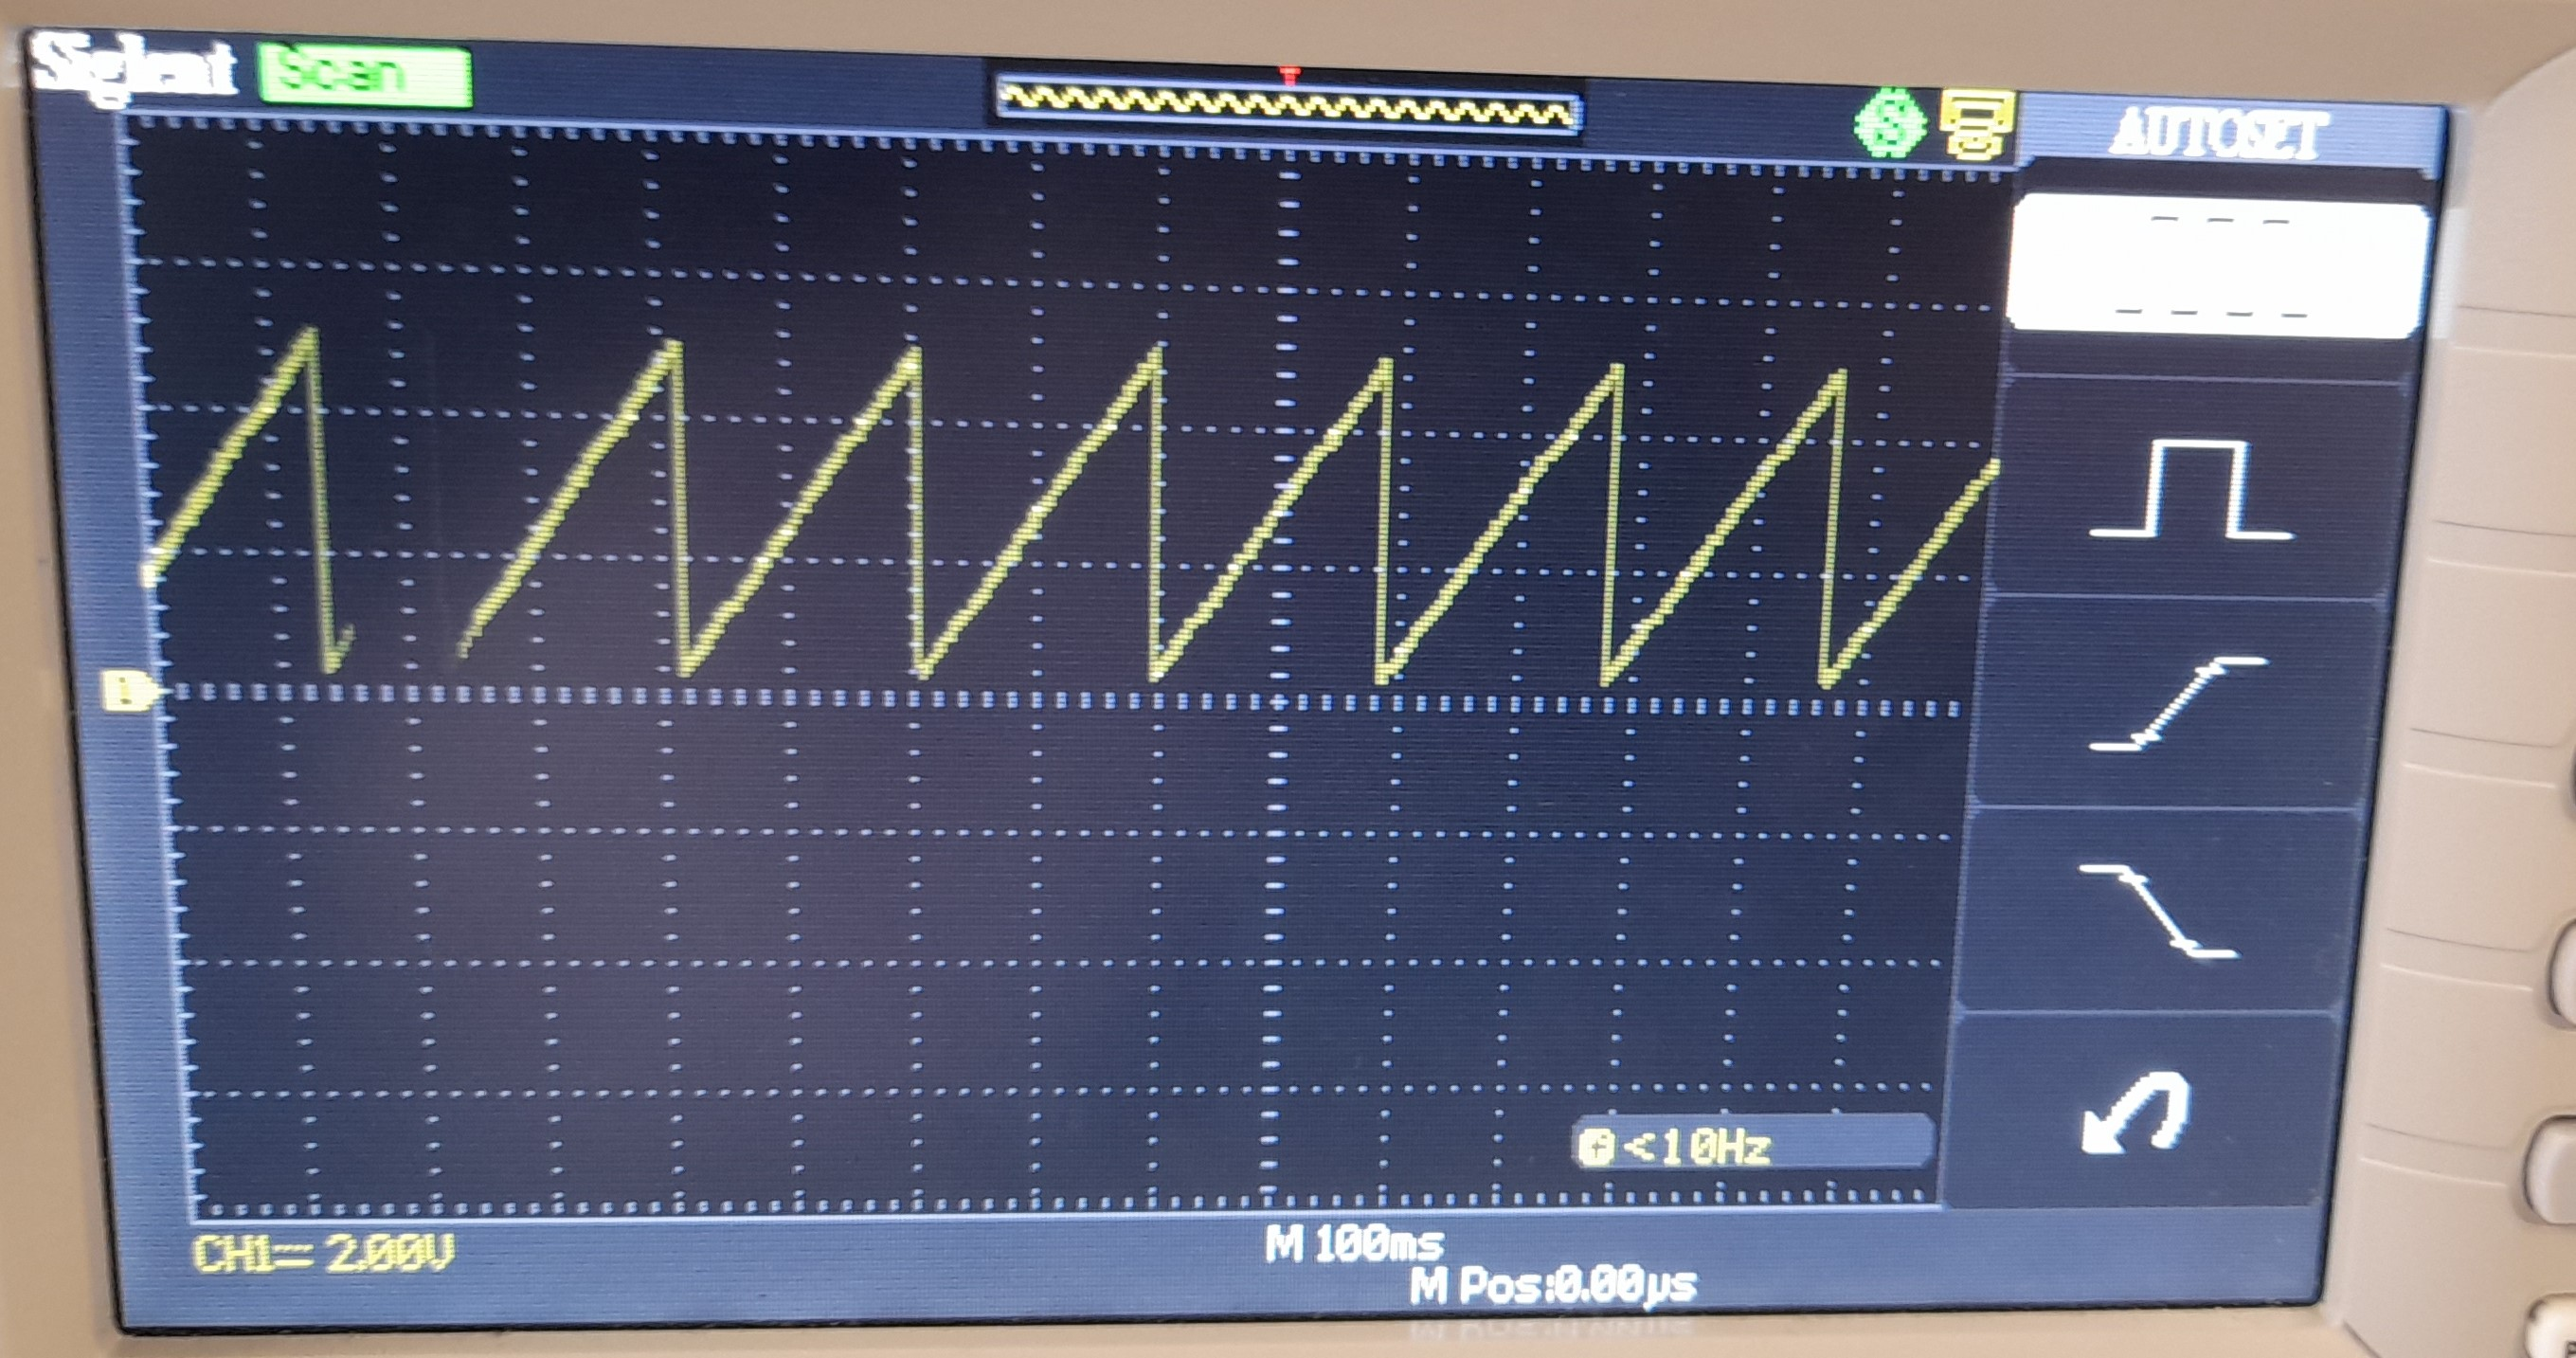
\includegraphics[width=0.9\textwidth]{images/lpfOutputZoomed.jpg}
        \caption{The output of the Low Pass Filter}
         \label{fig:lpfOutput}
    \end{minipage}
\end{figure}
\begin{figure} [H]
    \centering
    \begin{minipage}[t]{0.45\textwidth}
        \centering
        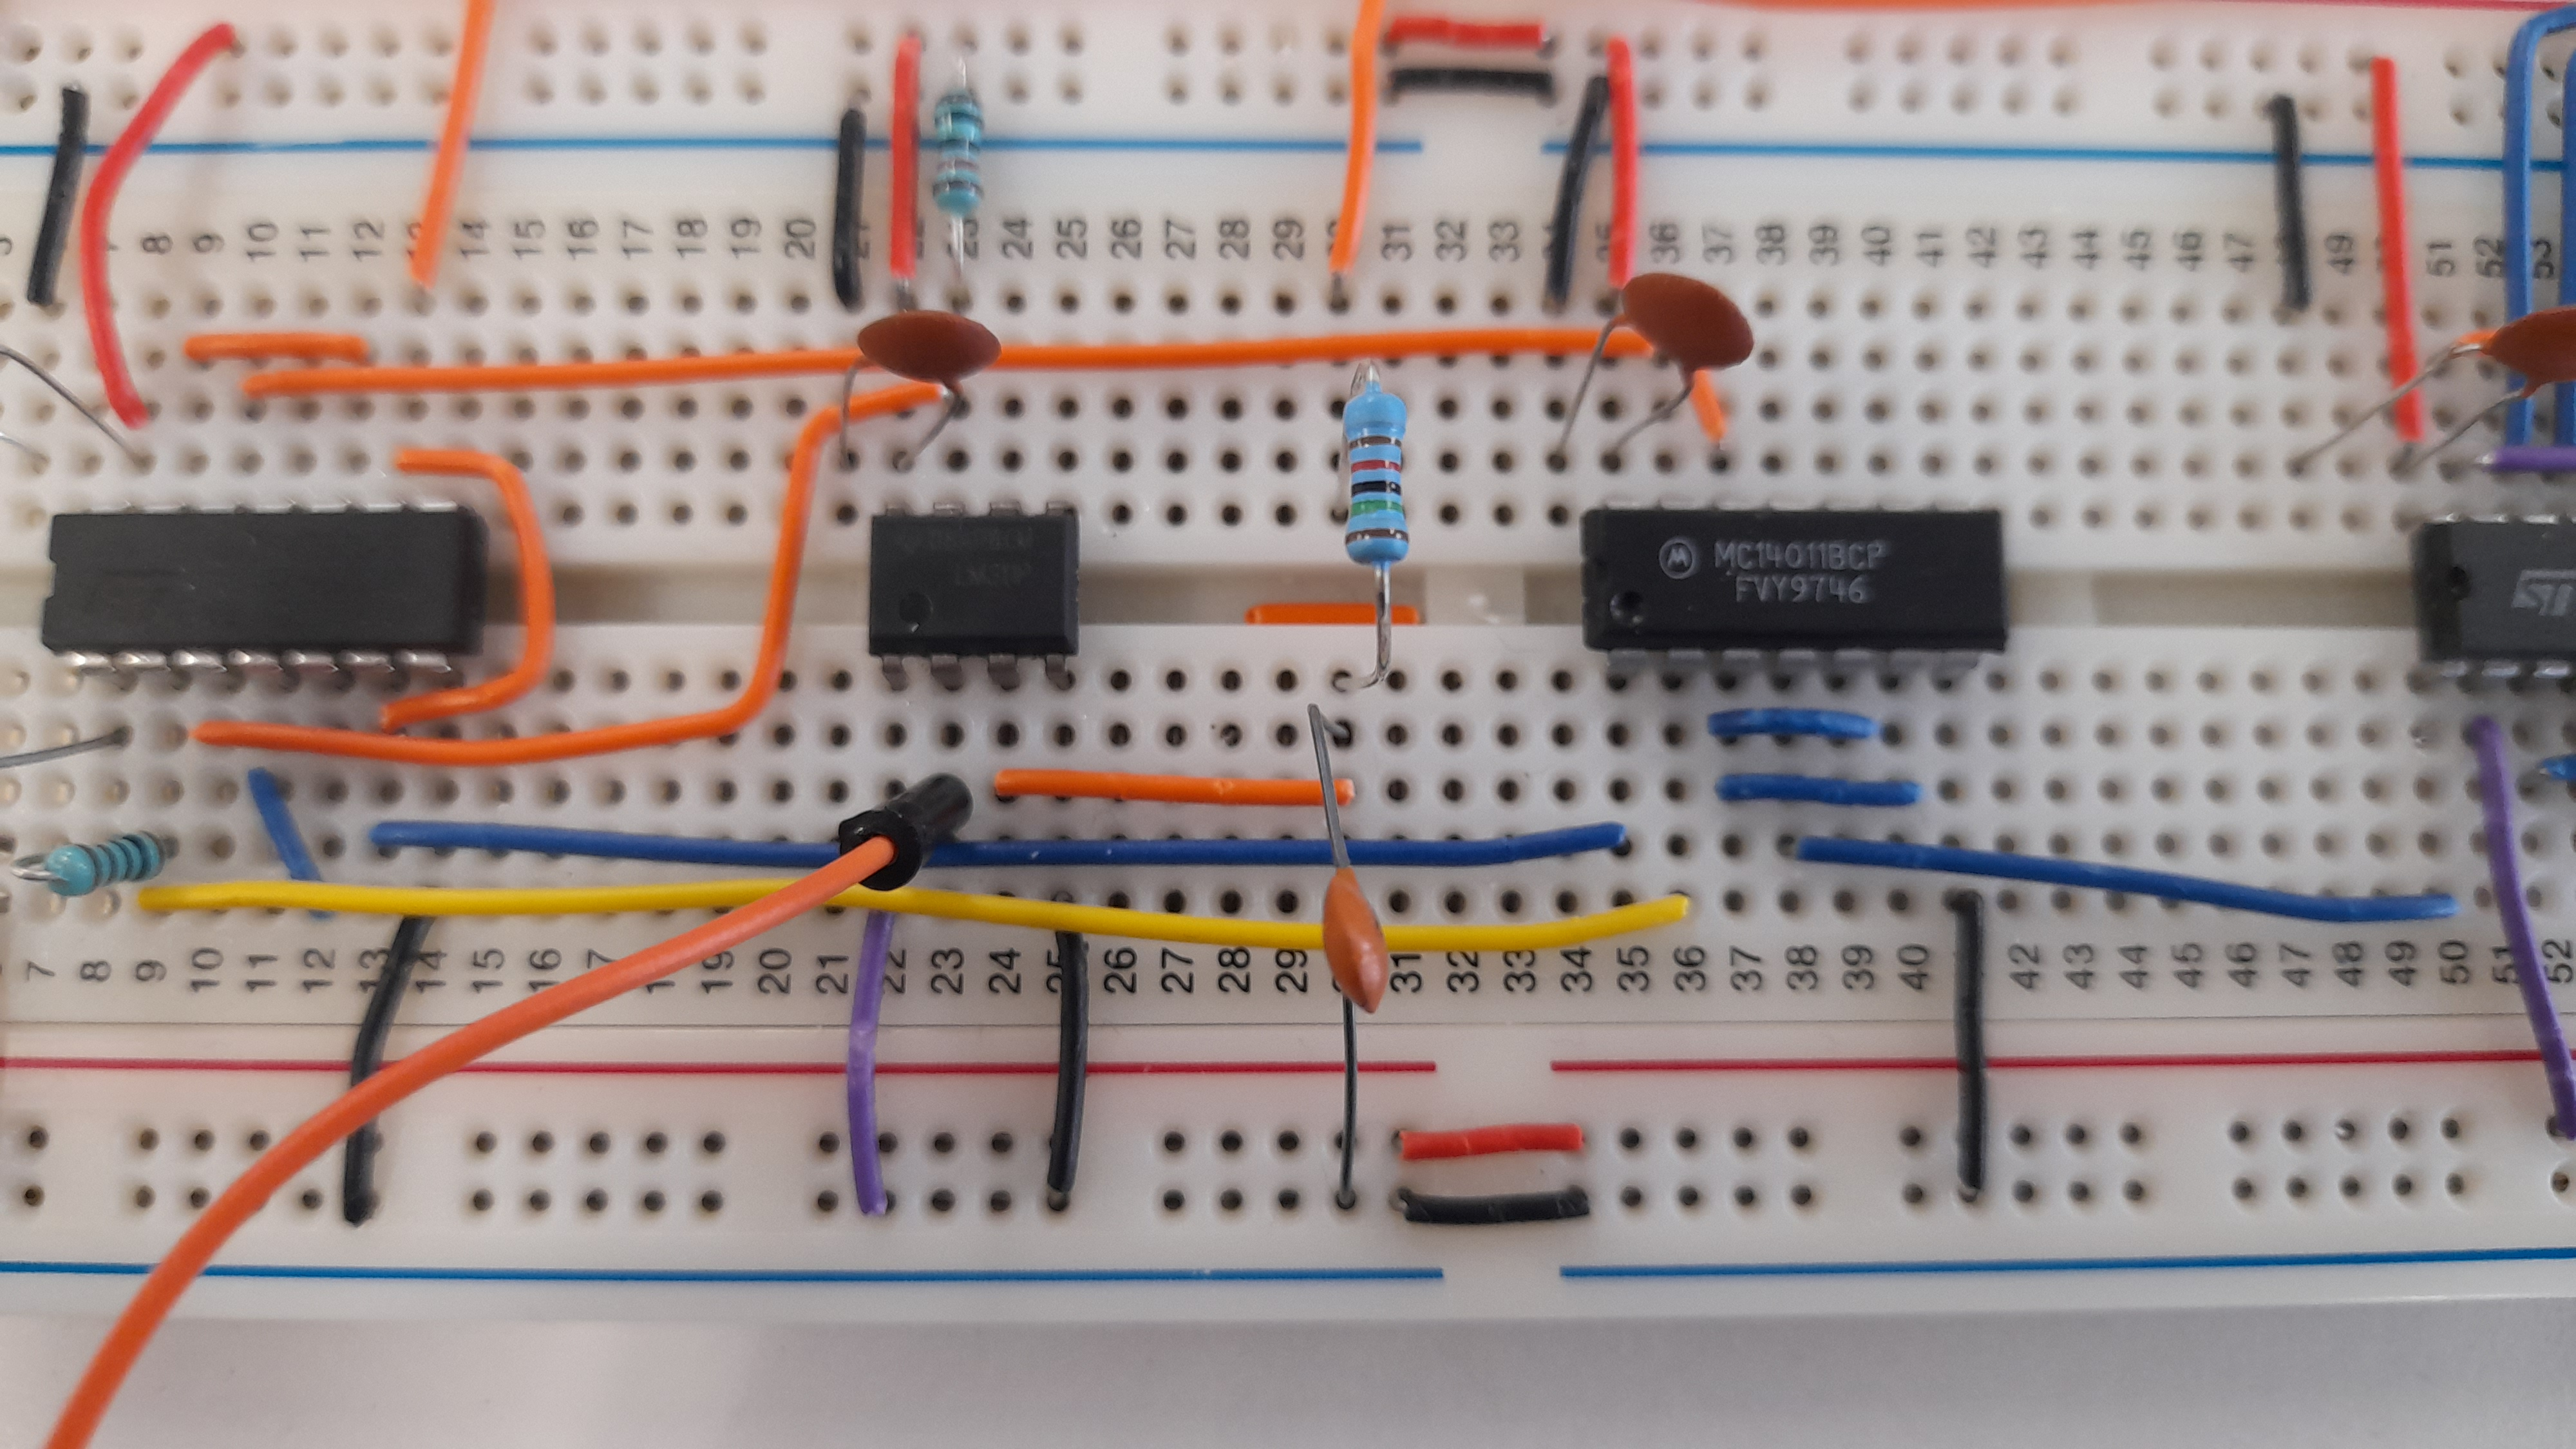
\includegraphics[width=0.9\textwidth]{images/comparatorNeatened.jpg}
        \caption{The physical layout of the Low Pass Filter on the breadboard}
        \label{fig:lpfPhysical}
    \end{minipage}\hfill
    \begin{minipage}[t]{0.45\textwidth}
        \centering
    \end{minipage}
\end{figure}

\noindent An alternative subsystem I could have used is an active filter, this would have increased the complexity however as it would require an additional resistor and op-amp. Alternatively, I could have used a band pass filter, however this would also require an additional component - the inductor. Both of these options would have added unnecessary complexity as the simple passive low pass filter works fine.

\section{Display Subsystem}
There will be two seven-segment displays, one for the units and one for the tenths. The one for the units will have a decimal point which will be permanently tied high.
\subsubsection{Design}
\begin{figure}[H]
    \centering
    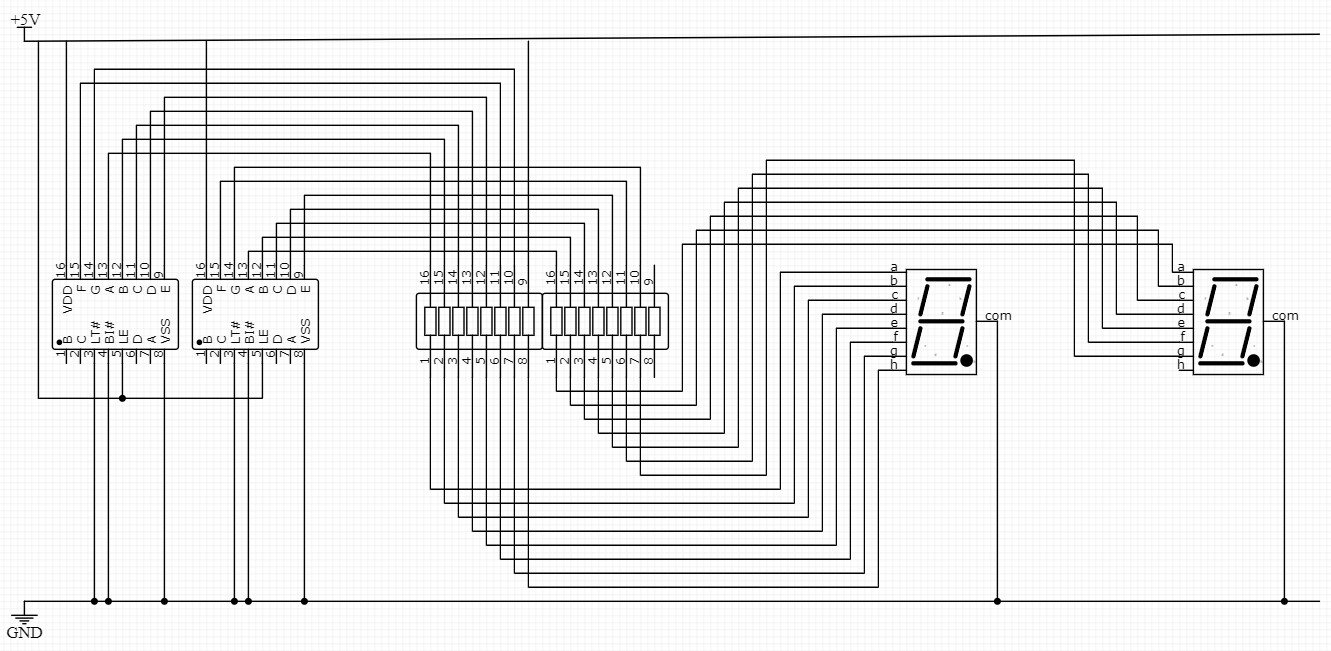
\includegraphics[width=0.9\textwidth]{images/displayCircuitDiagram.jpg}
    \caption{The circuit diagram for the display subsystem}
    \label{fig:displayCircuitDiagram}
\end{figure}
The inputs A, B, C and D for each of the display drivers will be connected to the outputs of the EEPROM. These connections can be seen in the full circuit diagram in the appendix.

\subsubsection{Building \& Testing}
First I connected this up as specified in my design, except from pins 3, 4 and 5 which I left unconnected. After I had connected these, the design worked. To confirm that the design worked, I fed a binary signal into the display subsystem. This can be seen in Figures \ref{fig:displayTesting1} \& \ref{fig:displayTesting2}.\newline
\begin{figure} [H]
    \centering
    \begin{minipage}[t]{0.45\textwidth}
        \centering
        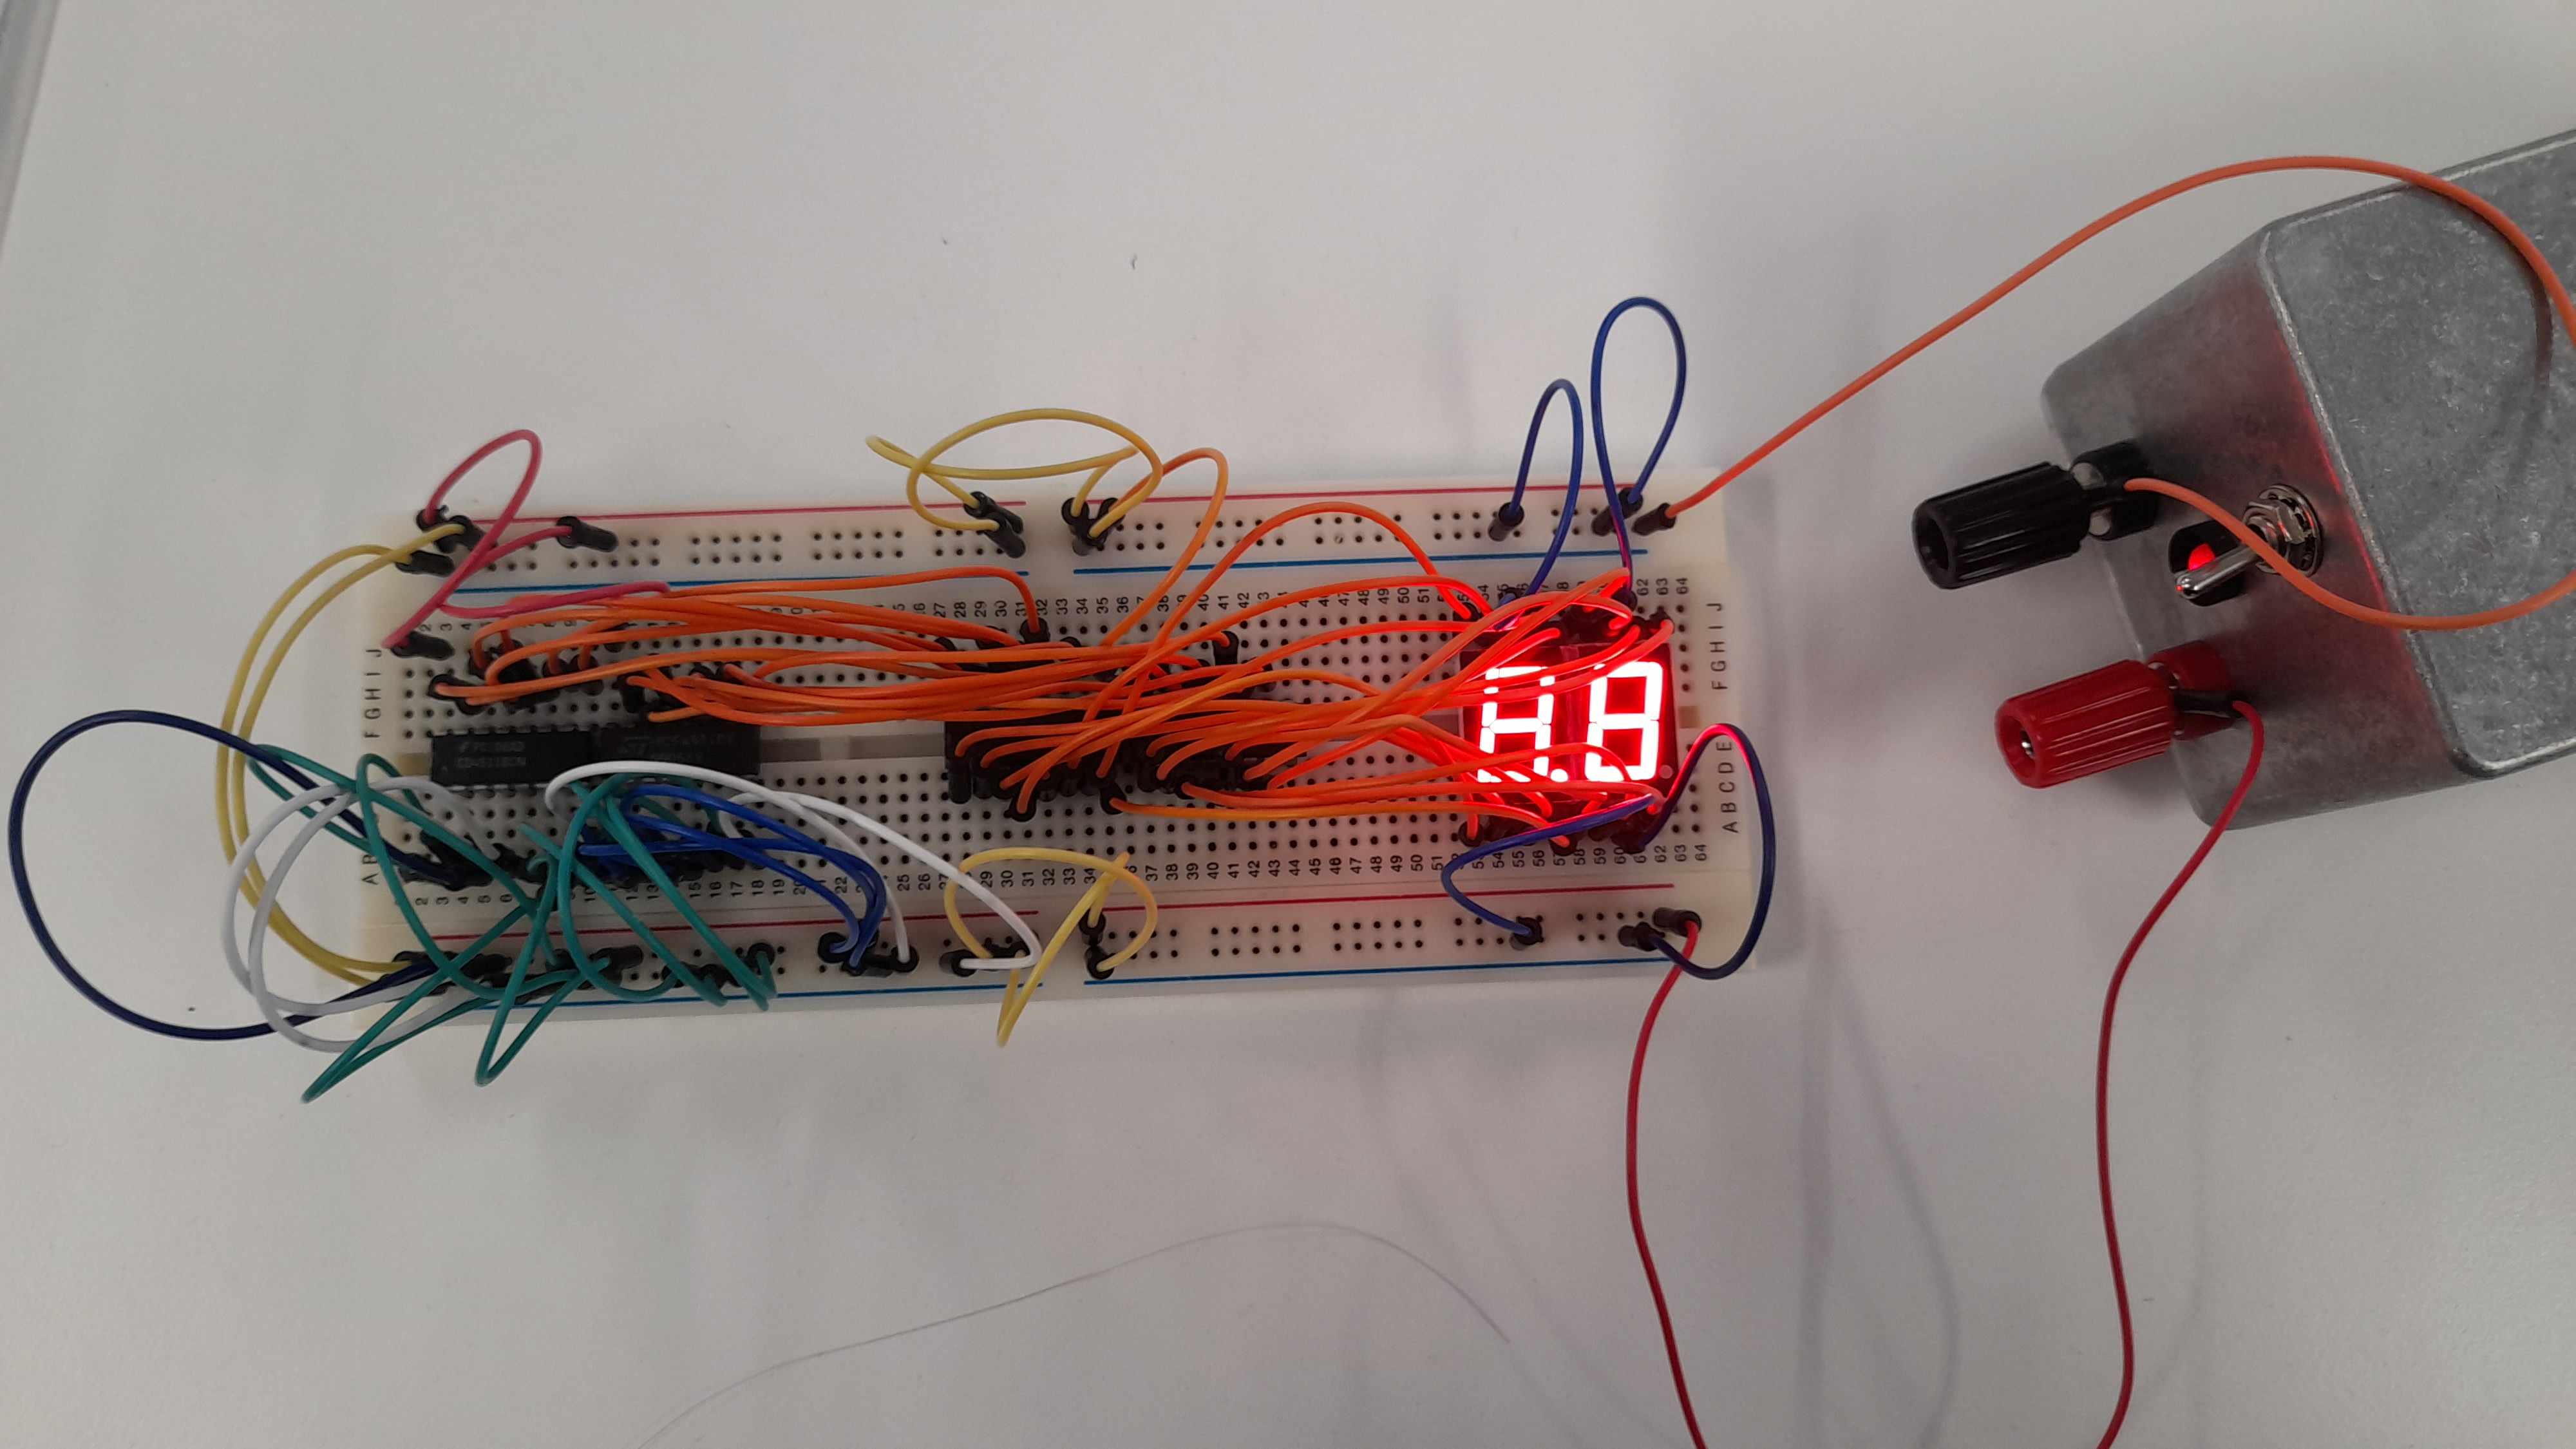
\includegraphics[width=0.9\textwidth]{images/displayTesting1.jpg}
        \caption{Pre-neatened subsystem showing 8.8}
        \label{fig:displayTesting1}
    \end{minipage}\hfill
    \begin{minipage}[t] {0.45\textwidth}
        \centering
        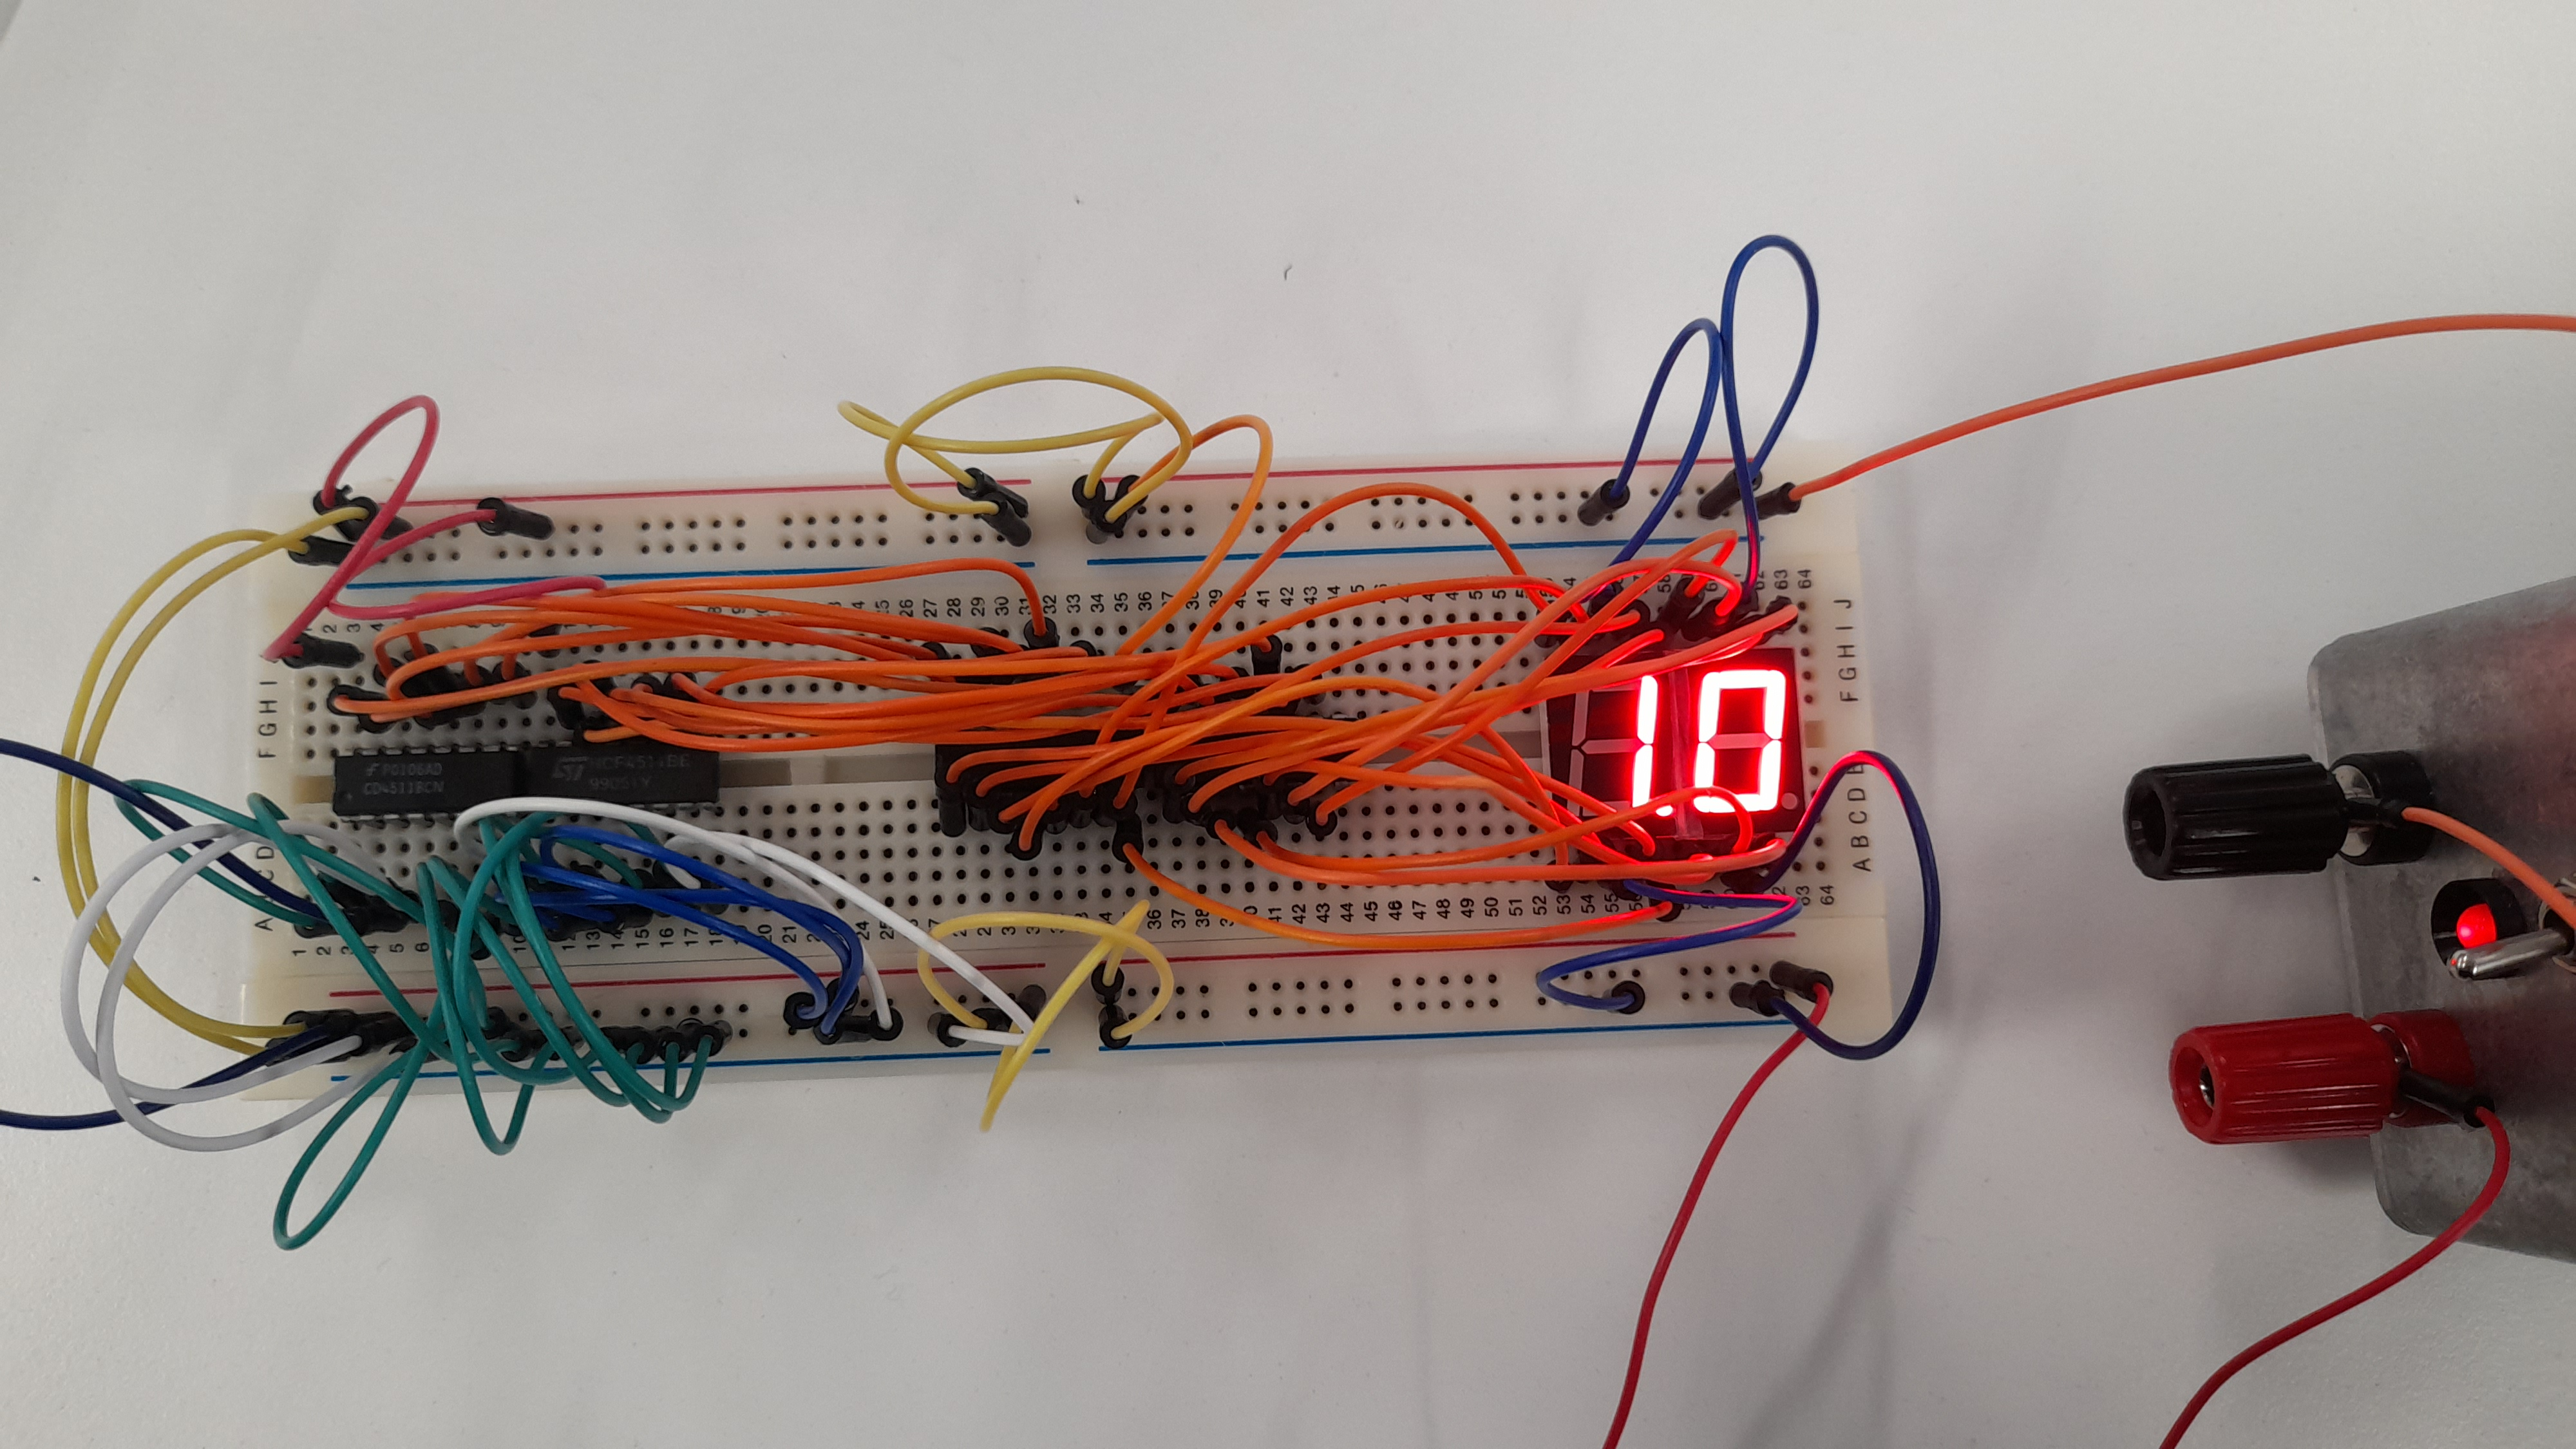
\includegraphics[width=0.9\textwidth]{images/displayTesting2.jpg}
        \caption{Pre-neatened subsystem showing 1.0}
         \label{fig:displayTesting2}
    \end{minipage}
\end{figure}
\noindent I then neatened the subsystem. To test that I hadn't broken anything during the neatening process, I used temporary jumper wires to act as the bits being fed into the display drivers. During testing, I found that I hadn't broken anything and the subsystem was working as I wanted it to.
\begin{figure} [H]
    \centering
    \begin{minipage}[t]{0.45\textwidth}
        \centering
        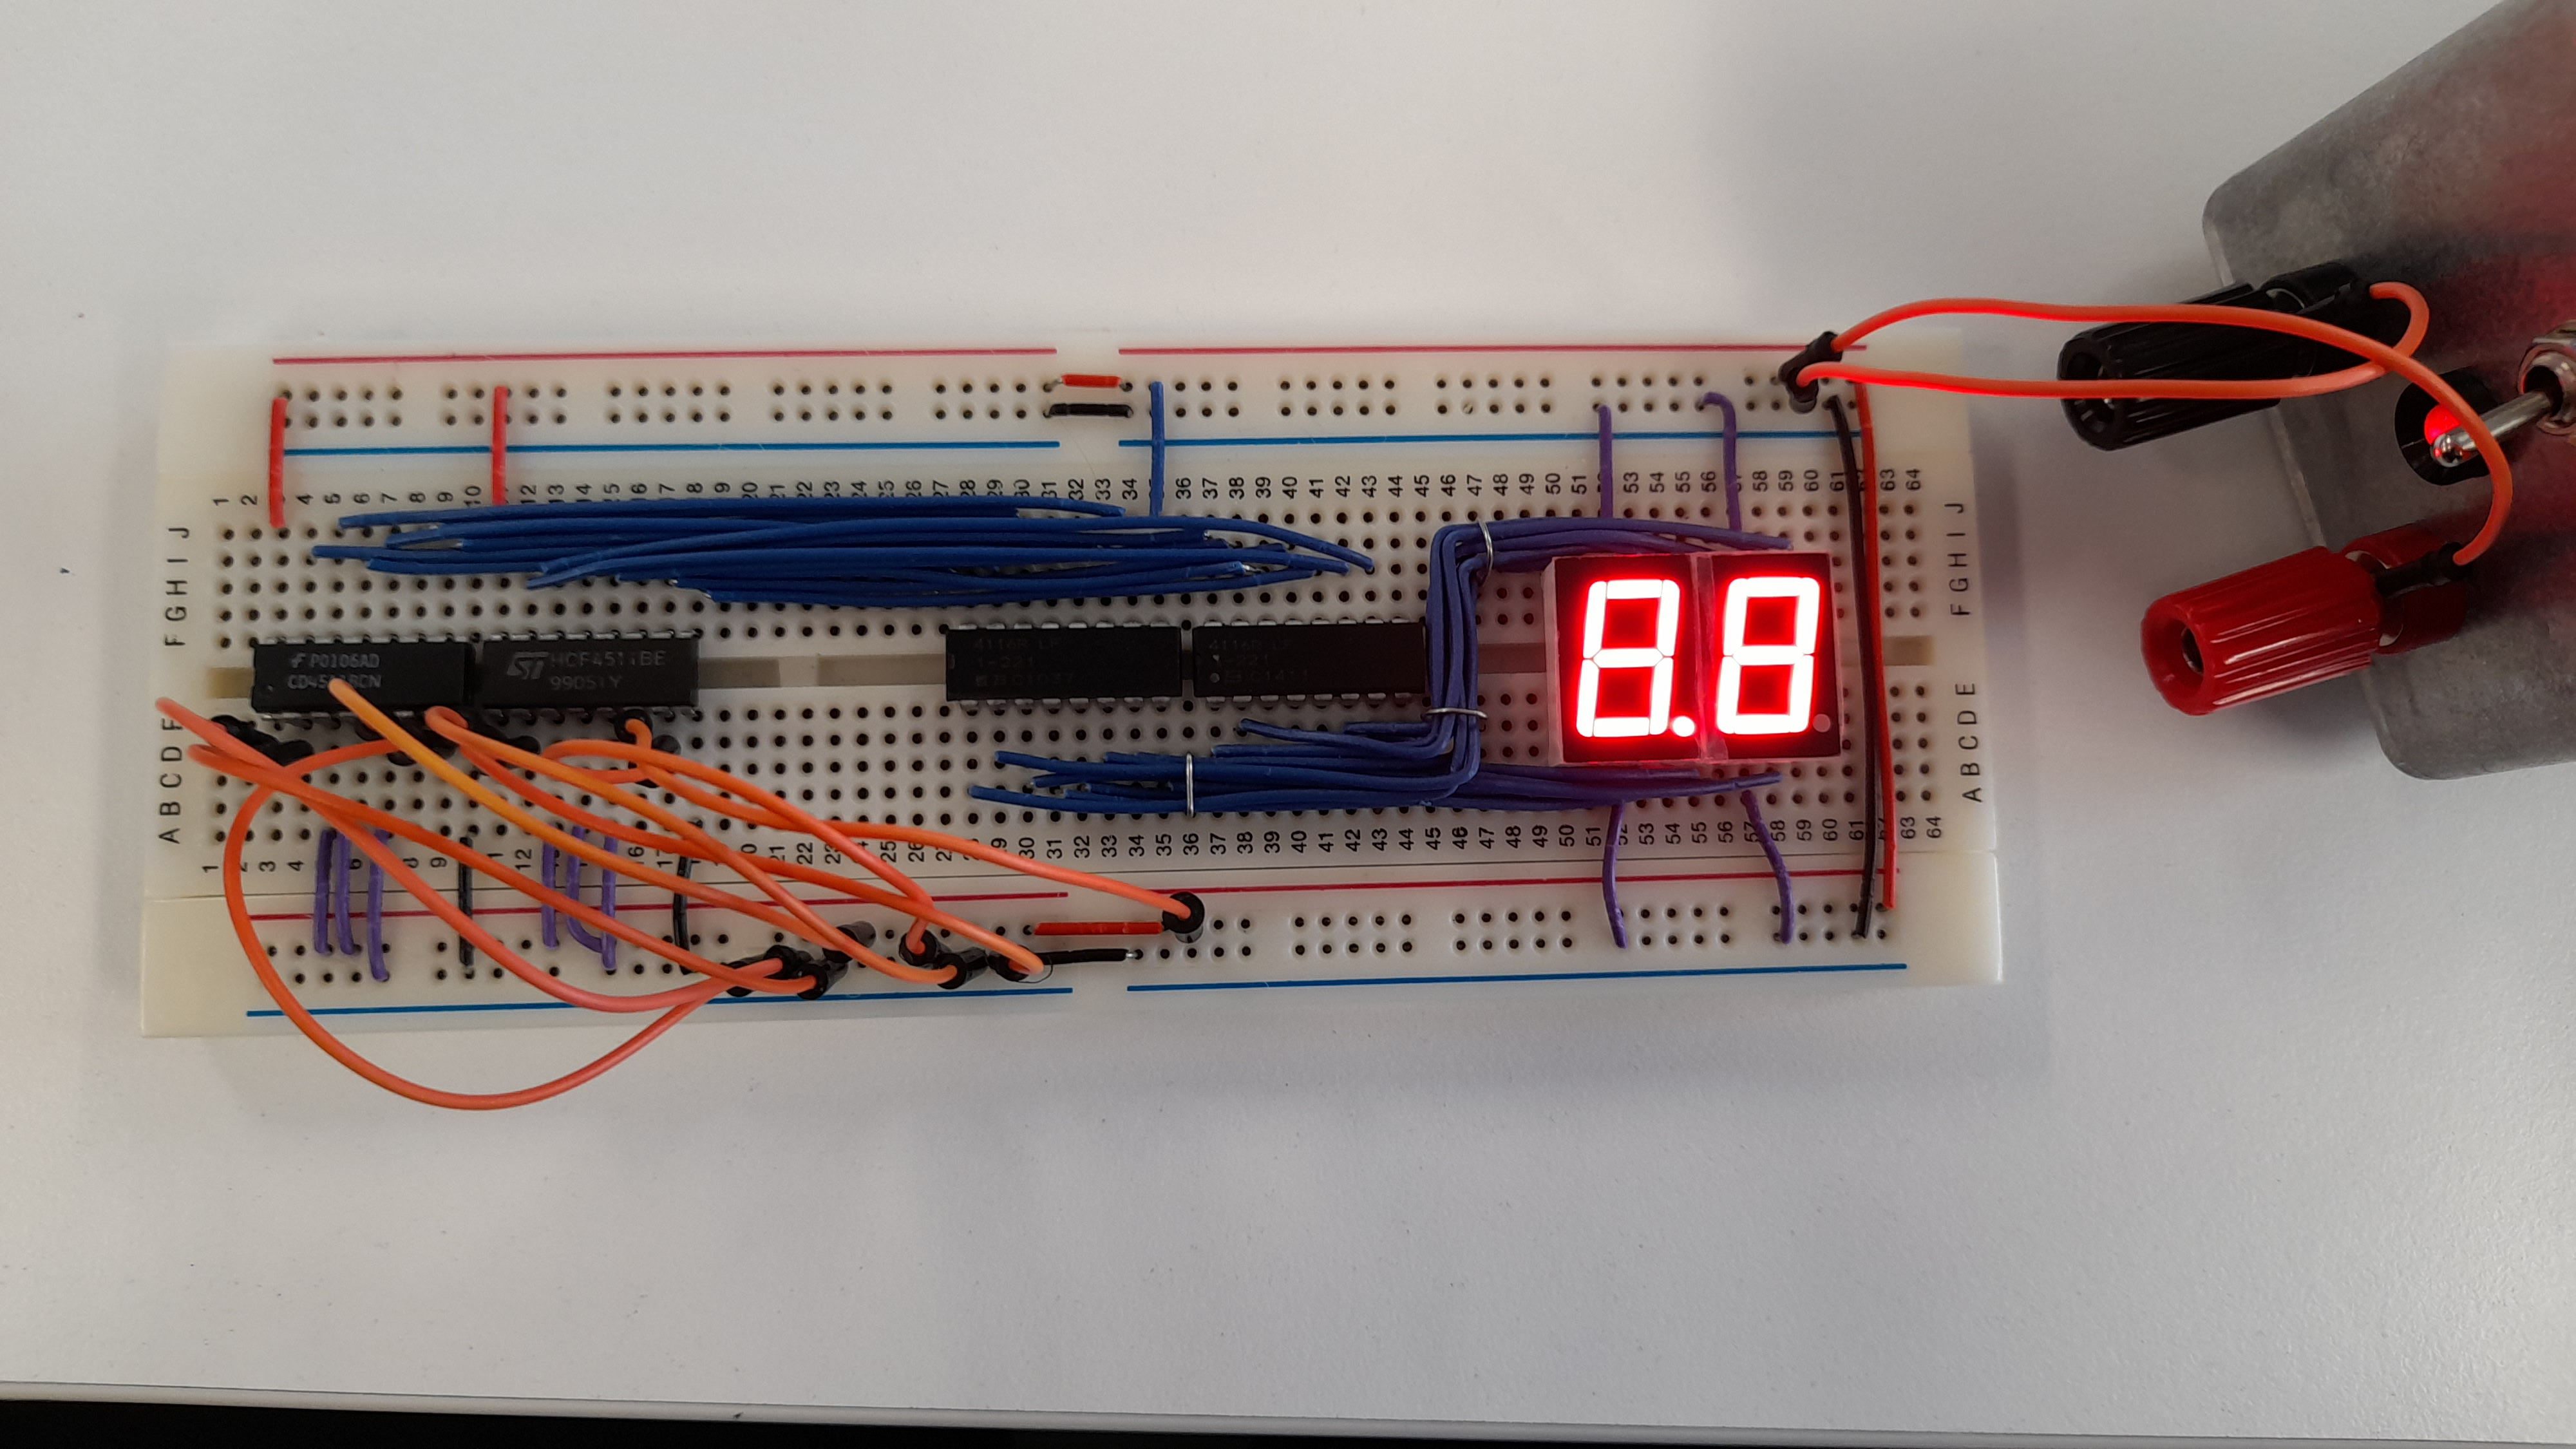
\includegraphics[width=0.9\textwidth]{images/displayTesting3.jpg}
        \caption{Neatened subsystem showing 8.8}
        \label{fig:displayTesting3}
    \end{minipage}\hfill
    \begin{minipage}[t] {0.45\textwidth}
        \centering
        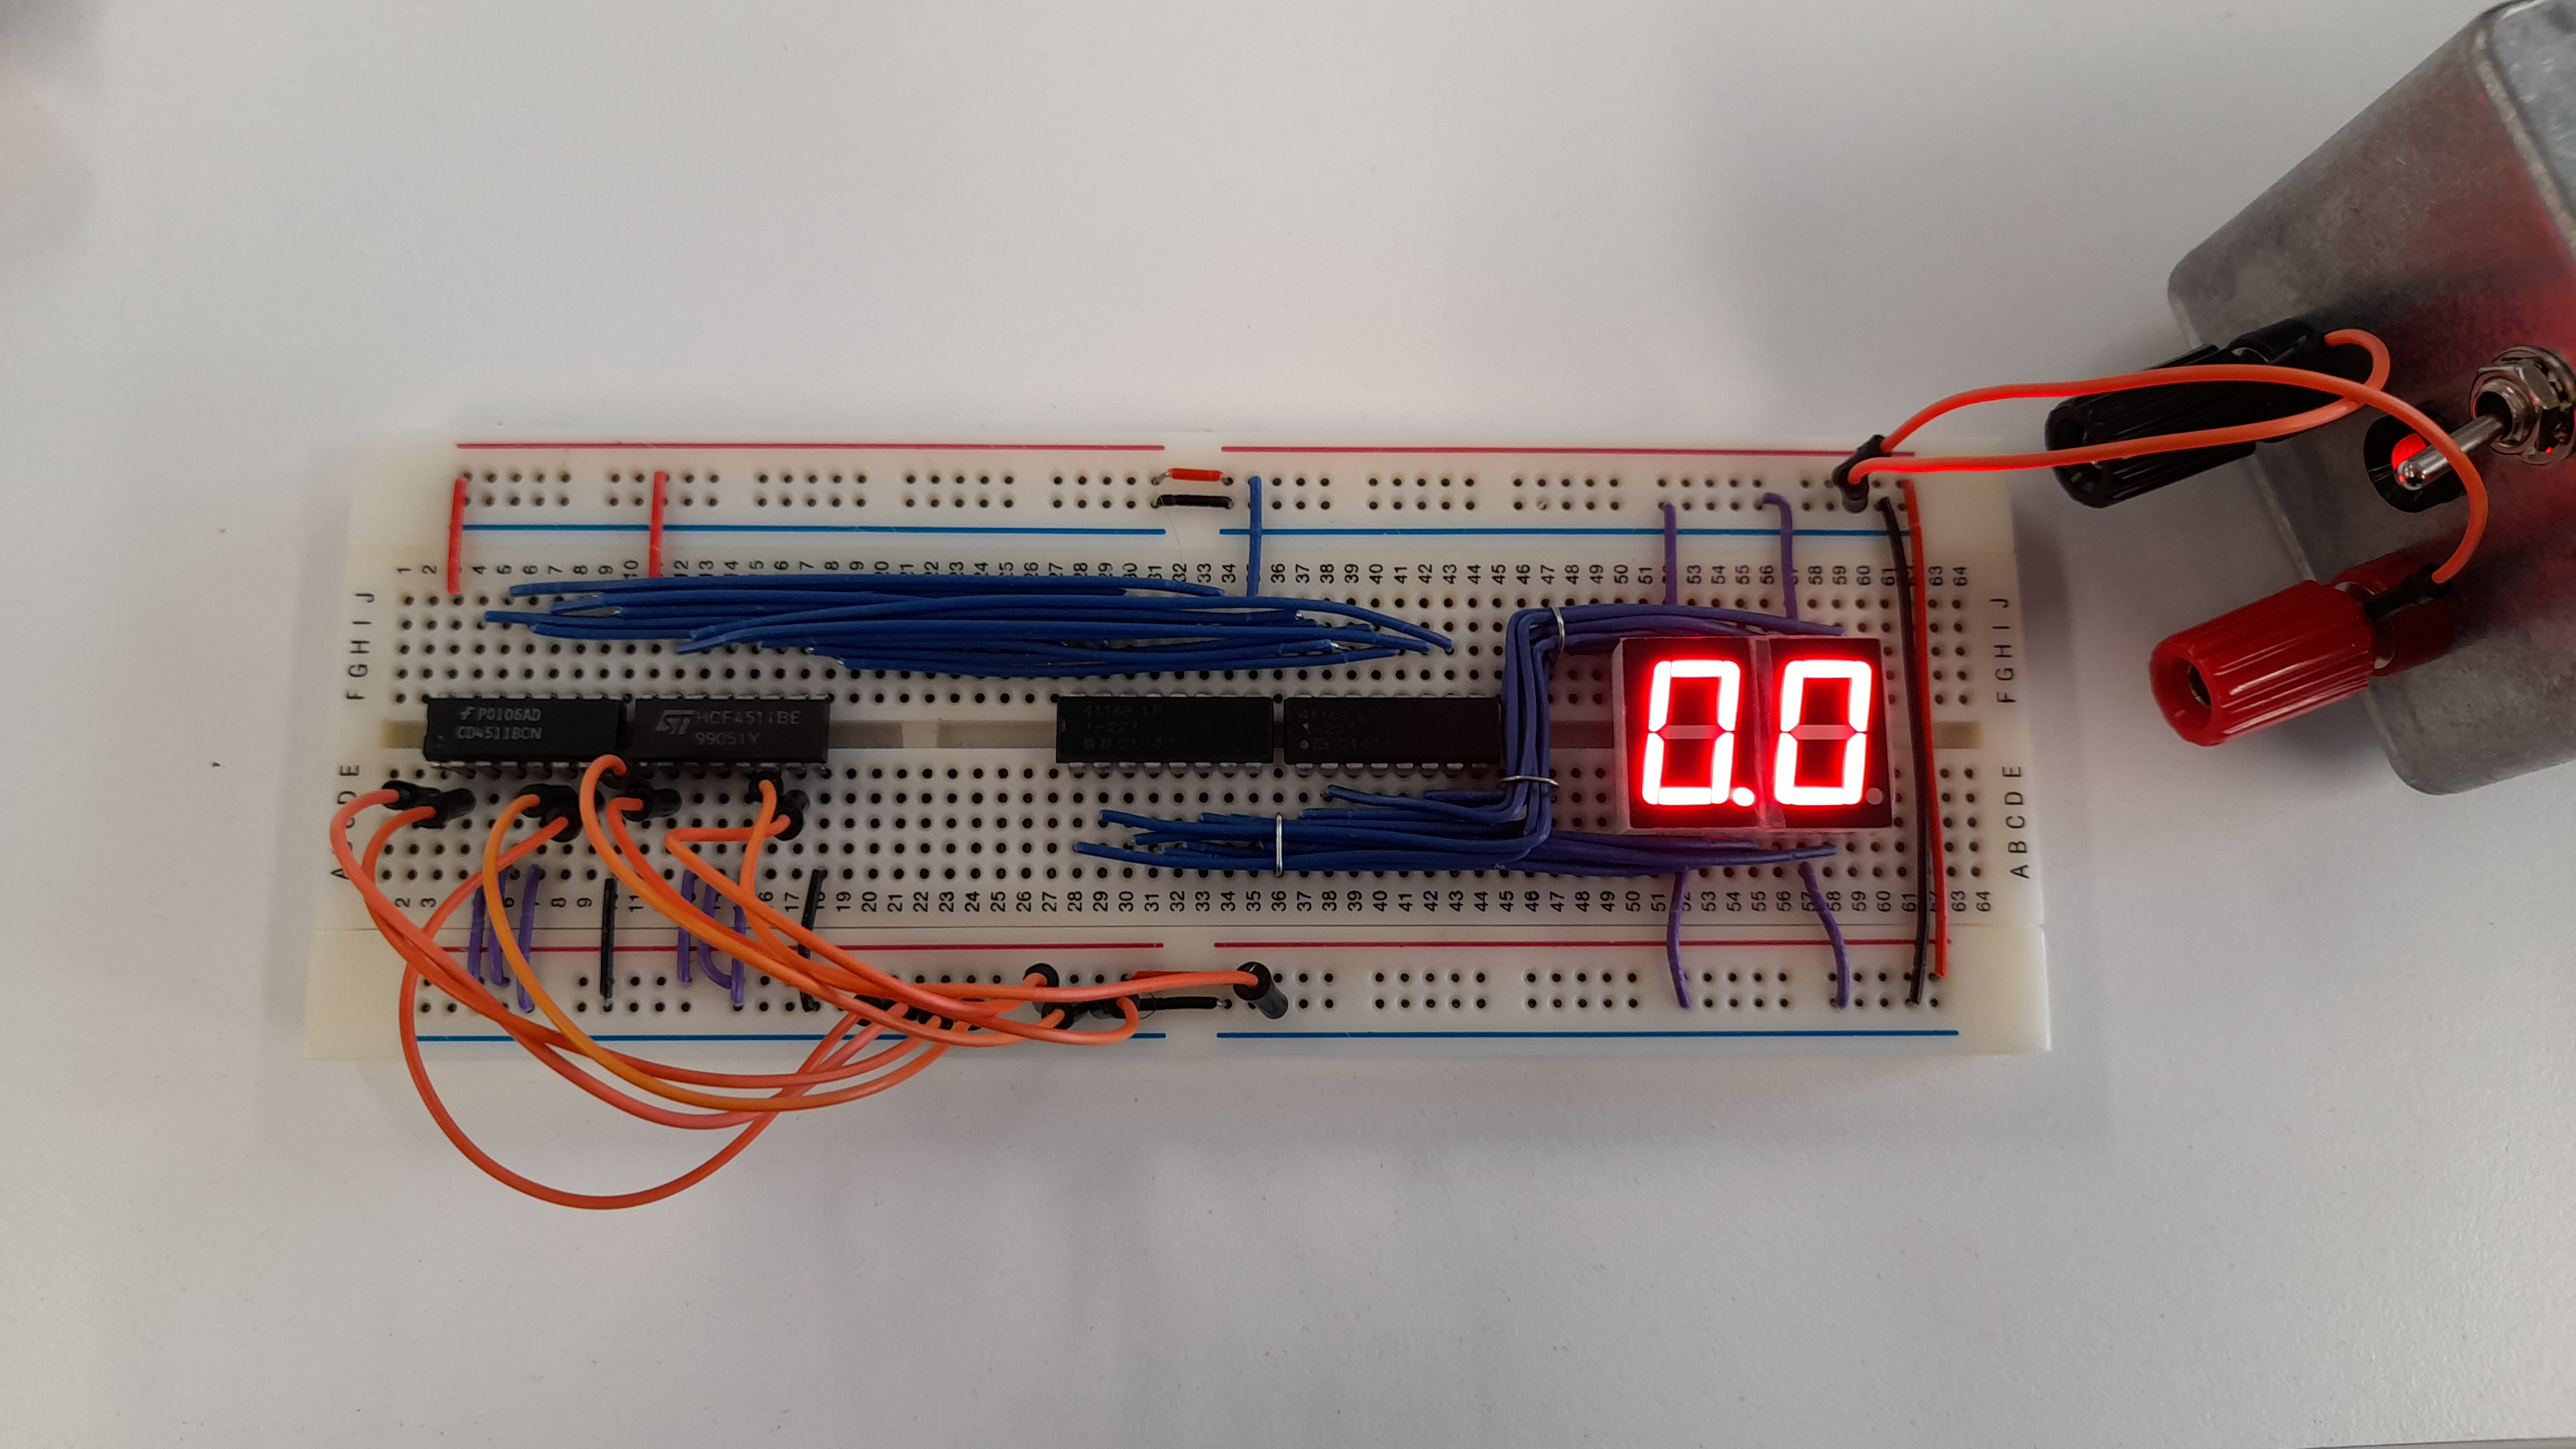
\includegraphics[width=0.9\textwidth]{images/displayTesting4.jpg}
        \caption{Neatened subsystem showing 0.0}
        \label{fig:displayTesting4}
    \end{minipage}
\end{figure}



\section{Memory Lookup Table Subsystem}
The memory subsystem is based off of an Electronically Erasable Programmable Read-Only Memory (EEPROM) chip.
The memory will work by using the value which has been latched onto the latches from the ADC subsystem when the ADC has converted the analogue value from the input voltage.
The purpose of the EEPROM is to take a input value and convert it to the corresponding BCD value which has been programmed into it. 
This will then be fed into the display subsystem which will display the values.
\subsubsection{Design}
To begin designing this, I worked out the values which the EEPROM would take and what it would output. I used a Google Sheets spreadsheet to do this. This was then inputted into the programming software which will burn the data onto the chip. 
To calculate the values I used the following steps.
\begin{enumerate}
    \item List all values from 0 to 255 inclusive
    \item Calculate what exact voltage this value would correspond to using the equation \\$\displaystyle Voltage=\left(\frac{5}{256}\right)\times Value$
    \item Multiply this new value by 10, then round to zero decimal places.
\end{enumerate}
\begin{figure} [H]
    \centering
    \begin{minipage}[t]{0.45\textwidth}
        \centering
        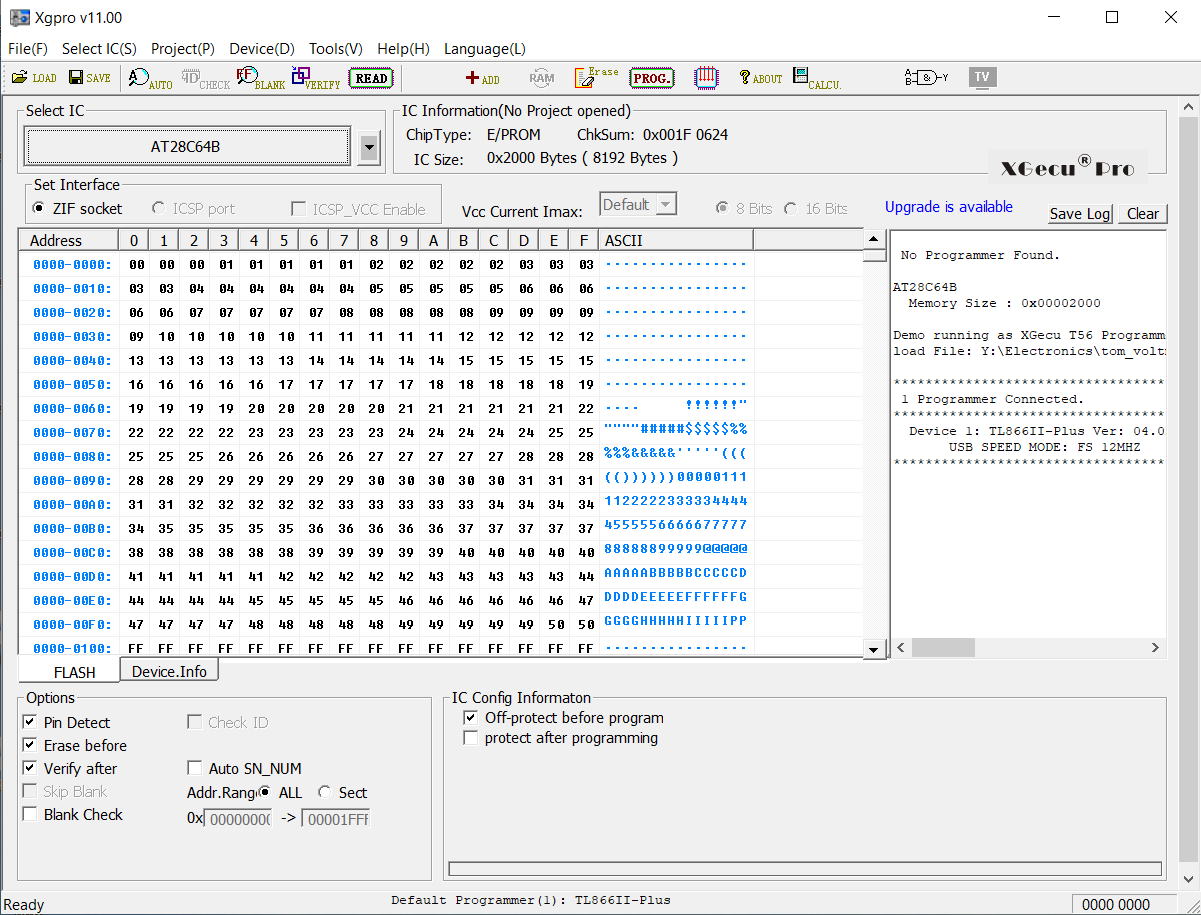
\includegraphics[width=0.9\textwidth]{images/eepromBurning1.png}
        \caption{The data ready to be burnt to the chip}
        \label{fig:eepromBurning1}
    \end{minipage}\hfill
    \begin{minipage}[t] {0.45\textwidth}
        \centering
        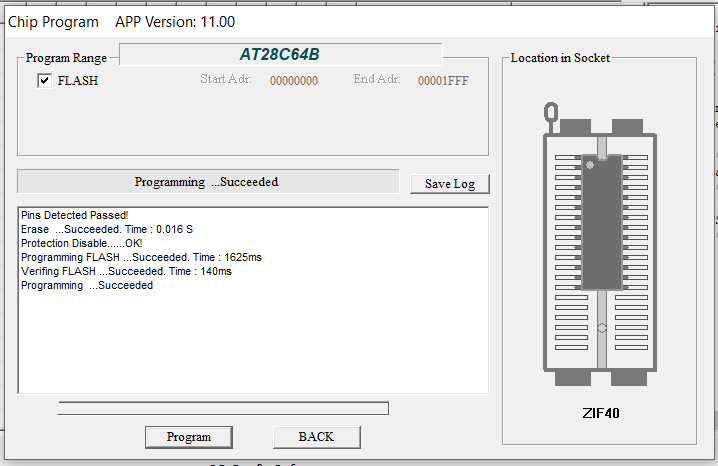
\includegraphics[width=0.9\textwidth]{images/eepromBurning2.png}
        \caption{The log output from the burning software}
         \label{fig:eepromBurning2}
    \end{minipage}
\end{figure}
\noindent I then worked out the schematic of the EEPROM.
\begin{figure}[H]
    \centering
    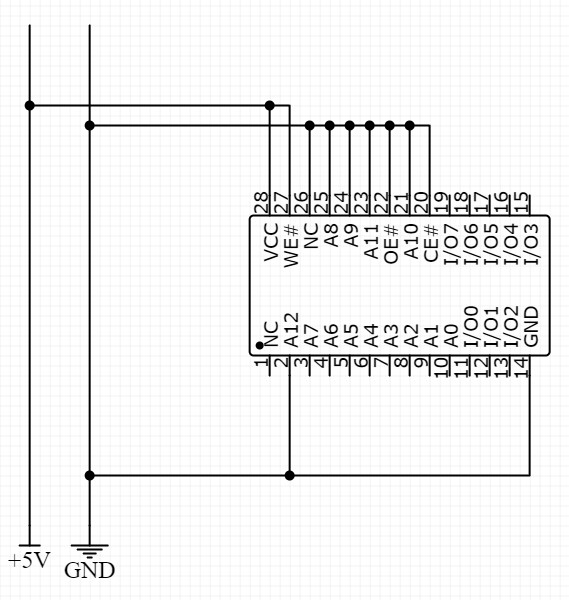
\includegraphics[width=0.5\textwidth]{images/eepromCircuitDiagram.jpg}
    \caption{Circuit diagram of the memory lookup table subsystem}
    \label{fig:eepromCircuitDiagram}
\end{figure}
\noindent Pins 3 through 10 inclusive will be connected to the output of the latches and pins 12, 13, 14 and 15 through 19 inclusive will be connected to the inputs of the display subsystem. These have been omitted from the diagram above for clarity and can be seen in the full schematic.\\
On the EEPROM chip, there are a number of pins which have to be tied either high or low, to allow it to output and to prevent overwriting the data which has been burnt to the chip. Pin 27 is write enable, this is active low so has to be tied high as we don't want to accidentally overwrite the data on the EEPROM. Pin 22 is output enable (again, active low), this has to be tied low as we want to output the data on the EEPROM. Pin 20 is chip enable (again, active low), this has to be tied low as we want to enable the chip to work.
\subsubsection{Building \& Testing}
To begin building this, I connected the outputs to inputs of the display subsystem, this would allow me to test if the EEPROM has been programmed correctly. I then connected the functional and power pins. Finally, I connected the inputs which I won't be using (as the EEPROM chip has a 14-bit input and I only need an 8-bit input) to 0V to ensure that they won't affect the address which the EEPROM is drawing data from. The inputs which I will be using, I initially connected to 0V (00000000). Now I am able to use jumper wires to imitate the binary sequence from the latches to ensure that the data has correctly been stored on the EEPROM and it is outputting as expected.
\begin{figure} [H]
    \centering
    \begin{minipage}[t]{0.45\textwidth}
        \centering
        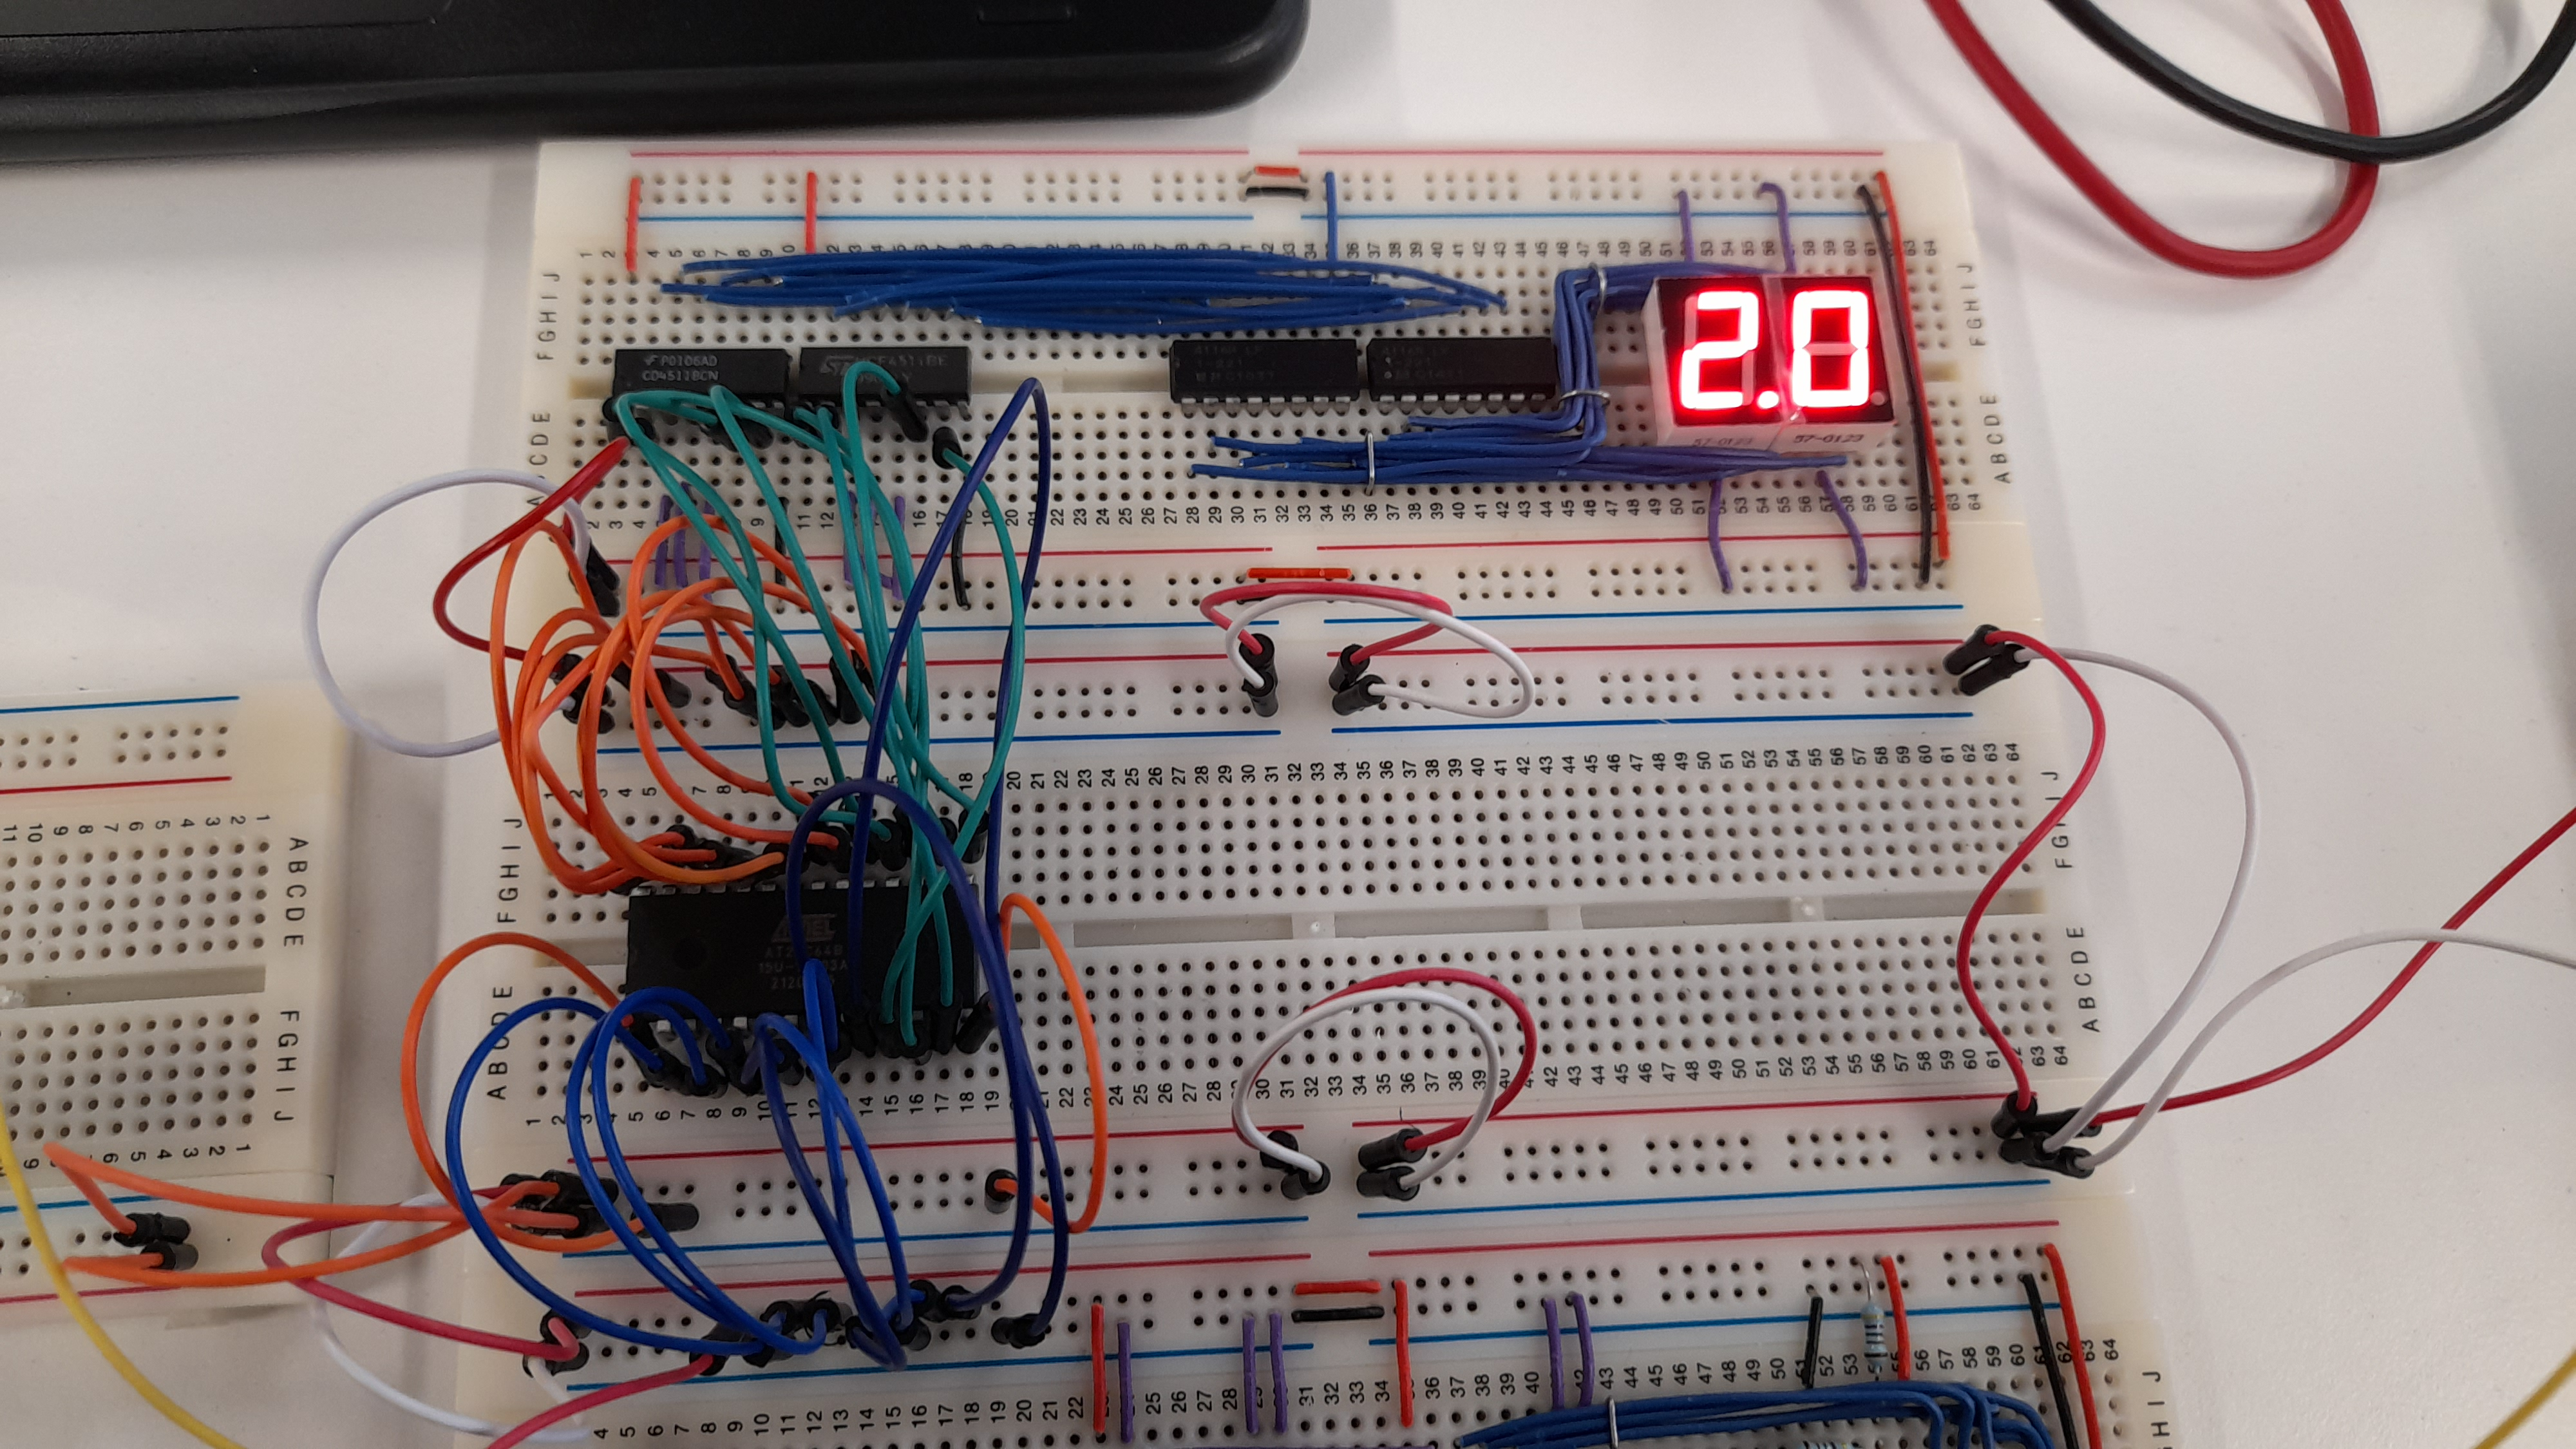
\includegraphics[width=0.9\textwidth]{images/eepromTesting1.jpg}
        \caption{Input: 01100110 and Output: 2.0}
        \label{fig:eepromTesting1}
    \end{minipage}\hfill
    \begin{minipage}[t] {0.45\textwidth}
        \centering
        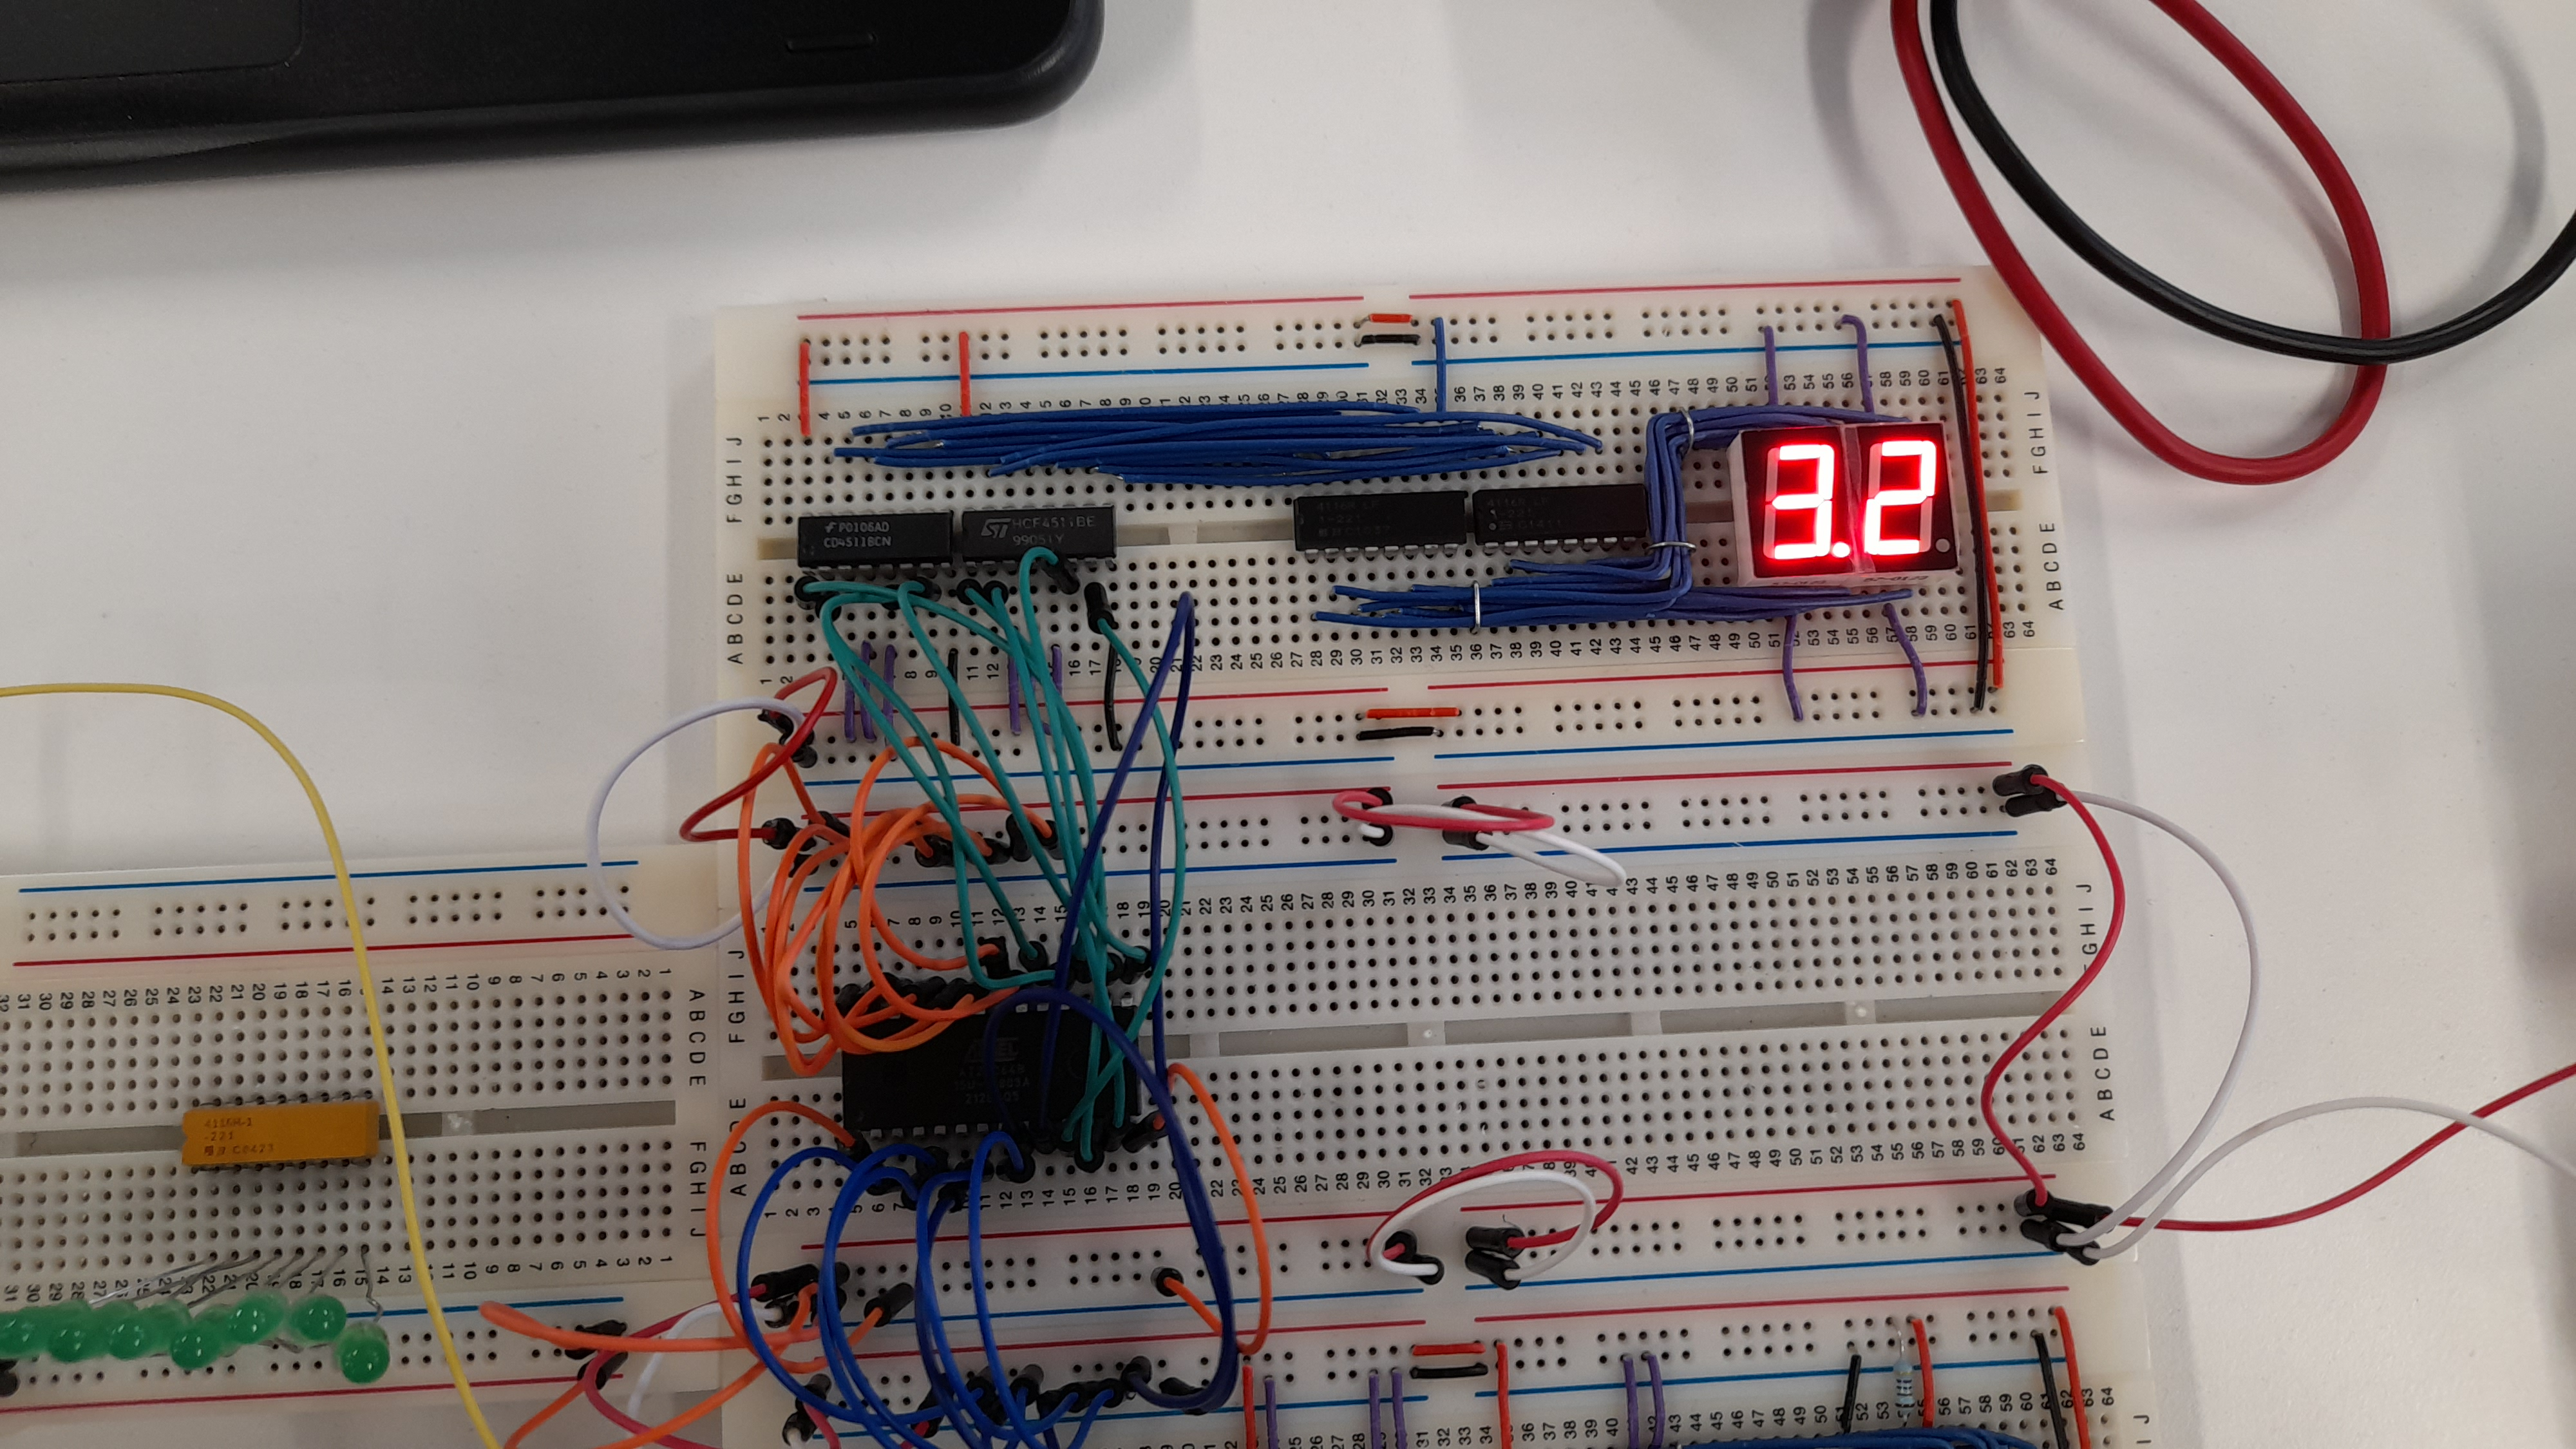
\includegraphics[width=0.9\textwidth]{images/eepromTesting2.jpg}
        \caption{Input: 10100010 and Output: 3.2}
         \label{fig:eepromTesting2}
    \end{minipage}
\end{figure}
\begin{figure} [H]
    \centering
    \begin{minipage}[t]{0.45\textwidth}
        \centering
        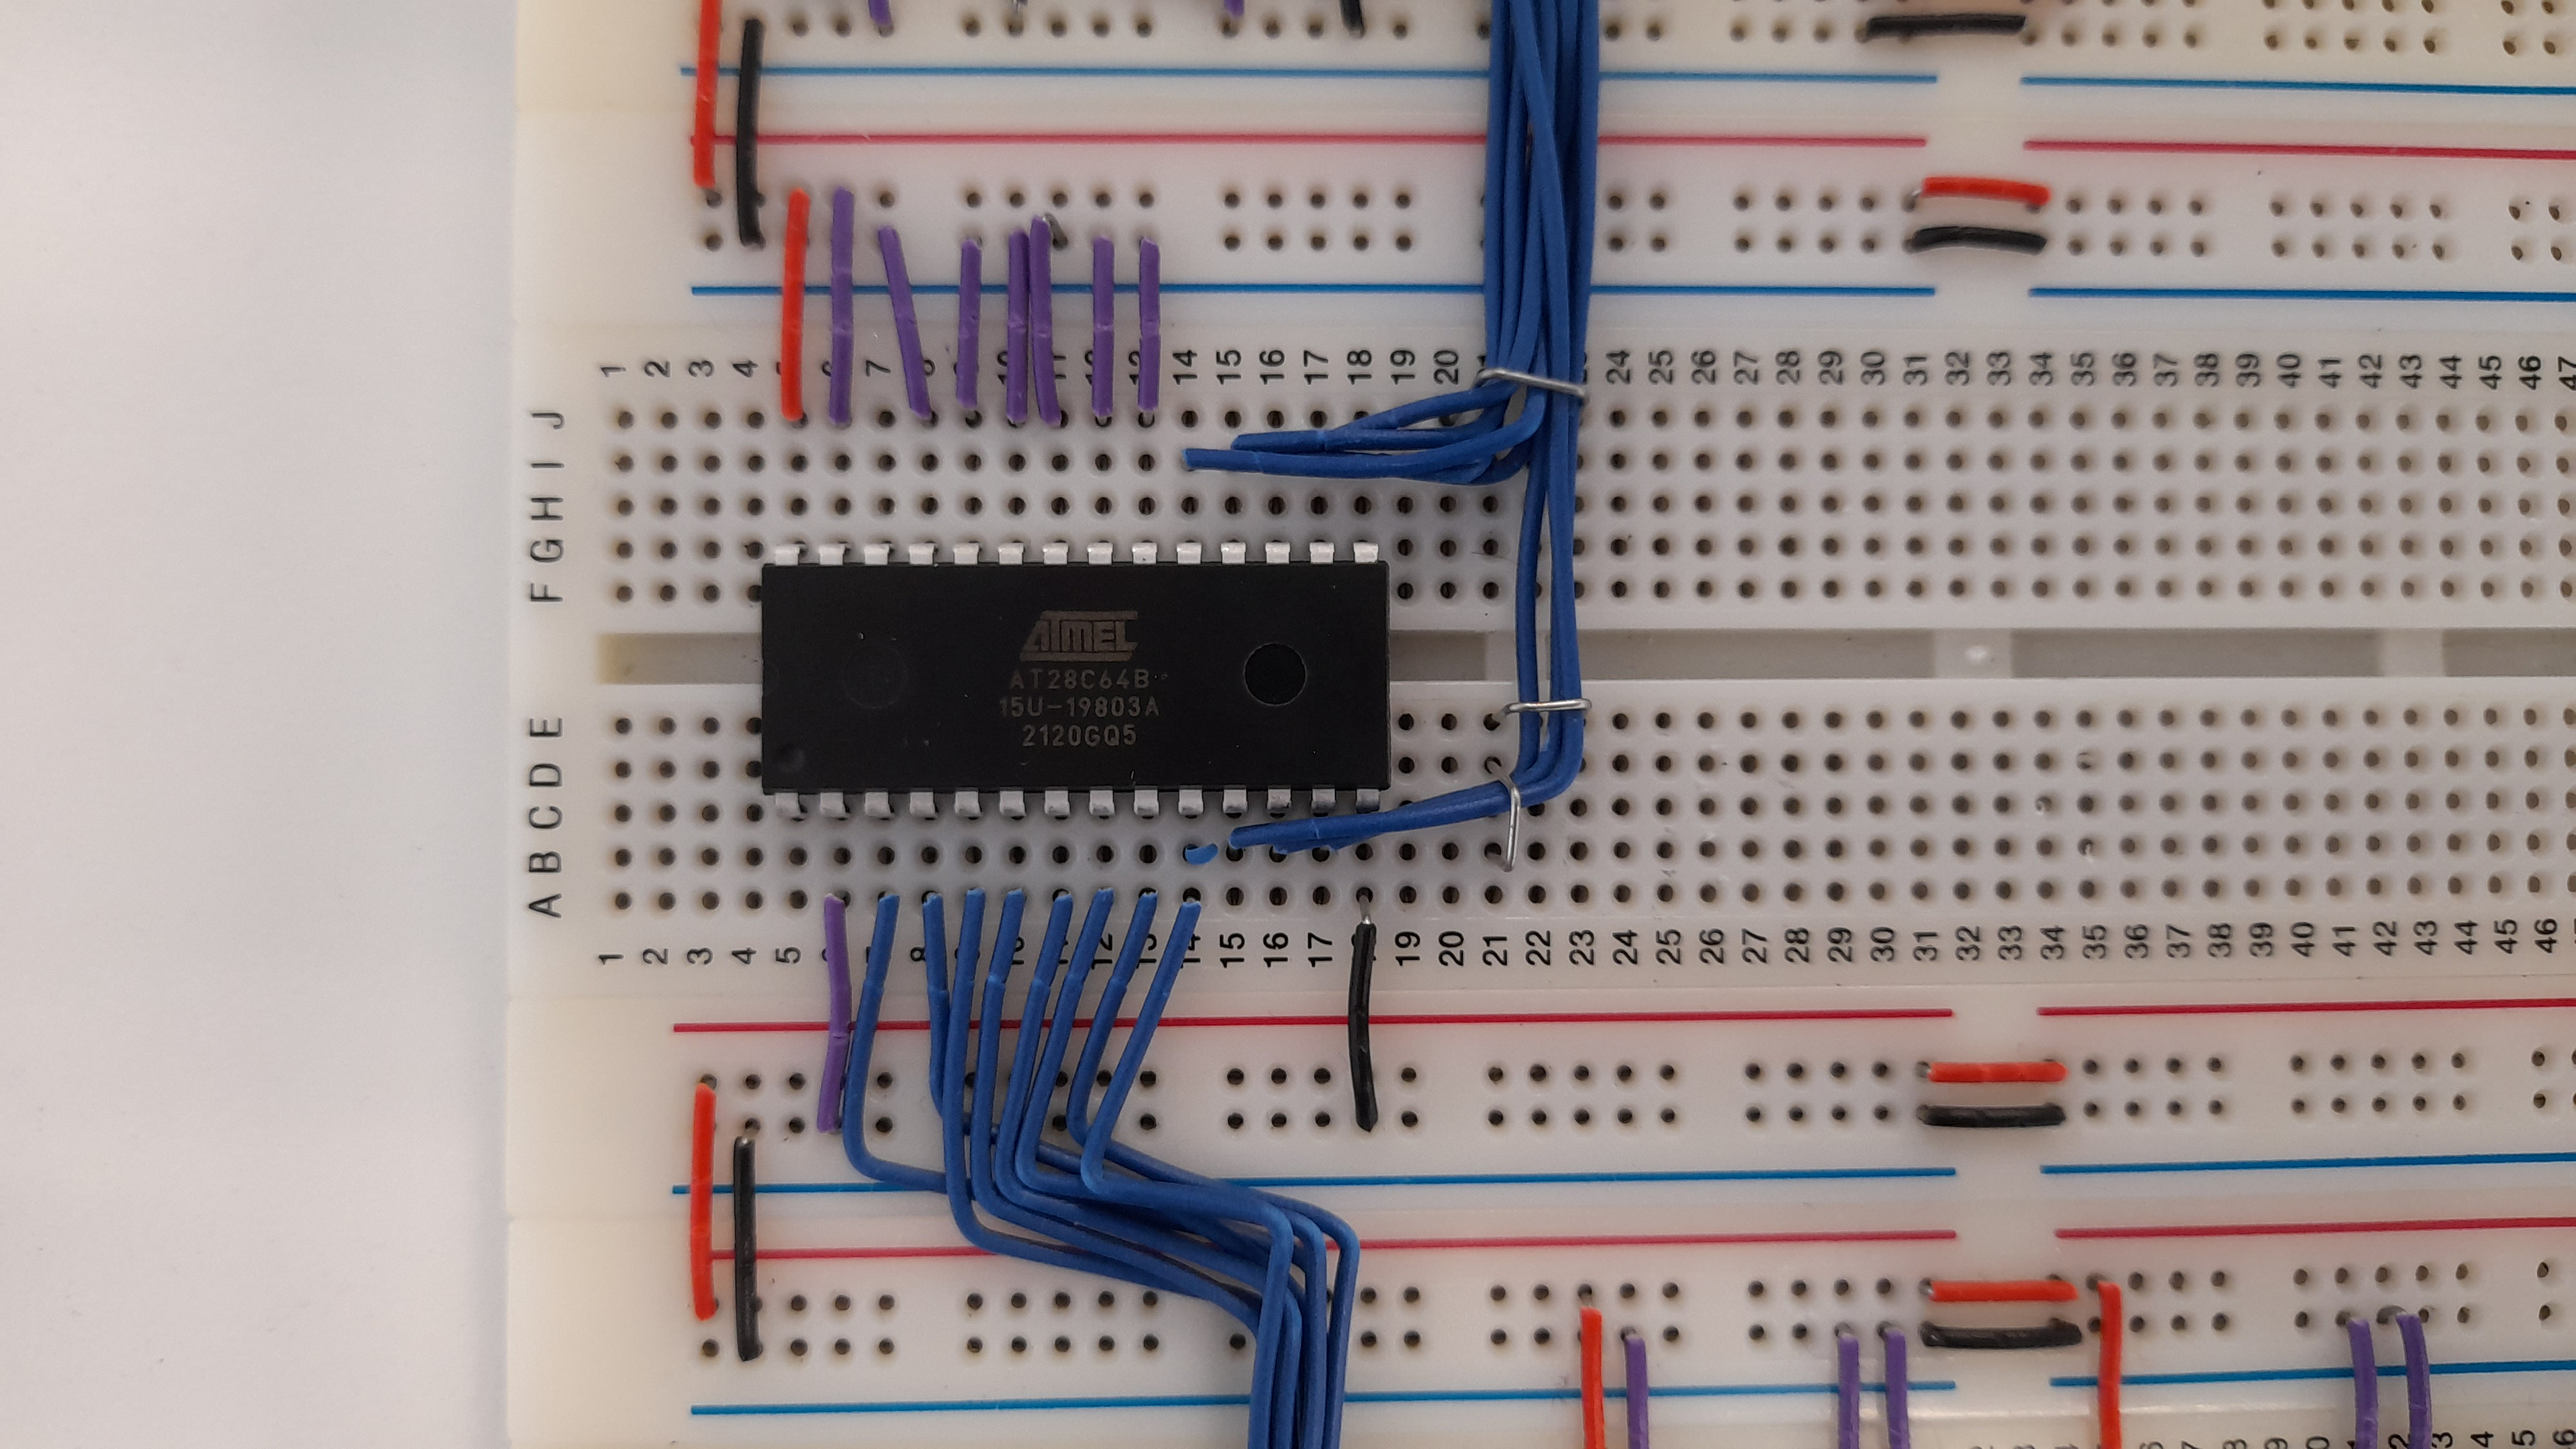
\includegraphics[width=0.9\textwidth]{images/eepromNeatened.jpg}
        \caption{Neatened EEPROM subsystem}
        \label{fig:eepromNeatened}
    \end{minipage}\hfill
    \begin{minipage}[t] {0.45\textwidth}
        \centering
    \end{minipage}
\end{figure}
\noindent Now I know that the data has correctly been stored on my EEPROM, I am able to connect the input to the EEPROM to the latch outputs; using a potentiometer for input to the circuit. Initially when I did this, the output wasn't displaying what I was expecting it to.  At this point, I was running out of time with the project, so I decided that due to the fact that the EEPROM was working on its own, I would be able to just neaten up the wires then test and troubleshoot the whole system together.\newline
An alternative subsystem I could have used instead of the EEPROM is a microprocessor. This would have been overkill for this project. \newline
\noindent I can now test the full system together. This can be found in chapter \ref{ch:testing}.